\documentclass[openleft]{kentigern}

\usepackage{lipsum}
\usepackage[acronym,toc]{glossaries}
\usepackage{siunitx}

\makeglossaries
\usepackage{tabularx}
\usepackage{type1cm}
\usepackage{lettrine}
\usepackage{physicsplus}
\usepackage{caption}

\usepackage{rotating}
\usepackage{pgfgantt}

\usepackage{setspace}
    \linespread{1.25}

\title{Year 2 Report}
\author{Daniel Williams}

%% This file is intended to contain all of the macros defining the
%% various mathematical and physical quantities used in this document in
%% order to maintain notational consistency throughout the document and
%% its glossary.

% Margin notes

\newcommand{\marginnote}[1]{
        \refstepcounter{footnote}
\footnotemark\marginpar{\footnotemark}\footnotetext{#1}}


\NewEnviron{sidefigure}[2]{
  \sidebar{
    \BODY
    \captionof{figure}{#1 \label{#2}}
  }
}

\providecommand{\msolar}{\mathrm{M{_\odot}}}
\providecommand{\mat}[1]{\mathsf{#1}}
\providecommand{\ex}{\mathbb{E}\,}

% New Operators
\DeclareMathOperator{\vary}{var}
\DeclareMathOperator{\cov}{cov}
\providecommand{\rmse}{\mathrm{RMSE}}

% Calculus operators
\providecommand{\dd}{\,\mathrm{d}}

% Software Packages
\providecommand{\imrphenomp}{\texttt{IMRPhenomP}}
\providecommand{\lalsim}{\texttt{LALSimulation}}

% New Units
\providecommand{\solMass}{\ensuremath{\mathrm{M}_{\odot}}}
%\DeclareSIUnit\parsec{pc}

% Galactic astronomy
\providecommand{\numberGalaxies}{N_\mathrm{G}}

% Gravitational wave detectors
\providecommand{\horizonDistance}{\ensuremath\mathcal{D}_{\mathrm{hor}}}

\providecommand{\GP}{\gls{gp}}

% Pipelines
\providecommand{\olib}{\texttt{oLIB}}
\providecommand{\cwb}{\texttt{cWB}}
\providecommand{\bayeswave}{\texttt{Bayeswave}}
\providecommand{\minke}{\texttt{Minke}}

% Software
\providecommand{\lalsuite}{\texttt{LALSuite}}
\providecommand{\lalsimulation}{\texttt{LALSimulation}}
\providecommand{\imrp}{\texttt{IMRPhenom\,v2}}
\providecommand{\seobnr}{\texttt{SEOBNR}}
\providecommand{\heron}{\texttt{heron}}
% latin
\providecommand{\map}{maximum \emph{a posteriori}}

% Gaussian processes
\providecommand{\set}[1]{\mathcal{#1}}
\providecommand{\gp}{\mathcal{G\!P}}
\providecommand{\GP}{Gaussian Process\renewcommand{\GP}{GP}}
\providecommand{\NR}{Numerical Relativity\renewcommand{\NR}{NR}}
\providecommand{\PE}{parameter estimation\renewcommand{\PE}{PE}}
\providecommand{\GW}{gravitational wave\renewcommand{\GW}{GW}}
\providecommand{\EI}{\mathbb{E} \mathrm{I}}

\providecommand{\trainingpoints}{\mathcal{X}}
\providecommand{\trainingobservations}{\mathcal{Y}}
\providecommand{\trainingdata}{(\trainingpoints, \trainingobservations)}

\providecommand{\kernel}[1]{\mathsf{#1}}
\providecommand{\SE}{\kernel{SE}}
\providecommand{\Con}{\kernel{C}}
\providecommand{\Lin}{\kernel{Lin}}
\providecommand{\Per}{\kernel{Per}}
\providecommand{\RQ}{\kernel{RQ}}
\providecommand{\Mat}{\kernel{M52}}

\providecommand{\numbertrainingpoints}{$12,325$}
\providecommand{\numbertrainingwaveforms}{no. Waveforms}



\theoremstyle{definition}
\newtheorem{definition}{Definition}[section]

\loadglsentries[main]{glossary/glossary.tex}


\usetikzlibrary{bayesnet}

\begin{document}
%\maketitle

\begin{titlepage}
\newgeometry{margin=2in}
\thispagestyle{empty}

\maketitle
\restoregeometry
\end{titlepage}

\newpage
%

%\tableofcontents
\newpage
%\vfill
\lettrine{I}{'ve had} the pleasure of being a member of the Institute for
Gravitational Research at the University of Glasgow for a little over
seven months. It would be difficult to deny that this has been an
unexpectedly eventful period in the life of the group, and it's been
great fun to experience the excitement of the first detection of a
gravitational wave as an insider (although an insider only by the skin
of my teeth), and to see the department's work on the LISA Pathfinder
mission come to fruition just a few months later.  

The work outlined in this report comprises a number of projects which
I have spent these seven months working on, however the first
observing run of Advanced LIGO proved more disruptive to my schedule
than was, perhaps, initially envisaged.
\vfill
\newpage

%%% Local Variables: 
%%% mode: latex
%%% TeX-master: "../document"
%%% End: 

% \part{Outline \& Review of Gravitational Wave Literature}
% \label{part:introduction}


\part{Introduction}
\label{part:intro}


 \chapter{Gravitational Waves}
 \label{cha:grav-waves}

%\section{Gravitational waves}
%\label{sec:gravwaves}
\chapterprecis{\Glspl{gravitational wave} were perhaps the last of the
  predictions of Einstein's General Theory of Relativity to be
  observed; their detection was the catalyst for the beginning of a
  new era of astrophysics}

\epigraph{I guess we need to do the detection checklist...}{\textbf{Sergey Klimencko}, \emph{Internal LSC communication}, 14 September 2015}

\lettrine[lines=3]{T}{he 14 September 2016} will likely be remembered as one of the most
significant in the history of astronomy and of astrophysics. Early in
the morning of this autumn day, shortly after 9am UT, a gravitational
wave passed through the Earth, and on its way produced a sufficiently
large movement in the mirrors and test masses of the detectors of the
Laser Interferometer Gravitational-wave Observatory (\gls{LIGO}), as to be
detected.

Over five months of data analysis, detector characterisation, and
detection verification were conducted by a global team of scientists,
in the LIGO and VIRGO Scientific Collaboration (LVC). This process
resulted in a slew of journal papers being written, vast quantities of
data produced, and an enormous public outreach effort to be
launched. Eventually, the collaboration found itself in a position to
make the announcement of the first direct detection of gravitational
waves, GW150914, on 11 February 2016.

GW150914 is not the first evidence for gravitational waves, with the
Hulse-Taylor pulsar\cite{1975ApJ...195L..51H,2005ASPC..328...25W}
having provided compelling indirect evidence which lead to its
discoverers receiving the 1993 Nobel Prize.

%%% Local Variables: 
%%% mode: latex
%%% TeX-master: "../../document"
%%% End: 



% \section{Gravitational waves and general relativity}
% \label{sec:grav-waves-gener}
% Gravitational waves are one of the predictions of Einstein's 1915
Theory of General Relativity.


The Einstein field equations are non-linear, and analytical solutions
aren't possible. In order to perform calculations in general
relativity it is possible to turn to  \emph{post-Newtonian} expansion. 

The lowest-order expansion from which radiation is produced is the
quadrupole order, which depends upon the density and velocity field of
the system. The quadrupole tensor is defined
\begin{equation}
  \label{eq:1}
  Q_{jk} = \int \rho x_k x_k \dd[3]{x}
\end{equation}
and the gravitational wave is described by the three-tensor
\begin{equation}
  \label{eq:2}
  h_{jk} = \frac{2}{r} \dv[2]{Q_{jk}}{t}
\end{equation}


%%% Local Variables: 
%%% mode: latex
%%% TeX-master: "../../document"
%%% End: 


\section{GW150914: The first detection}
\label{sec:gw150914:-first-dete}
The first detection of gravitational waves was announced by the LIGO
Scientific Collaboration and the VIRGO Collaboration on 11 February
2016\cite{2016PhRvL.116f1102A}.


%%% Local Variables: 
%%% mode: latex
%%% TeX-master: "../../document"
%%% End: 



 \chapter{Detectors}
 \label{cha:detectors}

 \chapterprecis{Gravitational wave detectors are one of the great
   achievements of Twentieth and early Twenty-First Century
   science. They are the most sensitive measuring devices ever
   constructed, but they face numerous technical challenges.}

%\section{Gravitational wave detectors}
%\label{sec:detectors}

The earliest attempts to develop a gravitational wave detector were
made in the 1960s with the experiments of Jospeh Weber (1919--2000) at
the University of Maryland, from which he claimed the first detection
in 1969\cite{1969PhRvL..22.1320W,1970PhRvL..24..276W} of signals
originating in the galactic centre\cite{1970PhRvL..25..180W}. Numerous
attempts to confirm his findings were unsuccessful, including searches
in Drever's group at the University of Glasgow
\cite{1973Natur.246..340D} in the UK, at Bell Labs
\cite{1973PhRvL..31..173L,1973PhRvL..31..176G,1974PhRvL..33..794L} in
the USA, at Munich\cite{1975NCimL..12..111B,1975NCimL..12..111B} in
Germany, at Moscow\cite{1973PhLA...45..271B} in Russia, and at
Tokyo\cite{1975PhRvL..35..890H} in Japan. While Weber's original
detections were soundly refuted by the community there is little doubt
that the announcement led to a flurry of activity in the field. This
lead to the development of modern cryogenic resonant bars, such as
ALTAIR\cite{1992NCimC..15..943B}, ALLEGRO\cite{2000IJMPD...9..229M},
NAUTILUS\cite{1997APh.....7..231A}, and
EXPLORER\cite{1993PhRvD..47..362A}; and laser interferometers.

Laser interferometers, of which advanced LIGO is an implementation,
were the result of a quest for both higher sensitivities and
bandwidth. The possibility of using a Michelson interferometer to
measure the distance between test masses in order to detect
gravitational radiation originated in Moscow\cite{1963JETP...16..433G}
in 1963.  This approach was followed early-on by Scottish and German
groups as a means of improving on resonant bar sensitivities, with a
3-meter and later a 30-meter prototype detector constructed at
Garching in the late
1970s\cite{1979JPhE...12.1043B,1988PhRvD..38..423S} which used optical
delay lines, and a 1-meter prototype, and later a 10-meter instrument
were built at Glasgow in the early
1980s\cite{1979RSPSA.368...11D,1995RScI...66.4447R}, which used
Fabry-Perot cavities . The Glasgow detector was the spiritual
predecessor to the CalTech 40-meter
prototype\cite{1996PhLA..218..157A}. The increasing maturity of
technology developed by these prototypes lead to the construction of
the first generation of long-baseline detectors, starting with TAMA in
Tokyo\cite{1996JKASS..29..279K}, the joint UK-German GEO600
detector\cite{1997CQGra..14.1471L} near Hannover, and the two
kilometre-scale detectors, the joint CalTech-MIT detectors
LIGO\cite{1992Sci...256..325A}, located at two sites in the USA, and
the joint Italian-French detector VIRGO\cite{1990NIMPA.289..518B},
near Cascina. These detectors were operated during the 2000s, and
while none of them made a detection of gravitational waves, they
provided valuable astrophysical results by placing astrophysical
limits on the strength of the stochastic gravitational wave background
\cite{2014PhRvL.113w1101A}, production of gravitational waves by
pulsars\cite{2014ApJ...785..119A} and gamma ray
bursts\cite{2012ApJ...760...12A}, and the rate of compact binary
coalescence in the local
universe\cite{2012PhRvD..85h2002A,2013PhRvD..87b2002A}.

The initial-generation of detectors were upgraded during the first
half of the 2010s, leading to Advanced LIGO\cite{2015CQGra..32g4001L}
which resumed observations in September 2015, and the imminent start
of observations from the Advanced VIRGO
detector\cite{2015CQGra..32b4001A}, with the prospect of a joint run
occuring during the second half of 2016. The GEO detector was the
first of the initial detectors to be fully upgraded becoming GEO-HF
\cite{2006CQGra..23S.207W}, with improved sensitivity at high
frequencies. Japanese efforts have focussed on the development of
KAGRA (formerly LCGT), a cryogenic interferometer located deep
underground in the Kamioka mine\cite{1999IJMPD...8..557K}, although
the project has suffered from a number of set-backs. The construction
of a third LIGO detector interferometer in India using the mothballed
second detector from the Washington site has now moved into its
initial stages, with the prospect of this detector joining the network
around the end of the decade.

The second-generation detectors, specifically the two Advanced LIGO
detectors were responsible for the first discovery of gravitational
waves\cite{2016PhRvL.116m1103A}, and have successfully demonstrated
the ability of interferometry to observe the gravitational
universe. This said, future improvements in sensitivity are highly
desirable, but are likely to be even more technically challenging than
the transition from resonant bars to laser interferometers. In order
to improve the bandwidth of detectors a location free of
\emph{Newtonian noise} must be found, which ultimately mandates the
placement of an interferometer in space. There have been a number of
proposals for a space-based interferometer, with
eLISA\cite{2013GWN.....6....4A} likely to be the first to launch in
the 2020s, following the completion of a pathfinder mission during
2016\cite{2015JPhCS.610a2005A}. NEED TO UPDATE THIS. The eLISA detector will be sensitive
in the milli-hertz region of the gravitational wave spectrum, and will
be capable of observing binary inspirals at a much earlier stage in
their evolution than the advanced ground-based detectors, as well as
the galactic population of low-mass binaries, such as binary white
dwarfs. A Japanese proposal, DECIGO\cite{2011CQGra..28i4011K}, would
observe in the decihertz regime using a complex arrangement of six
spacecraft in a star-of-David confugration. There are also plans for
more sensitive detectors on the ground. The Einstein telescope is a
European proposal for an underground kilometre-scale detector in a
triangular configuration, using a ``xylophone'' configuration to
improve broadband sensitivity compared to the second-generation of
detectors; its scientific aims include providing more sensitive tests
of general relativity than are possible with the advanced
detectors\cite{2012CQGra..29l4013S}. There are also proposals for
upgrades of the advanced detectors to use squeezed light to reduce
quantum noise\cite{2015PhRvD..91f2005M}, the use of
speedmeters\cite{2014MUPB...69..519V,2002gr.qc....11088K}, or atom
interferometry\cite{2013PhRvL.110q1102G,2016PhRvD..93b1101C,2008PhRvD..78l2002D}.

At the very low-frequency limit of the gravitational wave spectrum the
bulk of detection efforts rotate around pulsar timing arrays, which
promise the detection of gravitational waves by precision measurements
of pulse arrival times from a number of pulsars distributed across the
sky. By observing correlated delays\cite{1983ApJ...265L..39H} in
arrival times the presence of a very long wavelength gravitational
wave can be inferred. There are a number of collaborations actively
producing pulsar observations with the aim of detecting gravitational
waves: the European Pulsar Timing Array
(EPTA)\cite{2013CQGra..30v4009K}, NANOGrav\cite{2009arXiv0909.1058J},
the Parkes Pulsar Timing Array (PPTA)\cite{2013PASA...30...17M}, and
the International Pulsar Timing Array (IPTA)
collaboration\cite{2013CQGra..30v4010M}.

%%% Local Variables: 
%%% mode: latex
%%% TeX-master: "../../document"
%%% End: 


% \section{Detector architectures}
% \label{sec:detect-arch}

% \section{Resonant bar detectors}
% \label{sec:reson-bar-detect}

 % \section{Ground-based interferometers}
 % \label{sec:ground-based-interf}
 % The cutting-edge of current ground-based interferometers are the twin
Advanced LIGO detectors \cite{2015CQGra..32g4001L} located in Hanford,
WA, USA, and Livingston, LA, USA. These interferometers are Michelson
interferometers with a large number of additional components, which
allow detection of differential changes in their arm lengths (strains)
on the order of $10^{-22}$.

% \begin{figure}
% \begin{adjustwidth*}{-5.5in}{-2in}
%   \centering
%   %\begin{tikzpicture}[
	scale=0.8,
	housing/.style={top color=black!10, bottom color=black!40, draw=black!50, line width=1pt},
]

\begin{scope}[]
%%% CORNER STATION

\draw [housing] (0,0) rectangle (5,5) node at (1.5,-.4) {Corner Station};

\draw [housing] (1.5,5) rectangle (3.5,15);
\draw [housing] (1.5,17) rectangle (3.5,19);
\end{scope}

\begin{scope}[]
%%% X ARM
\draw [housing] (5,1.5) rectangle (15,3.5);
\draw [housing] (17,1.5) rectangle (19,3.5);
\end{scope}

\end{tikzpicture}
%   \caption{An interferometer.}
%   \label{fig:interferometer}
% \end{adjustwidth*}
% \end{figure}

\subsection{Detecting gravitational waves with light}
\label{sec:interferometricdetection}

Gravitational-wave detectors which use beams of light, such as
interferometers and pulsar timing arrays rely on measuring the the
travel time of a beam of electromagnetic radiation between two points,
and the effect that a gravitational wave has on this time. A full
treatment of this is given in \cite{2009LRR....12....2S}, but in
summary, if a gravitational wave is not present within a detector, the
travel time of a beam will be constant. If a gravitational waev is
introduced, which has a polarisation component $h_+(t)$ in the plane
of the beam, the change in the arrival time of the beam will be
\begin{equation}
  \label{eq:arrival-times-gw}
  \dv{t_f}{t} = 1 + \half (1 + \cos(\theta)) \qty{ 
    h_+\qty( t + [1- \cos(\theta) ] L) - h_+(t) 
  }
\end{equation}
where $\theta$ is the angle separating the detector beam and the
gravitational wave plane, and $L$ is the proper distance separating
the clocks when no gravitational wave is present.

By arranging the detector to reflect the beam back to the originating
clock, it is possible to measure the round-triop time using only one
clock. In this arrangement we must account for the gravitational wave
having a different strength one the return trip, and so equation
(\ref{eq:arrival-times-gw}) becomes 
\begin{align}
  \label{eq:three-term}
  \dv{t~{round}}{t} = 1 + \half \Big(  (& 1-\cos(\theta) )h_+ (t+2L) - (1+\cos(\theta))h_+(t) \nonumber \\ & + 2 \cos(\theta) h_+ [t+L(1 - \cos(\theta))] \Big)
\end{align}
the \emph{three-term} relation.

\subsection{Operation of a Michelson interferometer}
\label{sec:Michelson}
%
\sidebar{
\begin{center}
  \begin{tikzpicture}
    \draw [thick, red] (0,0.25) -- (3,0.25);
    \draw [thick, red] (1.1, 0.25) -- (1.1, 2.15);
    \draw [thick, red, dashed] (1.1, 0.25) -- (1.1, -0.5);
    \fill (0,0) rectangle (0.5, 0.5);
    \draw [ultra thick] (0.95, 0.1) -- +(45:.4);
    \draw [ultra thick] (3, 0) rectangle (3.2, .5);
    \draw [ultra thick] (0.8, 2.15) rectangle (1.4, 2.35);
  \end{tikzpicture}
\end{center}
\captionof{figure}{A simple Michelson interferometer, composed of a
    light source (black box), a beam splitter (heavy black line), and
    two end mirrors (white boxes). \label{fig:michelson}}
} 
%
A Michelson interferometer is an optical device which is capable of
measuring the difference in length between two optical paths to
sub-wavelength precision. A Michelson interferometer can be
constructed using a beamsplitter and two mirrors, in the configuration
presented in figure \ref{fig:michelson}. The input beam is split along
the $x$ and $y$ directions, and reflected back to the
beam-splitter. At the beam-splitter the two beams will interfere: in
the standard Michelson setup this will result in constructive
interference if the arms have identical lengths, and a beam will be
produced at the output (the dashed red line). If the arms' relative
lengths change a pattern of interference fringes will be visible at
the output of the interferometer.

\subsection{Power Recycling}
\label{sec:power-recycling}
%
\sidebar{
\begin{center}
  \begin{tikzpicture}
    \draw [ultra thick, red] (0,0.25) -- (3,0.25);
    \draw [ultra thick, red] (1.1, 0.25) -- (1.1, 2.15);
    \draw [thick, red] (-1,0.25) -- (0, 0.25);
    \draw [thick, red, dashed] (1.1, 0.25) -- (1.1, -0.5);
    \fill (-1,0) rectangle (-0.5, 0.5);
    \draw [ultra thick] (0.95, 0.1) -- +(45:.4);
    \draw [ultra thick] (3, 0) rectangle (3.2, .5);
    \draw [ultra thick] (0.8, 2.15) rectangle (1.4, 2.35);
    \draw [ultra thick] (-0.25, 0) rectangle (-0, 0.5);
  \end{tikzpicture}
\end{center}
\captionof{figure}{A Michelson interferometer with power recycling,
  using a comparable setup to figure \ref{fig:michelson}, but with a
  mirror added between the laser and the beam splitter. \label{fig:power-recycle}}
} 
%
The optimal signal-to-noise ratio can be achieved from an
interferometer when the arm lengths are configured so that when no
gravitational wave is present in the interferometer the interferometer
beams interfere destructively \cite{1978JPhE...11..710E}. If the
mirrors are low loss the light will then be reflected back towards the
laser, and by placing a mirror between the laser and the beam splitter
a resonant cavity can be formed (see figure \ref{fig:power-recycle}),
allowing the power in the interferometer to build up. This allows a
less powerful laser to be used as the input for the interferometer,
with a \SI{10}{\watt} laser capable of providing several kilowatts of
power inside the interferometer \cite{2011LRR....14....5P}.

\subsection{Signal Recycling}
\label{sec:signal-recycling}
%
\sidebar{
\begin{center}
  \begin{tikzpicture}
    \draw [thick, red] (0,0.25) -- (3,0.25);
    \draw [thick, red] (1.1, 0.25) -- (1.1, 2.15);
    \draw [thick, red] (-1,0.25) -- (0, 0.25);
    \draw [thick, red, dashed] (1.1, 0.25) -- (1.1, -1.0);
    \fill (-1,0) rectangle (-0.5, 0.5);
    \draw [ultra thick] (0.95, 0.1) -- +(45:.4);
    \draw [ultra thick] (3, 0) rectangle (3.2, .5);
    \draw [ultra thick] (0.8, 2.15) rectangle (1.4, 2.35);
    \draw [ultra thick] (0.9, -0.5) rectangle (1.3, -0.7);
  \end{tikzpicture}
\end{center}
\captionof{figure}{A Michelson interferometer with signal recycling,
  using a comparable setup to figure \ref{fig:michelson}, but with a
  mirror added between the output and the beam splitter. \label{fig:signal-recycle}}
} 
%
Signal recycling can be used to tune the bandwidth of an
interferometer, and to increase its sensitivity by re-injecting the
interferometer's output signal to the interferometer, achieving
resonance, which increases the signal-to-noise ratio of the
signal. This is possible thanks to the sidebands on the beam which are
produced by the gravitational wave not interfering destructively.

To perform signal recycling a mirror is added between the
beam-splitter and the readout port of the interferometer, with this
configuration illustrated in figure \ref{fig:signal-recycle}.

\subsection{Fabry-Perot Cavities}
\label{sec:fabry-perot-cavities}
%
\sidebar{
\vspace{-1cm}
\begin{center}
  \begin{tikzpicture}
    \draw [thick, red] (0,0.25) -- (3,0.25);
    \draw [thick, red] (1.1, 0.25) -- (1.1, 2.15);
    \draw [thick, red] (-1,0.25) -- (0, 0.25);
    \draw [thick, red, dashed] (1.1, 0.25) -- (1.1, -1.0);
    \fill (-1,0) rectangle (-0.5, 0.5);
    \draw [ultra thick] (0.95, 0.1) -- +(45:.4);
    \draw [ultra thick] (3, 0) rectangle (3.2, .5);
    \draw [ultra thick] (0.8, 2.15) rectangle (1.4, 2.35);
    \draw [ultra thick] (0.9, -0.5) rectangle (1.3, -0.7);
  \end{tikzpicture}
\end{center}
\captionof{figure}{A Michelson interferometer with signal recycling,
  using a comparable setup to figure \ref{fig:signal-recycle}, but with a
  mirror added between the beam-splitter and the end mirrors of each arm. \label{fig:fabry-perot}}
}
%
The arms of modern interferometers used in the detection of
gravitational-waves store the beam for a period of time comparable to
the timescale of the signals which are being searched for. In the case
of kilometre-scale detectors and signals with a period around
\SI{1}{\milli\second} this implies the need for the light to reflect
up-and-down the detector around $50$ times. This is achieved by laying
the reflected beams atop each other in a Fabry-Perot cavity, with a
\gls{finesse}, $\mathcal{F}=50$. A Fabry-Perot cavity is formed by
placing a mirror between the beam-splitter and the end mirror in each
arm, as illustrated in figure \ref{fig:fabry-perot}.

\subsection{Advanced LIGO}
\label{sec:advanced-ligo}

The Advanced LIGO detectors are 4-kilometre long interferometers with
Fabry-Perot cavities, with a finesse of 50. The detectors improve
their sensitivity compared to the initial generation detectors through
the use of signal recycling, a technology pioneered in the GEO
detector, and have quadruple mirror suspensions which use fused silica
fibres to provide seismic
islolation\cite{2002CQGra..19.4043R,2012CQGra..29w5004A}.
  \begin{figure}
  \centering
  \scalebox{0.5}{
  \newcommand{\convexpath}[2]{
  [   
  create hullcoords/.code={
    \global\edef\namelist{#1}
    \foreach [count=\counter] \nodename in \namelist {
      \global\edef\numberofnodes{\counter}
      \coordinate (hullcoord\counter) at (\nodename);
    }
    \coordinate (hullcoord0) at (hullcoord\numberofnodes);
    \pgfmathtruncatemacro\lastnumber{\numberofnodes+1}
    \coordinate (hullcoord\lastnumber) at (hullcoord1);
  },
  create hullcoords
  ]
  ($(hullcoord1)!#2!-90:(hullcoord0)$)
  \foreach [
  evaluate=\currentnode as \previousnode using \currentnode-1,
  evaluate=\currentnode as \nextnode using \currentnode+1
  ] \currentnode in {1,...,\numberofnodes} {
    let \p1 = ($(hullcoord\currentnode) - (hullcoord\previousnode)$),
    \n1 = {atan2(\y1,\x1) + 90},
    \p2 = ($(hullcoord\nextnode) - (hullcoord\currentnode)$),
    \n2 = {atan2(\y2,\x2) + 90},
    \n{delta} = {Mod(\n2-\n1,360) - 360}
    in 
    {arc [start angle=\n1, delta angle=\n{delta}, radius=#2]}
    -- ($(hullcoord\nextnode)!#2!-90:(hullcoord\currentnode)$) 
  }
}
\usetikzlibrary{calc} 
\begin{tikzpicture}[rotate=0]

\tikzstyle{mirror}=[fill=white]
\tikzstyle{FI}=[fill=yellow, thin]
\tikzstyle{BS}=[fill=pink, ultra thick, draw=pink, opacity=0.7]
\tikzstyle{IMC}=[draw=purple, ultra thick]
\tikzstyle{IM}=[draw=black, ultra thick]
\tikzstyle{PR}=[draw=lime, ultra thick]
\tikzstyle{IO}=[draw=gray, ultra thick]
\tikzstyle{laser}=[draw=red!80, ultra thick]
\tikzstyle{ham}=[fill=gray, opacity=0.1]
\tikzstyle{system}=[opacity=0.2]

\begin{scope} 
\draw [ham] (0,0) circle (2);
\draw (0, 2.5) node {BSC2};

\draw [BS, rotate around={45:(0,0)}] (0.5,0.1) rectangle (-0.5, -0.1) coordinate [midway] (BS1) {};

\end{scope}

\begin{scope} [xshift = 5cm]
\draw [ham] (0,0) circle (2);
\draw (0, 2.5) node {BSC3};
\end{scope}

\begin{scope} [xshift = 15cm]
\draw [ham] (0,0) circle (2);
\draw (0, 2.5) node {BSC4};
\end{scope}

\begin{scope} [yshift = 5cm]
\draw [ham] (0,0) circle (2);
\draw (0, 2.5) node {BSC1};
\end{scope}

\begin{scope} [yshift = 15cm]
\draw [ham] (0,0) circle (2);
\draw (0, 2.5) node {BSC10};
\end{scope}

\begin{scope}[xshift=-18cm]
\fill (-0.5, -0.5) rectangle (0.5, 0.5) node [midway] (PSL) {};
\draw (0., 0.75) node [above] {PSL};
\end{scope}

\begin{scope}[xshift=-15cm]
\fill [ham] (0, 0) circle (2);
\draw(0,2.5) node {HAM1};
\end{scope}

\begin{scope}[xshift=-10cm]
%%% HAM 2
\fill [ham] (0, 0) circle (2);
\draw(0,2.5) node {HAM2};
\draw [IMC, mirror, yshift = 0.75cm, rotate around={45:(0.5,0.6)}] (0,0.5) rectangle (0.75, 0.7) coordinate [midway] (MC3) {};
\draw [IMC, mirror, yshift = 0.25cm, rotate around={-45:(0.5,0.1)}] (0,0) rectangle (0.75,.2) coordinate [midway] (MC1) {};

\draw [IO, mirror, yshift = -0.95cm, xshift=0.3cm, rotate around={-45:(0.5,0.6)}] (0,0.5) -- (0, 0.7) coordinate [midway] (IO1) {};
\draw [IO, mirror, yshift =-.5cm, xshift=-0.3cm, rotate around={-45:(0.5,0.6)}] (0,0.5) -- (0, 0.7) coordinate [midway] (IO2) {};

\draw [PR, mirror,
	xshift = 0.5cm,
	 yshift = -0.63cm, rotate around={80:(0.5,0.6)}] (0,0.5) rectangle (0.75, 0.7) coordinate [ midway] (PR3) {};
\draw [PR, mirror,
	xshift = -0.4cm,
	 yshift = -1.33cm, rotate around={90:(0.5,0.6)}] (0,0.5) rectangle (0.75, 0.7) coordinate [midway] (PRM) {};

\draw [IM, mirror, xshift=-1.4cm,  yshift = 0.85cm, rotate around={25:(0.5,0.6)}] (0,0.5) rectangle (0.5, 0.7) coordinate [midway] (IM1) {};
\draw [IM, mirror, xshift=-1.7cm,  yshift = -1.5cm, rotate around={-25:(0.5,0.6)}] (0,0.5) rectangle (0.5, 0.7) coordinate [midway] (IM2) {};
\draw [IM, mirror, xshift=-1cm,  yshift = -0.2cm, rotate around={-25:(0.5,0.6)}] (0,0.5) rectangle (0.5, 0.7) coordinate [midway] (IM3) {};
\draw [IM, mirror, xshift=-1cm,  yshift = -1.65cm, rotate around={-45:(0.5,0.6)}] (0,0.5) rectangle (0.5, 0.7) coordinate [midway] (IM4) {};

\draw [IM, FI, xshift=-1.5cm,  yshift = -.60cm, rotate around={60:(0.5,0.6)}] (0,0.5) rectangle (0.3, 0.68) coordinate [midway] (FI1) {};


\end{scope}

\begin{scope}[xshift=-5cm]
%%% HAM 3
\fill [ham] (0, 0) circle (2);
\draw(0,2.5) node {HAM3};
\draw [IMC, mirror,
	xshift = -1cm,
	 yshift = 0.33cm, rotate around={90:(0.5,0.6)}] (0,0.5) rectangle (0.75, 0.7) coordinate [left=0.3cm, midway] (MC2) {};
\draw [PR, mirror,
	xshift = 0.3cm,
	 yshift = -1.33cm, rotate around={80:(0.5,0.6)}] (0,0.5) rectangle (0.75, 0.7) coordinate [midway] (PR2) {};

\end{scope}

\begin{scope}[yshift=-5cm]
\fill [ham] (0, 0) circle (2);
\draw(0,2.5) node {HAM4};
\end{scope}
\begin{scope}[yshift=-10cm]
\fill [ham] (0, 0) circle (2);
\draw(0,2.5) node {HAM5};
\end{scope}
\begin{scope}[yshift=-15cm]
\fill [ham] (0, 0) circle (2);
\draw(0,2.5) node {HAM6};
\end{scope}


\draw [laser, thick] (PSL) -- (IO1) -- (IO2) -- (MC1);
\draw [laser, thick] (MC3) -- (IM1) -- (IM2) -- (IM3) -- (IM4) -- (PRM);
\fill [black, system] \convexpath{IM1, IM3, IM4, IM2}{0.4cm};
%%% Mode-cleaner laser
\draw [laser] (MC1)--(MC2)--(MC3) -- cycle;
\fill [purple, system, thick, opacity=0.2] \convexpath{MC2, MC1, MC3}{.7cm};

\draw [laser] (PRM) -- (PR2) -- (PR3);
\fill[lime, system,] \convexpath{PR3, PR2, PRM}{0.7cm};

\draw [laser] (PR3) -- (BS1);

\end{tikzpicture}
  }
  \caption{The optical layout of the Advanced LIGO interferometer during its second operating run, based off LIGO-D0902838.}
  \label{fig:aligo-optical-layout}
\end{figure}

%%% Local Variables: 
%%% mode: latex
%%% TeX-master: "../../document"
%%% End: 




% \subsection{Space-based interferometers}
% \label{sec:space-based-interf}

% \subsection{Earth normal modes}
% \label{sec:earth-normal-modes}

% \subsection{Spacecraft telemetry}
% \label{sec:spacecraft-telemetry}



 % \section{Noise sources}
 % \label{sec:an-overview-noise}
 % 
\subsection{Shot noise}
\label{sec:shot-noise}

\subsection{Radiation pressure noise}
\label{sec:radi-press-noise}

\subsection{Thermal noise---Coatings}
\label{sec:therm-noise-coat}

\subsection{Thermal noise---suspensions}
\label{sec:therm-noise-susp}


\subsection{Newtonian Noise}
\label{sec:newtonian-noise}

Newtonian noise, or gravitational gradient noise, is the strain
produced by gravitational coupling between local mass density
variations and the test masses in the interferometer. Examples of
significant sources of Newtonian noise include clouds passing overhead
the detector, and seismic perturbations in the local ground density.

\subsection{Seismic Noise}
\label{sec:seismic-noise}

Seismic noise is the result of strain introduced into the
interferometer through movement of the ground, which can be the result
of geophysical activity, tidal activity, or anthropogenic sources of
seismic noise, such as road traffic or railways. Seismic noise is also
a source of Newtonian noise (see section \ref{sec:newtonian-noise})
due to density fluctuations as the seismic wave passes through the
ground.

% \marginpar{
%   \begin{tabular}{ccl}
%     $f$ [Hz] & $D$ [km] & Sources \\
%     0.01--1.0    &  1000         & earthquakes, microseism
%   \end{tabular}
% }

Seismic noise limits the sensitivity of the second generation
detectors at low frequencies ($f < \SI{10}{\hertz}$), but it is
present as a noise source across the passband of the detector. The
seismic noise shows a pair of notable peaks below the $\SI{1}{\hertz}$
level, one caused by ocean swell, which has a period around 4 to 30
seconds, and a second caused by standing seismic modes in the Earth
which spans the range of 30 to 1000 seconds.

Seismic isolation is used in detectors to reduce the noise level due
to seismic activity. This takes two forms: active isolation, and
passive isolation. The former is accomplished by mounting optical
components on servo-controlled systems which are controlled, via a
feedback-loop, to a seismometer. The latter is reduced by suspending
the optics as a component in a pendulum system. In the Advanced LIGO
design this involves the test masses and their associated mirrors
composing the final component in a quadruple pendulum suspension.



\subsection{Other noise sources}
\label{sec:other-noise-sources}
There are numerous additional noise sources within the interferometer.

%%% Local Variables: 
%%% mode: latex
%%% TeX-master: "../../document"
%%% End: 



 \chapter{Sources of Gravitational Waves}
 \label{cha:sourc-grav-waves}

 \chapterprecis{Gravitational waves are produced by any situation
   containing accelerating masses which are arranged in an asymmetrical
   manner, for example binary star systems, or non-spherical pulsars. A
   wide range of astrophysical sources are capable of producing
   gravitational waves, although only a handful of these are likely to
   be luminous enough to detect, or produce radiation over a frequency
   band which can be detected by current-generation detectors.}

%\section{Sources of gravitational radiation}
%\label{sec:sources}


The astrophysical sources of gravitational waves can be divided
roughly into three categories\cite{2009LRR....12....2S}:
\begin{description}
\item[Continuous] sources are expected to produce radiation
  constantly, or at least over long periods of time. The primary
  source of continuous sources for advanced LIGO are expected to be
  gravitational wave pulsars, but in detectors which are sensitive at
  lower frequencies, such as the proposed eLISA mission, the radiation
  from inspiralling binary systems should also be detectable.
\item[Transient] sources produce a strong \emph{burst} of
  gravitational waves over a period of seconds or less. These are
  sources which are primarily expected in the advanced LIGO passband,
  with compact binary coalesences and supernovae being major targets
  for burst searches in the advanced observing runs, however there are
  prospects for burst sources in the eLISA regime, for example from
  hyperbolic encounters between compact objects and stars or other
  compact objects
  \cite{2012PhRvD..86l4012B,2012PhRvD..86d4017D,2008MPLA...23...99C,2008APh....30..105C,2010MmSAI..81...87D,2005PhRvD..72h4009G,2010PhRvD..82j7501B,2011ApJ...729L..23G}.
\item[Stochastic] sources are expected to produce a background of
  gravitational waves, from the black holes at the centres of
  galaxies\cite{1980Natur.287..307B,2001astro.ph..8028P,2003ApJ...583..616J,2008MNRAS.390..192S},
  and from the universe's inflationary period\cite{1988PhRvD..37.2078A}.
\end{description}


%%% Local Variables: 
%%% mode: latex
%%% TeX-master: "../../document"
%%% End: 


 \section{Compact Binary Coalescence}
 \label{sec:cbc}
 
\sidebar{
    %% Creator: Matplotlib, PGF backend
%%
%% To include the figure in your LaTeX document, write
%%   \input{<filename>.pgf}
%%
%% Make sure the required packages are loaded in your preamble
%%   \usepackage{pgf}
%%
%% Figures using additional raster images can only be included by \input if
%% they are in the same directory as the main LaTeX file. For loading figures
%% from other directories you can use the `import` package
%%   \usepackage{import}
%% and then include the figures with
%%   \import{<path to file>}{<filename>.pgf}
%%
%% Matplotlib used the following preamble
%%   \usepackage{fontspec}
%%   \setmainfont{DejaVu Serif}
%%   \setsansfont{DejaVu Sans}
%%   \setmonofont{DejaVu Sans Mono}
%%
\begingroup%
\makeatletter%
\begin{pgfpicture}%
\pgfpathrectangle{\pgfpointorigin}{\pgfqpoint{2.500000in}{2.500000in}}%
\pgfusepath{use as bounding box, clip}%
\begin{pgfscope}%
\pgfsetbuttcap%
\pgfsetmiterjoin%
\definecolor{currentfill}{rgb}{1.000000,1.000000,1.000000}%
\pgfsetfillcolor{currentfill}%
\pgfsetlinewidth{0.000000pt}%
\definecolor{currentstroke}{rgb}{1.000000,1.000000,1.000000}%
\pgfsetstrokecolor{currentstroke}%
\pgfsetdash{}{0pt}%
\pgfpathmoveto{\pgfqpoint{0.000000in}{0.000000in}}%
\pgfpathlineto{\pgfqpoint{2.500000in}{0.000000in}}%
\pgfpathlineto{\pgfqpoint{2.500000in}{2.500000in}}%
\pgfpathlineto{\pgfqpoint{0.000000in}{2.500000in}}%
\pgfpathclose%
\pgfusepath{fill}%
\end{pgfscope}%
\begin{pgfscope}%
\pgfsetbuttcap%
\pgfsetmiterjoin%
\definecolor{currentfill}{rgb}{1.000000,1.000000,1.000000}%
\pgfsetfillcolor{currentfill}%
\pgfsetlinewidth{0.000000pt}%
\definecolor{currentstroke}{rgb}{0.000000,0.000000,0.000000}%
\pgfsetstrokecolor{currentstroke}%
\pgfsetstrokeopacity{0.000000}%
\pgfsetdash{}{0pt}%
\pgfpathmoveto{\pgfqpoint{0.651304in}{0.523750in}}%
\pgfpathlineto{\pgfqpoint{2.272067in}{0.523750in}}%
\pgfpathlineto{\pgfqpoint{2.272067in}{2.296875in}}%
\pgfpathlineto{\pgfqpoint{0.651304in}{2.296875in}}%
\pgfpathclose%
\pgfusepath{fill}%
\end{pgfscope}%
\begin{pgfscope}%
\pgfpathrectangle{\pgfqpoint{0.651304in}{0.523750in}}{\pgfqpoint{1.620763in}{1.773125in}} %
\pgfusepath{clip}%
\pgfsetrectcap%
\pgfsetroundjoin%
\pgfsetlinewidth{0.501875pt}%
\definecolor{currentstroke}{rgb}{0.800000,0.800000,0.800000}%
\pgfsetstrokecolor{currentstroke}%
\pgfsetdash{}{0pt}%
\pgfpathmoveto{\pgfqpoint{0.651304in}{0.523750in}}%
\pgfpathlineto{\pgfqpoint{0.651304in}{2.296875in}}%
\pgfusepath{stroke}%
\end{pgfscope}%
\begin{pgfscope}%
\pgfsetbuttcap%
\pgfsetroundjoin%
\definecolor{currentfill}{rgb}{0.000000,0.000000,0.000000}%
\pgfsetfillcolor{currentfill}%
\pgfsetlinewidth{0.501875pt}%
\definecolor{currentstroke}{rgb}{0.000000,0.000000,0.000000}%
\pgfsetstrokecolor{currentstroke}%
\pgfsetdash{}{0pt}%
\pgfsys@defobject{currentmarker}{\pgfqpoint{0.000000in}{0.000000in}}{\pgfqpoint{0.000000in}{0.055556in}}{%
\pgfpathmoveto{\pgfqpoint{0.000000in}{0.000000in}}%
\pgfpathlineto{\pgfqpoint{0.000000in}{0.055556in}}%
\pgfusepath{stroke,fill}%
}%
\begin{pgfscope}%
\pgfsys@transformshift{0.651304in}{0.523750in}%
\pgfsys@useobject{currentmarker}{}%
\end{pgfscope}%
\end{pgfscope}%
\begin{pgfscope}%
\pgfsetbuttcap%
\pgfsetroundjoin%
\definecolor{currentfill}{rgb}{0.000000,0.000000,0.000000}%
\pgfsetfillcolor{currentfill}%
\pgfsetlinewidth{0.501875pt}%
\definecolor{currentstroke}{rgb}{0.000000,0.000000,0.000000}%
\pgfsetstrokecolor{currentstroke}%
\pgfsetdash{}{0pt}%
\pgfsys@defobject{currentmarker}{\pgfqpoint{0.000000in}{-0.055556in}}{\pgfqpoint{0.000000in}{0.000000in}}{%
\pgfpathmoveto{\pgfqpoint{0.000000in}{0.000000in}}%
\pgfpathlineto{\pgfqpoint{0.000000in}{-0.055556in}}%
\pgfusepath{stroke,fill}%
}%
\begin{pgfscope}%
\pgfsys@transformshift{0.651304in}{2.296875in}%
\pgfsys@useobject{currentmarker}{}%
\end{pgfscope}%
\end{pgfscope}%
\begin{pgfscope}%
\pgftext[x=0.651304in,y=0.468194in,,top]{\fontsize{8.000000}{9.600000}\selectfont \(\displaystyle {10^{1}}\)}%
\end{pgfscope}%
\begin{pgfscope}%
\pgfpathrectangle{\pgfqpoint{0.651304in}{0.523750in}}{\pgfqpoint{1.620763in}{1.773125in}} %
\pgfusepath{clip}%
\pgfsetrectcap%
\pgfsetroundjoin%
\pgfsetlinewidth{0.501875pt}%
\definecolor{currentstroke}{rgb}{0.800000,0.800000,0.800000}%
\pgfsetstrokecolor{currentstroke}%
\pgfsetdash{}{0pt}%
\pgfpathmoveto{\pgfqpoint{1.461686in}{0.523750in}}%
\pgfpathlineto{\pgfqpoint{1.461686in}{2.296875in}}%
\pgfusepath{stroke}%
\end{pgfscope}%
\begin{pgfscope}%
\pgfsetbuttcap%
\pgfsetroundjoin%
\definecolor{currentfill}{rgb}{0.000000,0.000000,0.000000}%
\pgfsetfillcolor{currentfill}%
\pgfsetlinewidth{0.501875pt}%
\definecolor{currentstroke}{rgb}{0.000000,0.000000,0.000000}%
\pgfsetstrokecolor{currentstroke}%
\pgfsetdash{}{0pt}%
\pgfsys@defobject{currentmarker}{\pgfqpoint{0.000000in}{0.000000in}}{\pgfqpoint{0.000000in}{0.055556in}}{%
\pgfpathmoveto{\pgfqpoint{0.000000in}{0.000000in}}%
\pgfpathlineto{\pgfqpoint{0.000000in}{0.055556in}}%
\pgfusepath{stroke,fill}%
}%
\begin{pgfscope}%
\pgfsys@transformshift{1.461686in}{0.523750in}%
\pgfsys@useobject{currentmarker}{}%
\end{pgfscope}%
\end{pgfscope}%
\begin{pgfscope}%
\pgfsetbuttcap%
\pgfsetroundjoin%
\definecolor{currentfill}{rgb}{0.000000,0.000000,0.000000}%
\pgfsetfillcolor{currentfill}%
\pgfsetlinewidth{0.501875pt}%
\definecolor{currentstroke}{rgb}{0.000000,0.000000,0.000000}%
\pgfsetstrokecolor{currentstroke}%
\pgfsetdash{}{0pt}%
\pgfsys@defobject{currentmarker}{\pgfqpoint{0.000000in}{-0.055556in}}{\pgfqpoint{0.000000in}{0.000000in}}{%
\pgfpathmoveto{\pgfqpoint{0.000000in}{0.000000in}}%
\pgfpathlineto{\pgfqpoint{0.000000in}{-0.055556in}}%
\pgfusepath{stroke,fill}%
}%
\begin{pgfscope}%
\pgfsys@transformshift{1.461686in}{2.296875in}%
\pgfsys@useobject{currentmarker}{}%
\end{pgfscope}%
\end{pgfscope}%
\begin{pgfscope}%
\pgftext[x=1.461686in,y=0.468194in,,top]{\fontsize{8.000000}{9.600000}\selectfont \(\displaystyle {10^{2}}\)}%
\end{pgfscope}%
\begin{pgfscope}%
\pgfpathrectangle{\pgfqpoint{0.651304in}{0.523750in}}{\pgfqpoint{1.620763in}{1.773125in}} %
\pgfusepath{clip}%
\pgfsetrectcap%
\pgfsetroundjoin%
\pgfsetlinewidth{0.501875pt}%
\definecolor{currentstroke}{rgb}{0.800000,0.800000,0.800000}%
\pgfsetstrokecolor{currentstroke}%
\pgfsetdash{}{0pt}%
\pgfpathmoveto{\pgfqpoint{2.272067in}{0.523750in}}%
\pgfpathlineto{\pgfqpoint{2.272067in}{2.296875in}}%
\pgfusepath{stroke}%
\end{pgfscope}%
\begin{pgfscope}%
\pgfsetbuttcap%
\pgfsetroundjoin%
\definecolor{currentfill}{rgb}{0.000000,0.000000,0.000000}%
\pgfsetfillcolor{currentfill}%
\pgfsetlinewidth{0.501875pt}%
\definecolor{currentstroke}{rgb}{0.000000,0.000000,0.000000}%
\pgfsetstrokecolor{currentstroke}%
\pgfsetdash{}{0pt}%
\pgfsys@defobject{currentmarker}{\pgfqpoint{0.000000in}{0.000000in}}{\pgfqpoint{0.000000in}{0.055556in}}{%
\pgfpathmoveto{\pgfqpoint{0.000000in}{0.000000in}}%
\pgfpathlineto{\pgfqpoint{0.000000in}{0.055556in}}%
\pgfusepath{stroke,fill}%
}%
\begin{pgfscope}%
\pgfsys@transformshift{2.272067in}{0.523750in}%
\pgfsys@useobject{currentmarker}{}%
\end{pgfscope}%
\end{pgfscope}%
\begin{pgfscope}%
\pgfsetbuttcap%
\pgfsetroundjoin%
\definecolor{currentfill}{rgb}{0.000000,0.000000,0.000000}%
\pgfsetfillcolor{currentfill}%
\pgfsetlinewidth{0.501875pt}%
\definecolor{currentstroke}{rgb}{0.000000,0.000000,0.000000}%
\pgfsetstrokecolor{currentstroke}%
\pgfsetdash{}{0pt}%
\pgfsys@defobject{currentmarker}{\pgfqpoint{0.000000in}{-0.055556in}}{\pgfqpoint{0.000000in}{0.000000in}}{%
\pgfpathmoveto{\pgfqpoint{0.000000in}{0.000000in}}%
\pgfpathlineto{\pgfqpoint{0.000000in}{-0.055556in}}%
\pgfusepath{stroke,fill}%
}%
\begin{pgfscope}%
\pgfsys@transformshift{2.272067in}{2.296875in}%
\pgfsys@useobject{currentmarker}{}%
\end{pgfscope}%
\end{pgfscope}%
\begin{pgfscope}%
\pgftext[x=2.272067in,y=0.468194in,,top]{\fontsize{8.000000}{9.600000}\selectfont \(\displaystyle {10^{3}}\)}%
\end{pgfscope}%
\begin{pgfscope}%
\pgfsetbuttcap%
\pgfsetroundjoin%
\definecolor{currentfill}{rgb}{0.000000,0.000000,0.000000}%
\pgfsetfillcolor{currentfill}%
\pgfsetlinewidth{0.501875pt}%
\definecolor{currentstroke}{rgb}{0.000000,0.000000,0.000000}%
\pgfsetstrokecolor{currentstroke}%
\pgfsetdash{}{0pt}%
\pgfsys@defobject{currentmarker}{\pgfqpoint{0.000000in}{0.000000in}}{\pgfqpoint{0.000000in}{0.027778in}}{%
\pgfpathmoveto{\pgfqpoint{0.000000in}{0.000000in}}%
\pgfpathlineto{\pgfqpoint{0.000000in}{0.027778in}}%
\pgfusepath{stroke,fill}%
}%
\begin{pgfscope}%
\pgfsys@transformshift{0.895253in}{0.523750in}%
\pgfsys@useobject{currentmarker}{}%
\end{pgfscope}%
\end{pgfscope}%
\begin{pgfscope}%
\pgfsetbuttcap%
\pgfsetroundjoin%
\definecolor{currentfill}{rgb}{0.000000,0.000000,0.000000}%
\pgfsetfillcolor{currentfill}%
\pgfsetlinewidth{0.501875pt}%
\definecolor{currentstroke}{rgb}{0.000000,0.000000,0.000000}%
\pgfsetstrokecolor{currentstroke}%
\pgfsetdash{}{0pt}%
\pgfsys@defobject{currentmarker}{\pgfqpoint{0.000000in}{-0.027778in}}{\pgfqpoint{0.000000in}{0.000000in}}{%
\pgfpathmoveto{\pgfqpoint{0.000000in}{0.000000in}}%
\pgfpathlineto{\pgfqpoint{0.000000in}{-0.027778in}}%
\pgfusepath{stroke,fill}%
}%
\begin{pgfscope}%
\pgfsys@transformshift{0.895253in}{2.296875in}%
\pgfsys@useobject{currentmarker}{}%
\end{pgfscope}%
\end{pgfscope}%
\begin{pgfscope}%
\pgfsetbuttcap%
\pgfsetroundjoin%
\definecolor{currentfill}{rgb}{0.000000,0.000000,0.000000}%
\pgfsetfillcolor{currentfill}%
\pgfsetlinewidth{0.501875pt}%
\definecolor{currentstroke}{rgb}{0.000000,0.000000,0.000000}%
\pgfsetstrokecolor{currentstroke}%
\pgfsetdash{}{0pt}%
\pgfsys@defobject{currentmarker}{\pgfqpoint{0.000000in}{0.000000in}}{\pgfqpoint{0.000000in}{0.027778in}}{%
\pgfpathmoveto{\pgfqpoint{0.000000in}{0.000000in}}%
\pgfpathlineto{\pgfqpoint{0.000000in}{0.027778in}}%
\pgfusepath{stroke,fill}%
}%
\begin{pgfscope}%
\pgfsys@transformshift{1.037954in}{0.523750in}%
\pgfsys@useobject{currentmarker}{}%
\end{pgfscope}%
\end{pgfscope}%
\begin{pgfscope}%
\pgfsetbuttcap%
\pgfsetroundjoin%
\definecolor{currentfill}{rgb}{0.000000,0.000000,0.000000}%
\pgfsetfillcolor{currentfill}%
\pgfsetlinewidth{0.501875pt}%
\definecolor{currentstroke}{rgb}{0.000000,0.000000,0.000000}%
\pgfsetstrokecolor{currentstroke}%
\pgfsetdash{}{0pt}%
\pgfsys@defobject{currentmarker}{\pgfqpoint{0.000000in}{-0.027778in}}{\pgfqpoint{0.000000in}{0.000000in}}{%
\pgfpathmoveto{\pgfqpoint{0.000000in}{0.000000in}}%
\pgfpathlineto{\pgfqpoint{0.000000in}{-0.027778in}}%
\pgfusepath{stroke,fill}%
}%
\begin{pgfscope}%
\pgfsys@transformshift{1.037954in}{2.296875in}%
\pgfsys@useobject{currentmarker}{}%
\end{pgfscope}%
\end{pgfscope}%
\begin{pgfscope}%
\pgfsetbuttcap%
\pgfsetroundjoin%
\definecolor{currentfill}{rgb}{0.000000,0.000000,0.000000}%
\pgfsetfillcolor{currentfill}%
\pgfsetlinewidth{0.501875pt}%
\definecolor{currentstroke}{rgb}{0.000000,0.000000,0.000000}%
\pgfsetstrokecolor{currentstroke}%
\pgfsetdash{}{0pt}%
\pgfsys@defobject{currentmarker}{\pgfqpoint{0.000000in}{0.000000in}}{\pgfqpoint{0.000000in}{0.027778in}}{%
\pgfpathmoveto{\pgfqpoint{0.000000in}{0.000000in}}%
\pgfpathlineto{\pgfqpoint{0.000000in}{0.027778in}}%
\pgfusepath{stroke,fill}%
}%
\begin{pgfscope}%
\pgfsys@transformshift{1.139202in}{0.523750in}%
\pgfsys@useobject{currentmarker}{}%
\end{pgfscope}%
\end{pgfscope}%
\begin{pgfscope}%
\pgfsetbuttcap%
\pgfsetroundjoin%
\definecolor{currentfill}{rgb}{0.000000,0.000000,0.000000}%
\pgfsetfillcolor{currentfill}%
\pgfsetlinewidth{0.501875pt}%
\definecolor{currentstroke}{rgb}{0.000000,0.000000,0.000000}%
\pgfsetstrokecolor{currentstroke}%
\pgfsetdash{}{0pt}%
\pgfsys@defobject{currentmarker}{\pgfqpoint{0.000000in}{-0.027778in}}{\pgfqpoint{0.000000in}{0.000000in}}{%
\pgfpathmoveto{\pgfqpoint{0.000000in}{0.000000in}}%
\pgfpathlineto{\pgfqpoint{0.000000in}{-0.027778in}}%
\pgfusepath{stroke,fill}%
}%
\begin{pgfscope}%
\pgfsys@transformshift{1.139202in}{2.296875in}%
\pgfsys@useobject{currentmarker}{}%
\end{pgfscope}%
\end{pgfscope}%
\begin{pgfscope}%
\pgfsetbuttcap%
\pgfsetroundjoin%
\definecolor{currentfill}{rgb}{0.000000,0.000000,0.000000}%
\pgfsetfillcolor{currentfill}%
\pgfsetlinewidth{0.501875pt}%
\definecolor{currentstroke}{rgb}{0.000000,0.000000,0.000000}%
\pgfsetstrokecolor{currentstroke}%
\pgfsetdash{}{0pt}%
\pgfsys@defobject{currentmarker}{\pgfqpoint{0.000000in}{0.000000in}}{\pgfqpoint{0.000000in}{0.027778in}}{%
\pgfpathmoveto{\pgfqpoint{0.000000in}{0.000000in}}%
\pgfpathlineto{\pgfqpoint{0.000000in}{0.027778in}}%
\pgfusepath{stroke,fill}%
}%
\begin{pgfscope}%
\pgfsys@transformshift{1.217736in}{0.523750in}%
\pgfsys@useobject{currentmarker}{}%
\end{pgfscope}%
\end{pgfscope}%
\begin{pgfscope}%
\pgfsetbuttcap%
\pgfsetroundjoin%
\definecolor{currentfill}{rgb}{0.000000,0.000000,0.000000}%
\pgfsetfillcolor{currentfill}%
\pgfsetlinewidth{0.501875pt}%
\definecolor{currentstroke}{rgb}{0.000000,0.000000,0.000000}%
\pgfsetstrokecolor{currentstroke}%
\pgfsetdash{}{0pt}%
\pgfsys@defobject{currentmarker}{\pgfqpoint{0.000000in}{-0.027778in}}{\pgfqpoint{0.000000in}{0.000000in}}{%
\pgfpathmoveto{\pgfqpoint{0.000000in}{0.000000in}}%
\pgfpathlineto{\pgfqpoint{0.000000in}{-0.027778in}}%
\pgfusepath{stroke,fill}%
}%
\begin{pgfscope}%
\pgfsys@transformshift{1.217736in}{2.296875in}%
\pgfsys@useobject{currentmarker}{}%
\end{pgfscope}%
\end{pgfscope}%
\begin{pgfscope}%
\pgfsetbuttcap%
\pgfsetroundjoin%
\definecolor{currentfill}{rgb}{0.000000,0.000000,0.000000}%
\pgfsetfillcolor{currentfill}%
\pgfsetlinewidth{0.501875pt}%
\definecolor{currentstroke}{rgb}{0.000000,0.000000,0.000000}%
\pgfsetstrokecolor{currentstroke}%
\pgfsetdash{}{0pt}%
\pgfsys@defobject{currentmarker}{\pgfqpoint{0.000000in}{0.000000in}}{\pgfqpoint{0.000000in}{0.027778in}}{%
\pgfpathmoveto{\pgfqpoint{0.000000in}{0.000000in}}%
\pgfpathlineto{\pgfqpoint{0.000000in}{0.027778in}}%
\pgfusepath{stroke,fill}%
}%
\begin{pgfscope}%
\pgfsys@transformshift{1.281904in}{0.523750in}%
\pgfsys@useobject{currentmarker}{}%
\end{pgfscope}%
\end{pgfscope}%
\begin{pgfscope}%
\pgfsetbuttcap%
\pgfsetroundjoin%
\definecolor{currentfill}{rgb}{0.000000,0.000000,0.000000}%
\pgfsetfillcolor{currentfill}%
\pgfsetlinewidth{0.501875pt}%
\definecolor{currentstroke}{rgb}{0.000000,0.000000,0.000000}%
\pgfsetstrokecolor{currentstroke}%
\pgfsetdash{}{0pt}%
\pgfsys@defobject{currentmarker}{\pgfqpoint{0.000000in}{-0.027778in}}{\pgfqpoint{0.000000in}{0.000000in}}{%
\pgfpathmoveto{\pgfqpoint{0.000000in}{0.000000in}}%
\pgfpathlineto{\pgfqpoint{0.000000in}{-0.027778in}}%
\pgfusepath{stroke,fill}%
}%
\begin{pgfscope}%
\pgfsys@transformshift{1.281904in}{2.296875in}%
\pgfsys@useobject{currentmarker}{}%
\end{pgfscope}%
\end{pgfscope}%
\begin{pgfscope}%
\pgfsetbuttcap%
\pgfsetroundjoin%
\definecolor{currentfill}{rgb}{0.000000,0.000000,0.000000}%
\pgfsetfillcolor{currentfill}%
\pgfsetlinewidth{0.501875pt}%
\definecolor{currentstroke}{rgb}{0.000000,0.000000,0.000000}%
\pgfsetstrokecolor{currentstroke}%
\pgfsetdash{}{0pt}%
\pgfsys@defobject{currentmarker}{\pgfqpoint{0.000000in}{0.000000in}}{\pgfqpoint{0.000000in}{0.027778in}}{%
\pgfpathmoveto{\pgfqpoint{0.000000in}{0.000000in}}%
\pgfpathlineto{\pgfqpoint{0.000000in}{0.027778in}}%
\pgfusepath{stroke,fill}%
}%
\begin{pgfscope}%
\pgfsys@transformshift{1.336156in}{0.523750in}%
\pgfsys@useobject{currentmarker}{}%
\end{pgfscope}%
\end{pgfscope}%
\begin{pgfscope}%
\pgfsetbuttcap%
\pgfsetroundjoin%
\definecolor{currentfill}{rgb}{0.000000,0.000000,0.000000}%
\pgfsetfillcolor{currentfill}%
\pgfsetlinewidth{0.501875pt}%
\definecolor{currentstroke}{rgb}{0.000000,0.000000,0.000000}%
\pgfsetstrokecolor{currentstroke}%
\pgfsetdash{}{0pt}%
\pgfsys@defobject{currentmarker}{\pgfqpoint{0.000000in}{-0.027778in}}{\pgfqpoint{0.000000in}{0.000000in}}{%
\pgfpathmoveto{\pgfqpoint{0.000000in}{0.000000in}}%
\pgfpathlineto{\pgfqpoint{0.000000in}{-0.027778in}}%
\pgfusepath{stroke,fill}%
}%
\begin{pgfscope}%
\pgfsys@transformshift{1.336156in}{2.296875in}%
\pgfsys@useobject{currentmarker}{}%
\end{pgfscope}%
\end{pgfscope}%
\begin{pgfscope}%
\pgfsetbuttcap%
\pgfsetroundjoin%
\definecolor{currentfill}{rgb}{0.000000,0.000000,0.000000}%
\pgfsetfillcolor{currentfill}%
\pgfsetlinewidth{0.501875pt}%
\definecolor{currentstroke}{rgb}{0.000000,0.000000,0.000000}%
\pgfsetstrokecolor{currentstroke}%
\pgfsetdash{}{0pt}%
\pgfsys@defobject{currentmarker}{\pgfqpoint{0.000000in}{0.000000in}}{\pgfqpoint{0.000000in}{0.027778in}}{%
\pgfpathmoveto{\pgfqpoint{0.000000in}{0.000000in}}%
\pgfpathlineto{\pgfqpoint{0.000000in}{0.027778in}}%
\pgfusepath{stroke,fill}%
}%
\begin{pgfscope}%
\pgfsys@transformshift{1.383152in}{0.523750in}%
\pgfsys@useobject{currentmarker}{}%
\end{pgfscope}%
\end{pgfscope}%
\begin{pgfscope}%
\pgfsetbuttcap%
\pgfsetroundjoin%
\definecolor{currentfill}{rgb}{0.000000,0.000000,0.000000}%
\pgfsetfillcolor{currentfill}%
\pgfsetlinewidth{0.501875pt}%
\definecolor{currentstroke}{rgb}{0.000000,0.000000,0.000000}%
\pgfsetstrokecolor{currentstroke}%
\pgfsetdash{}{0pt}%
\pgfsys@defobject{currentmarker}{\pgfqpoint{0.000000in}{-0.027778in}}{\pgfqpoint{0.000000in}{0.000000in}}{%
\pgfpathmoveto{\pgfqpoint{0.000000in}{0.000000in}}%
\pgfpathlineto{\pgfqpoint{0.000000in}{-0.027778in}}%
\pgfusepath{stroke,fill}%
}%
\begin{pgfscope}%
\pgfsys@transformshift{1.383152in}{2.296875in}%
\pgfsys@useobject{currentmarker}{}%
\end{pgfscope}%
\end{pgfscope}%
\begin{pgfscope}%
\pgfsetbuttcap%
\pgfsetroundjoin%
\definecolor{currentfill}{rgb}{0.000000,0.000000,0.000000}%
\pgfsetfillcolor{currentfill}%
\pgfsetlinewidth{0.501875pt}%
\definecolor{currentstroke}{rgb}{0.000000,0.000000,0.000000}%
\pgfsetstrokecolor{currentstroke}%
\pgfsetdash{}{0pt}%
\pgfsys@defobject{currentmarker}{\pgfqpoint{0.000000in}{0.000000in}}{\pgfqpoint{0.000000in}{0.027778in}}{%
\pgfpathmoveto{\pgfqpoint{0.000000in}{0.000000in}}%
\pgfpathlineto{\pgfqpoint{0.000000in}{0.027778in}}%
\pgfusepath{stroke,fill}%
}%
\begin{pgfscope}%
\pgfsys@transformshift{1.424605in}{0.523750in}%
\pgfsys@useobject{currentmarker}{}%
\end{pgfscope}%
\end{pgfscope}%
\begin{pgfscope}%
\pgfsetbuttcap%
\pgfsetroundjoin%
\definecolor{currentfill}{rgb}{0.000000,0.000000,0.000000}%
\pgfsetfillcolor{currentfill}%
\pgfsetlinewidth{0.501875pt}%
\definecolor{currentstroke}{rgb}{0.000000,0.000000,0.000000}%
\pgfsetstrokecolor{currentstroke}%
\pgfsetdash{}{0pt}%
\pgfsys@defobject{currentmarker}{\pgfqpoint{0.000000in}{-0.027778in}}{\pgfqpoint{0.000000in}{0.000000in}}{%
\pgfpathmoveto{\pgfqpoint{0.000000in}{0.000000in}}%
\pgfpathlineto{\pgfqpoint{0.000000in}{-0.027778in}}%
\pgfusepath{stroke,fill}%
}%
\begin{pgfscope}%
\pgfsys@transformshift{1.424605in}{2.296875in}%
\pgfsys@useobject{currentmarker}{}%
\end{pgfscope}%
\end{pgfscope}%
\begin{pgfscope}%
\pgfsetbuttcap%
\pgfsetroundjoin%
\definecolor{currentfill}{rgb}{0.000000,0.000000,0.000000}%
\pgfsetfillcolor{currentfill}%
\pgfsetlinewidth{0.501875pt}%
\definecolor{currentstroke}{rgb}{0.000000,0.000000,0.000000}%
\pgfsetstrokecolor{currentstroke}%
\pgfsetdash{}{0pt}%
\pgfsys@defobject{currentmarker}{\pgfqpoint{0.000000in}{0.000000in}}{\pgfqpoint{0.000000in}{0.027778in}}{%
\pgfpathmoveto{\pgfqpoint{0.000000in}{0.000000in}}%
\pgfpathlineto{\pgfqpoint{0.000000in}{0.027778in}}%
\pgfusepath{stroke,fill}%
}%
\begin{pgfscope}%
\pgfsys@transformshift{1.705635in}{0.523750in}%
\pgfsys@useobject{currentmarker}{}%
\end{pgfscope}%
\end{pgfscope}%
\begin{pgfscope}%
\pgfsetbuttcap%
\pgfsetroundjoin%
\definecolor{currentfill}{rgb}{0.000000,0.000000,0.000000}%
\pgfsetfillcolor{currentfill}%
\pgfsetlinewidth{0.501875pt}%
\definecolor{currentstroke}{rgb}{0.000000,0.000000,0.000000}%
\pgfsetstrokecolor{currentstroke}%
\pgfsetdash{}{0pt}%
\pgfsys@defobject{currentmarker}{\pgfqpoint{0.000000in}{-0.027778in}}{\pgfqpoint{0.000000in}{0.000000in}}{%
\pgfpathmoveto{\pgfqpoint{0.000000in}{0.000000in}}%
\pgfpathlineto{\pgfqpoint{0.000000in}{-0.027778in}}%
\pgfusepath{stroke,fill}%
}%
\begin{pgfscope}%
\pgfsys@transformshift{1.705635in}{2.296875in}%
\pgfsys@useobject{currentmarker}{}%
\end{pgfscope}%
\end{pgfscope}%
\begin{pgfscope}%
\pgfsetbuttcap%
\pgfsetroundjoin%
\definecolor{currentfill}{rgb}{0.000000,0.000000,0.000000}%
\pgfsetfillcolor{currentfill}%
\pgfsetlinewidth{0.501875pt}%
\definecolor{currentstroke}{rgb}{0.000000,0.000000,0.000000}%
\pgfsetstrokecolor{currentstroke}%
\pgfsetdash{}{0pt}%
\pgfsys@defobject{currentmarker}{\pgfqpoint{0.000000in}{0.000000in}}{\pgfqpoint{0.000000in}{0.027778in}}{%
\pgfpathmoveto{\pgfqpoint{0.000000in}{0.000000in}}%
\pgfpathlineto{\pgfqpoint{0.000000in}{0.027778in}}%
\pgfusepath{stroke,fill}%
}%
\begin{pgfscope}%
\pgfsys@transformshift{1.848336in}{0.523750in}%
\pgfsys@useobject{currentmarker}{}%
\end{pgfscope}%
\end{pgfscope}%
\begin{pgfscope}%
\pgfsetbuttcap%
\pgfsetroundjoin%
\definecolor{currentfill}{rgb}{0.000000,0.000000,0.000000}%
\pgfsetfillcolor{currentfill}%
\pgfsetlinewidth{0.501875pt}%
\definecolor{currentstroke}{rgb}{0.000000,0.000000,0.000000}%
\pgfsetstrokecolor{currentstroke}%
\pgfsetdash{}{0pt}%
\pgfsys@defobject{currentmarker}{\pgfqpoint{0.000000in}{-0.027778in}}{\pgfqpoint{0.000000in}{0.000000in}}{%
\pgfpathmoveto{\pgfqpoint{0.000000in}{0.000000in}}%
\pgfpathlineto{\pgfqpoint{0.000000in}{-0.027778in}}%
\pgfusepath{stroke,fill}%
}%
\begin{pgfscope}%
\pgfsys@transformshift{1.848336in}{2.296875in}%
\pgfsys@useobject{currentmarker}{}%
\end{pgfscope}%
\end{pgfscope}%
\begin{pgfscope}%
\pgfsetbuttcap%
\pgfsetroundjoin%
\definecolor{currentfill}{rgb}{0.000000,0.000000,0.000000}%
\pgfsetfillcolor{currentfill}%
\pgfsetlinewidth{0.501875pt}%
\definecolor{currentstroke}{rgb}{0.000000,0.000000,0.000000}%
\pgfsetstrokecolor{currentstroke}%
\pgfsetdash{}{0pt}%
\pgfsys@defobject{currentmarker}{\pgfqpoint{0.000000in}{0.000000in}}{\pgfqpoint{0.000000in}{0.027778in}}{%
\pgfpathmoveto{\pgfqpoint{0.000000in}{0.000000in}}%
\pgfpathlineto{\pgfqpoint{0.000000in}{0.027778in}}%
\pgfusepath{stroke,fill}%
}%
\begin{pgfscope}%
\pgfsys@transformshift{1.949584in}{0.523750in}%
\pgfsys@useobject{currentmarker}{}%
\end{pgfscope}%
\end{pgfscope}%
\begin{pgfscope}%
\pgfsetbuttcap%
\pgfsetroundjoin%
\definecolor{currentfill}{rgb}{0.000000,0.000000,0.000000}%
\pgfsetfillcolor{currentfill}%
\pgfsetlinewidth{0.501875pt}%
\definecolor{currentstroke}{rgb}{0.000000,0.000000,0.000000}%
\pgfsetstrokecolor{currentstroke}%
\pgfsetdash{}{0pt}%
\pgfsys@defobject{currentmarker}{\pgfqpoint{0.000000in}{-0.027778in}}{\pgfqpoint{0.000000in}{0.000000in}}{%
\pgfpathmoveto{\pgfqpoint{0.000000in}{0.000000in}}%
\pgfpathlineto{\pgfqpoint{0.000000in}{-0.027778in}}%
\pgfusepath{stroke,fill}%
}%
\begin{pgfscope}%
\pgfsys@transformshift{1.949584in}{2.296875in}%
\pgfsys@useobject{currentmarker}{}%
\end{pgfscope}%
\end{pgfscope}%
\begin{pgfscope}%
\pgfsetbuttcap%
\pgfsetroundjoin%
\definecolor{currentfill}{rgb}{0.000000,0.000000,0.000000}%
\pgfsetfillcolor{currentfill}%
\pgfsetlinewidth{0.501875pt}%
\definecolor{currentstroke}{rgb}{0.000000,0.000000,0.000000}%
\pgfsetstrokecolor{currentstroke}%
\pgfsetdash{}{0pt}%
\pgfsys@defobject{currentmarker}{\pgfqpoint{0.000000in}{0.000000in}}{\pgfqpoint{0.000000in}{0.027778in}}{%
\pgfpathmoveto{\pgfqpoint{0.000000in}{0.000000in}}%
\pgfpathlineto{\pgfqpoint{0.000000in}{0.027778in}}%
\pgfusepath{stroke,fill}%
}%
\begin{pgfscope}%
\pgfsys@transformshift{2.028118in}{0.523750in}%
\pgfsys@useobject{currentmarker}{}%
\end{pgfscope}%
\end{pgfscope}%
\begin{pgfscope}%
\pgfsetbuttcap%
\pgfsetroundjoin%
\definecolor{currentfill}{rgb}{0.000000,0.000000,0.000000}%
\pgfsetfillcolor{currentfill}%
\pgfsetlinewidth{0.501875pt}%
\definecolor{currentstroke}{rgb}{0.000000,0.000000,0.000000}%
\pgfsetstrokecolor{currentstroke}%
\pgfsetdash{}{0pt}%
\pgfsys@defobject{currentmarker}{\pgfqpoint{0.000000in}{-0.027778in}}{\pgfqpoint{0.000000in}{0.000000in}}{%
\pgfpathmoveto{\pgfqpoint{0.000000in}{0.000000in}}%
\pgfpathlineto{\pgfqpoint{0.000000in}{-0.027778in}}%
\pgfusepath{stroke,fill}%
}%
\begin{pgfscope}%
\pgfsys@transformshift{2.028118in}{2.296875in}%
\pgfsys@useobject{currentmarker}{}%
\end{pgfscope}%
\end{pgfscope}%
\begin{pgfscope}%
\pgfsetbuttcap%
\pgfsetroundjoin%
\definecolor{currentfill}{rgb}{0.000000,0.000000,0.000000}%
\pgfsetfillcolor{currentfill}%
\pgfsetlinewidth{0.501875pt}%
\definecolor{currentstroke}{rgb}{0.000000,0.000000,0.000000}%
\pgfsetstrokecolor{currentstroke}%
\pgfsetdash{}{0pt}%
\pgfsys@defobject{currentmarker}{\pgfqpoint{0.000000in}{0.000000in}}{\pgfqpoint{0.000000in}{0.027778in}}{%
\pgfpathmoveto{\pgfqpoint{0.000000in}{0.000000in}}%
\pgfpathlineto{\pgfqpoint{0.000000in}{0.027778in}}%
\pgfusepath{stroke,fill}%
}%
\begin{pgfscope}%
\pgfsys@transformshift{2.092285in}{0.523750in}%
\pgfsys@useobject{currentmarker}{}%
\end{pgfscope}%
\end{pgfscope}%
\begin{pgfscope}%
\pgfsetbuttcap%
\pgfsetroundjoin%
\definecolor{currentfill}{rgb}{0.000000,0.000000,0.000000}%
\pgfsetfillcolor{currentfill}%
\pgfsetlinewidth{0.501875pt}%
\definecolor{currentstroke}{rgb}{0.000000,0.000000,0.000000}%
\pgfsetstrokecolor{currentstroke}%
\pgfsetdash{}{0pt}%
\pgfsys@defobject{currentmarker}{\pgfqpoint{0.000000in}{-0.027778in}}{\pgfqpoint{0.000000in}{0.000000in}}{%
\pgfpathmoveto{\pgfqpoint{0.000000in}{0.000000in}}%
\pgfpathlineto{\pgfqpoint{0.000000in}{-0.027778in}}%
\pgfusepath{stroke,fill}%
}%
\begin{pgfscope}%
\pgfsys@transformshift{2.092285in}{2.296875in}%
\pgfsys@useobject{currentmarker}{}%
\end{pgfscope}%
\end{pgfscope}%
\begin{pgfscope}%
\pgfsetbuttcap%
\pgfsetroundjoin%
\definecolor{currentfill}{rgb}{0.000000,0.000000,0.000000}%
\pgfsetfillcolor{currentfill}%
\pgfsetlinewidth{0.501875pt}%
\definecolor{currentstroke}{rgb}{0.000000,0.000000,0.000000}%
\pgfsetstrokecolor{currentstroke}%
\pgfsetdash{}{0pt}%
\pgfsys@defobject{currentmarker}{\pgfqpoint{0.000000in}{0.000000in}}{\pgfqpoint{0.000000in}{0.027778in}}{%
\pgfpathmoveto{\pgfqpoint{0.000000in}{0.000000in}}%
\pgfpathlineto{\pgfqpoint{0.000000in}{0.027778in}}%
\pgfusepath{stroke,fill}%
}%
\begin{pgfscope}%
\pgfsys@transformshift{2.146538in}{0.523750in}%
\pgfsys@useobject{currentmarker}{}%
\end{pgfscope}%
\end{pgfscope}%
\begin{pgfscope}%
\pgfsetbuttcap%
\pgfsetroundjoin%
\definecolor{currentfill}{rgb}{0.000000,0.000000,0.000000}%
\pgfsetfillcolor{currentfill}%
\pgfsetlinewidth{0.501875pt}%
\definecolor{currentstroke}{rgb}{0.000000,0.000000,0.000000}%
\pgfsetstrokecolor{currentstroke}%
\pgfsetdash{}{0pt}%
\pgfsys@defobject{currentmarker}{\pgfqpoint{0.000000in}{-0.027778in}}{\pgfqpoint{0.000000in}{0.000000in}}{%
\pgfpathmoveto{\pgfqpoint{0.000000in}{0.000000in}}%
\pgfpathlineto{\pgfqpoint{0.000000in}{-0.027778in}}%
\pgfusepath{stroke,fill}%
}%
\begin{pgfscope}%
\pgfsys@transformshift{2.146538in}{2.296875in}%
\pgfsys@useobject{currentmarker}{}%
\end{pgfscope}%
\end{pgfscope}%
\begin{pgfscope}%
\pgfsetbuttcap%
\pgfsetroundjoin%
\definecolor{currentfill}{rgb}{0.000000,0.000000,0.000000}%
\pgfsetfillcolor{currentfill}%
\pgfsetlinewidth{0.501875pt}%
\definecolor{currentstroke}{rgb}{0.000000,0.000000,0.000000}%
\pgfsetstrokecolor{currentstroke}%
\pgfsetdash{}{0pt}%
\pgfsys@defobject{currentmarker}{\pgfqpoint{0.000000in}{0.000000in}}{\pgfqpoint{0.000000in}{0.027778in}}{%
\pgfpathmoveto{\pgfqpoint{0.000000in}{0.000000in}}%
\pgfpathlineto{\pgfqpoint{0.000000in}{0.027778in}}%
\pgfusepath{stroke,fill}%
}%
\begin{pgfscope}%
\pgfsys@transformshift{2.193533in}{0.523750in}%
\pgfsys@useobject{currentmarker}{}%
\end{pgfscope}%
\end{pgfscope}%
\begin{pgfscope}%
\pgfsetbuttcap%
\pgfsetroundjoin%
\definecolor{currentfill}{rgb}{0.000000,0.000000,0.000000}%
\pgfsetfillcolor{currentfill}%
\pgfsetlinewidth{0.501875pt}%
\definecolor{currentstroke}{rgb}{0.000000,0.000000,0.000000}%
\pgfsetstrokecolor{currentstroke}%
\pgfsetdash{}{0pt}%
\pgfsys@defobject{currentmarker}{\pgfqpoint{0.000000in}{-0.027778in}}{\pgfqpoint{0.000000in}{0.000000in}}{%
\pgfpathmoveto{\pgfqpoint{0.000000in}{0.000000in}}%
\pgfpathlineto{\pgfqpoint{0.000000in}{-0.027778in}}%
\pgfusepath{stroke,fill}%
}%
\begin{pgfscope}%
\pgfsys@transformshift{2.193533in}{2.296875in}%
\pgfsys@useobject{currentmarker}{}%
\end{pgfscope}%
\end{pgfscope}%
\begin{pgfscope}%
\pgfsetbuttcap%
\pgfsetroundjoin%
\definecolor{currentfill}{rgb}{0.000000,0.000000,0.000000}%
\pgfsetfillcolor{currentfill}%
\pgfsetlinewidth{0.501875pt}%
\definecolor{currentstroke}{rgb}{0.000000,0.000000,0.000000}%
\pgfsetstrokecolor{currentstroke}%
\pgfsetdash{}{0pt}%
\pgfsys@defobject{currentmarker}{\pgfqpoint{0.000000in}{0.000000in}}{\pgfqpoint{0.000000in}{0.027778in}}{%
\pgfpathmoveto{\pgfqpoint{0.000000in}{0.000000in}}%
\pgfpathlineto{\pgfqpoint{0.000000in}{0.027778in}}%
\pgfusepath{stroke,fill}%
}%
\begin{pgfscope}%
\pgfsys@transformshift{2.234986in}{0.523750in}%
\pgfsys@useobject{currentmarker}{}%
\end{pgfscope}%
\end{pgfscope}%
\begin{pgfscope}%
\pgfsetbuttcap%
\pgfsetroundjoin%
\definecolor{currentfill}{rgb}{0.000000,0.000000,0.000000}%
\pgfsetfillcolor{currentfill}%
\pgfsetlinewidth{0.501875pt}%
\definecolor{currentstroke}{rgb}{0.000000,0.000000,0.000000}%
\pgfsetstrokecolor{currentstroke}%
\pgfsetdash{}{0pt}%
\pgfsys@defobject{currentmarker}{\pgfqpoint{0.000000in}{-0.027778in}}{\pgfqpoint{0.000000in}{0.000000in}}{%
\pgfpathmoveto{\pgfqpoint{0.000000in}{0.000000in}}%
\pgfpathlineto{\pgfqpoint{0.000000in}{-0.027778in}}%
\pgfusepath{stroke,fill}%
}%
\begin{pgfscope}%
\pgfsys@transformshift{2.234986in}{2.296875in}%
\pgfsys@useobject{currentmarker}{}%
\end{pgfscope}%
\end{pgfscope}%
\begin{pgfscope}%
\pgftext[x=1.461686in,y=0.291220in,,top]{\fontsize{8.000000}{9.600000}\selectfont Frequency [Hz]}%
\end{pgfscope}%
\begin{pgfscope}%
\pgfpathrectangle{\pgfqpoint{0.651304in}{0.523750in}}{\pgfqpoint{1.620763in}{1.773125in}} %
\pgfusepath{clip}%
\pgfsetrectcap%
\pgfsetroundjoin%
\pgfsetlinewidth{0.501875pt}%
\definecolor{currentstroke}{rgb}{0.800000,0.800000,0.800000}%
\pgfsetstrokecolor{currentstroke}%
\pgfsetdash{}{0pt}%
\pgfpathmoveto{\pgfqpoint{0.651304in}{0.523750in}}%
\pgfpathlineto{\pgfqpoint{2.272067in}{0.523750in}}%
\pgfusepath{stroke}%
\end{pgfscope}%
\begin{pgfscope}%
\pgfsetbuttcap%
\pgfsetroundjoin%
\definecolor{currentfill}{rgb}{0.000000,0.000000,0.000000}%
\pgfsetfillcolor{currentfill}%
\pgfsetlinewidth{0.501875pt}%
\definecolor{currentstroke}{rgb}{0.000000,0.000000,0.000000}%
\pgfsetstrokecolor{currentstroke}%
\pgfsetdash{}{0pt}%
\pgfsys@defobject{currentmarker}{\pgfqpoint{0.000000in}{0.000000in}}{\pgfqpoint{0.055556in}{0.000000in}}{%
\pgfpathmoveto{\pgfqpoint{0.000000in}{0.000000in}}%
\pgfpathlineto{\pgfqpoint{0.055556in}{0.000000in}}%
\pgfusepath{stroke,fill}%
}%
\begin{pgfscope}%
\pgfsys@transformshift{0.651304in}{0.523750in}%
\pgfsys@useobject{currentmarker}{}%
\end{pgfscope}%
\end{pgfscope}%
\begin{pgfscope}%
\pgfsetbuttcap%
\pgfsetroundjoin%
\definecolor{currentfill}{rgb}{0.000000,0.000000,0.000000}%
\pgfsetfillcolor{currentfill}%
\pgfsetlinewidth{0.501875pt}%
\definecolor{currentstroke}{rgb}{0.000000,0.000000,0.000000}%
\pgfsetstrokecolor{currentstroke}%
\pgfsetdash{}{0pt}%
\pgfsys@defobject{currentmarker}{\pgfqpoint{-0.055556in}{0.000000in}}{\pgfqpoint{0.000000in}{0.000000in}}{%
\pgfpathmoveto{\pgfqpoint{0.000000in}{0.000000in}}%
\pgfpathlineto{\pgfqpoint{-0.055556in}{0.000000in}}%
\pgfusepath{stroke,fill}%
}%
\begin{pgfscope}%
\pgfsys@transformshift{2.272067in}{0.523750in}%
\pgfsys@useobject{currentmarker}{}%
\end{pgfscope}%
\end{pgfscope}%
\begin{pgfscope}%
\pgftext[x=0.595748in,y=0.523750in,right,]{\fontsize{8.000000}{9.600000}\selectfont \(\displaystyle {10^{-23}}\)}%
\end{pgfscope}%
\begin{pgfscope}%
\pgfpathrectangle{\pgfqpoint{0.651304in}{0.523750in}}{\pgfqpoint{1.620763in}{1.773125in}} %
\pgfusepath{clip}%
\pgfsetrectcap%
\pgfsetroundjoin%
\pgfsetlinewidth{0.501875pt}%
\definecolor{currentstroke}{rgb}{0.800000,0.800000,0.800000}%
\pgfsetstrokecolor{currentstroke}%
\pgfsetdash{}{0pt}%
\pgfpathmoveto{\pgfqpoint{0.651304in}{0.967031in}}%
\pgfpathlineto{\pgfqpoint{2.272067in}{0.967031in}}%
\pgfusepath{stroke}%
\end{pgfscope}%
\begin{pgfscope}%
\pgfsetbuttcap%
\pgfsetroundjoin%
\definecolor{currentfill}{rgb}{0.000000,0.000000,0.000000}%
\pgfsetfillcolor{currentfill}%
\pgfsetlinewidth{0.501875pt}%
\definecolor{currentstroke}{rgb}{0.000000,0.000000,0.000000}%
\pgfsetstrokecolor{currentstroke}%
\pgfsetdash{}{0pt}%
\pgfsys@defobject{currentmarker}{\pgfqpoint{0.000000in}{0.000000in}}{\pgfqpoint{0.055556in}{0.000000in}}{%
\pgfpathmoveto{\pgfqpoint{0.000000in}{0.000000in}}%
\pgfpathlineto{\pgfqpoint{0.055556in}{0.000000in}}%
\pgfusepath{stroke,fill}%
}%
\begin{pgfscope}%
\pgfsys@transformshift{0.651304in}{0.967031in}%
\pgfsys@useobject{currentmarker}{}%
\end{pgfscope}%
\end{pgfscope}%
\begin{pgfscope}%
\pgfsetbuttcap%
\pgfsetroundjoin%
\definecolor{currentfill}{rgb}{0.000000,0.000000,0.000000}%
\pgfsetfillcolor{currentfill}%
\pgfsetlinewidth{0.501875pt}%
\definecolor{currentstroke}{rgb}{0.000000,0.000000,0.000000}%
\pgfsetstrokecolor{currentstroke}%
\pgfsetdash{}{0pt}%
\pgfsys@defobject{currentmarker}{\pgfqpoint{-0.055556in}{0.000000in}}{\pgfqpoint{0.000000in}{0.000000in}}{%
\pgfpathmoveto{\pgfqpoint{0.000000in}{0.000000in}}%
\pgfpathlineto{\pgfqpoint{-0.055556in}{0.000000in}}%
\pgfusepath{stroke,fill}%
}%
\begin{pgfscope}%
\pgfsys@transformshift{2.272067in}{0.967031in}%
\pgfsys@useobject{currentmarker}{}%
\end{pgfscope}%
\end{pgfscope}%
\begin{pgfscope}%
\pgftext[x=0.595748in,y=0.967031in,right,]{\fontsize{8.000000}{9.600000}\selectfont \(\displaystyle {10^{-22}}\)}%
\end{pgfscope}%
\begin{pgfscope}%
\pgfpathrectangle{\pgfqpoint{0.651304in}{0.523750in}}{\pgfqpoint{1.620763in}{1.773125in}} %
\pgfusepath{clip}%
\pgfsetrectcap%
\pgfsetroundjoin%
\pgfsetlinewidth{0.501875pt}%
\definecolor{currentstroke}{rgb}{0.800000,0.800000,0.800000}%
\pgfsetstrokecolor{currentstroke}%
\pgfsetdash{}{0pt}%
\pgfpathmoveto{\pgfqpoint{0.651304in}{1.410313in}}%
\pgfpathlineto{\pgfqpoint{2.272067in}{1.410313in}}%
\pgfusepath{stroke}%
\end{pgfscope}%
\begin{pgfscope}%
\pgfsetbuttcap%
\pgfsetroundjoin%
\definecolor{currentfill}{rgb}{0.000000,0.000000,0.000000}%
\pgfsetfillcolor{currentfill}%
\pgfsetlinewidth{0.501875pt}%
\definecolor{currentstroke}{rgb}{0.000000,0.000000,0.000000}%
\pgfsetstrokecolor{currentstroke}%
\pgfsetdash{}{0pt}%
\pgfsys@defobject{currentmarker}{\pgfqpoint{0.000000in}{0.000000in}}{\pgfqpoint{0.055556in}{0.000000in}}{%
\pgfpathmoveto{\pgfqpoint{0.000000in}{0.000000in}}%
\pgfpathlineto{\pgfqpoint{0.055556in}{0.000000in}}%
\pgfusepath{stroke,fill}%
}%
\begin{pgfscope}%
\pgfsys@transformshift{0.651304in}{1.410313in}%
\pgfsys@useobject{currentmarker}{}%
\end{pgfscope}%
\end{pgfscope}%
\begin{pgfscope}%
\pgfsetbuttcap%
\pgfsetroundjoin%
\definecolor{currentfill}{rgb}{0.000000,0.000000,0.000000}%
\pgfsetfillcolor{currentfill}%
\pgfsetlinewidth{0.501875pt}%
\definecolor{currentstroke}{rgb}{0.000000,0.000000,0.000000}%
\pgfsetstrokecolor{currentstroke}%
\pgfsetdash{}{0pt}%
\pgfsys@defobject{currentmarker}{\pgfqpoint{-0.055556in}{0.000000in}}{\pgfqpoint{0.000000in}{0.000000in}}{%
\pgfpathmoveto{\pgfqpoint{0.000000in}{0.000000in}}%
\pgfpathlineto{\pgfqpoint{-0.055556in}{0.000000in}}%
\pgfusepath{stroke,fill}%
}%
\begin{pgfscope}%
\pgfsys@transformshift{2.272067in}{1.410313in}%
\pgfsys@useobject{currentmarker}{}%
\end{pgfscope}%
\end{pgfscope}%
\begin{pgfscope}%
\pgftext[x=0.595748in,y=1.410313in,right,]{\fontsize{8.000000}{9.600000}\selectfont \(\displaystyle {10^{-21}}\)}%
\end{pgfscope}%
\begin{pgfscope}%
\pgfpathrectangle{\pgfqpoint{0.651304in}{0.523750in}}{\pgfqpoint{1.620763in}{1.773125in}} %
\pgfusepath{clip}%
\pgfsetrectcap%
\pgfsetroundjoin%
\pgfsetlinewidth{0.501875pt}%
\definecolor{currentstroke}{rgb}{0.800000,0.800000,0.800000}%
\pgfsetstrokecolor{currentstroke}%
\pgfsetdash{}{0pt}%
\pgfpathmoveto{\pgfqpoint{0.651304in}{1.853594in}}%
\pgfpathlineto{\pgfqpoint{2.272067in}{1.853594in}}%
\pgfusepath{stroke}%
\end{pgfscope}%
\begin{pgfscope}%
\pgfsetbuttcap%
\pgfsetroundjoin%
\definecolor{currentfill}{rgb}{0.000000,0.000000,0.000000}%
\pgfsetfillcolor{currentfill}%
\pgfsetlinewidth{0.501875pt}%
\definecolor{currentstroke}{rgb}{0.000000,0.000000,0.000000}%
\pgfsetstrokecolor{currentstroke}%
\pgfsetdash{}{0pt}%
\pgfsys@defobject{currentmarker}{\pgfqpoint{0.000000in}{0.000000in}}{\pgfqpoint{0.055556in}{0.000000in}}{%
\pgfpathmoveto{\pgfqpoint{0.000000in}{0.000000in}}%
\pgfpathlineto{\pgfqpoint{0.055556in}{0.000000in}}%
\pgfusepath{stroke,fill}%
}%
\begin{pgfscope}%
\pgfsys@transformshift{0.651304in}{1.853594in}%
\pgfsys@useobject{currentmarker}{}%
\end{pgfscope}%
\end{pgfscope}%
\begin{pgfscope}%
\pgfsetbuttcap%
\pgfsetroundjoin%
\definecolor{currentfill}{rgb}{0.000000,0.000000,0.000000}%
\pgfsetfillcolor{currentfill}%
\pgfsetlinewidth{0.501875pt}%
\definecolor{currentstroke}{rgb}{0.000000,0.000000,0.000000}%
\pgfsetstrokecolor{currentstroke}%
\pgfsetdash{}{0pt}%
\pgfsys@defobject{currentmarker}{\pgfqpoint{-0.055556in}{0.000000in}}{\pgfqpoint{0.000000in}{0.000000in}}{%
\pgfpathmoveto{\pgfqpoint{0.000000in}{0.000000in}}%
\pgfpathlineto{\pgfqpoint{-0.055556in}{0.000000in}}%
\pgfusepath{stroke,fill}%
}%
\begin{pgfscope}%
\pgfsys@transformshift{2.272067in}{1.853594in}%
\pgfsys@useobject{currentmarker}{}%
\end{pgfscope}%
\end{pgfscope}%
\begin{pgfscope}%
\pgftext[x=0.595748in,y=1.853594in,right,]{\fontsize{8.000000}{9.600000}\selectfont \(\displaystyle {10^{-20}}\)}%
\end{pgfscope}%
\begin{pgfscope}%
\pgfpathrectangle{\pgfqpoint{0.651304in}{0.523750in}}{\pgfqpoint{1.620763in}{1.773125in}} %
\pgfusepath{clip}%
\pgfsetrectcap%
\pgfsetroundjoin%
\pgfsetlinewidth{0.501875pt}%
\definecolor{currentstroke}{rgb}{0.800000,0.800000,0.800000}%
\pgfsetstrokecolor{currentstroke}%
\pgfsetdash{}{0pt}%
\pgfpathmoveto{\pgfqpoint{0.651304in}{2.296875in}}%
\pgfpathlineto{\pgfqpoint{2.272067in}{2.296875in}}%
\pgfusepath{stroke}%
\end{pgfscope}%
\begin{pgfscope}%
\pgfsetbuttcap%
\pgfsetroundjoin%
\definecolor{currentfill}{rgb}{0.000000,0.000000,0.000000}%
\pgfsetfillcolor{currentfill}%
\pgfsetlinewidth{0.501875pt}%
\definecolor{currentstroke}{rgb}{0.000000,0.000000,0.000000}%
\pgfsetstrokecolor{currentstroke}%
\pgfsetdash{}{0pt}%
\pgfsys@defobject{currentmarker}{\pgfqpoint{0.000000in}{0.000000in}}{\pgfqpoint{0.055556in}{0.000000in}}{%
\pgfpathmoveto{\pgfqpoint{0.000000in}{0.000000in}}%
\pgfpathlineto{\pgfqpoint{0.055556in}{0.000000in}}%
\pgfusepath{stroke,fill}%
}%
\begin{pgfscope}%
\pgfsys@transformshift{0.651304in}{2.296875in}%
\pgfsys@useobject{currentmarker}{}%
\end{pgfscope}%
\end{pgfscope}%
\begin{pgfscope}%
\pgfsetbuttcap%
\pgfsetroundjoin%
\definecolor{currentfill}{rgb}{0.000000,0.000000,0.000000}%
\pgfsetfillcolor{currentfill}%
\pgfsetlinewidth{0.501875pt}%
\definecolor{currentstroke}{rgb}{0.000000,0.000000,0.000000}%
\pgfsetstrokecolor{currentstroke}%
\pgfsetdash{}{0pt}%
\pgfsys@defobject{currentmarker}{\pgfqpoint{-0.055556in}{0.000000in}}{\pgfqpoint{0.000000in}{0.000000in}}{%
\pgfpathmoveto{\pgfqpoint{0.000000in}{0.000000in}}%
\pgfpathlineto{\pgfqpoint{-0.055556in}{0.000000in}}%
\pgfusepath{stroke,fill}%
}%
\begin{pgfscope}%
\pgfsys@transformshift{2.272067in}{2.296875in}%
\pgfsys@useobject{currentmarker}{}%
\end{pgfscope}%
\end{pgfscope}%
\begin{pgfscope}%
\pgftext[x=0.595748in,y=2.296875in,right,]{\fontsize{8.000000}{9.600000}\selectfont \(\displaystyle {10^{-19}}\)}%
\end{pgfscope}%
\begin{pgfscope}%
\pgfsetbuttcap%
\pgfsetroundjoin%
\definecolor{currentfill}{rgb}{0.000000,0.000000,0.000000}%
\pgfsetfillcolor{currentfill}%
\pgfsetlinewidth{0.501875pt}%
\definecolor{currentstroke}{rgb}{0.000000,0.000000,0.000000}%
\pgfsetstrokecolor{currentstroke}%
\pgfsetdash{}{0pt}%
\pgfsys@defobject{currentmarker}{\pgfqpoint{0.000000in}{0.000000in}}{\pgfqpoint{0.027778in}{0.000000in}}{%
\pgfpathmoveto{\pgfqpoint{0.000000in}{0.000000in}}%
\pgfpathlineto{\pgfqpoint{0.027778in}{0.000000in}}%
\pgfusepath{stroke,fill}%
}%
\begin{pgfscope}%
\pgfsys@transformshift{0.651304in}{0.657191in}%
\pgfsys@useobject{currentmarker}{}%
\end{pgfscope}%
\end{pgfscope}%
\begin{pgfscope}%
\pgfsetbuttcap%
\pgfsetroundjoin%
\definecolor{currentfill}{rgb}{0.000000,0.000000,0.000000}%
\pgfsetfillcolor{currentfill}%
\pgfsetlinewidth{0.501875pt}%
\definecolor{currentstroke}{rgb}{0.000000,0.000000,0.000000}%
\pgfsetstrokecolor{currentstroke}%
\pgfsetdash{}{0pt}%
\pgfsys@defobject{currentmarker}{\pgfqpoint{-0.027778in}{0.000000in}}{\pgfqpoint{0.000000in}{0.000000in}}{%
\pgfpathmoveto{\pgfqpoint{0.000000in}{0.000000in}}%
\pgfpathlineto{\pgfqpoint{-0.027778in}{0.000000in}}%
\pgfusepath{stroke,fill}%
}%
\begin{pgfscope}%
\pgfsys@transformshift{2.272067in}{0.657191in}%
\pgfsys@useobject{currentmarker}{}%
\end{pgfscope}%
\end{pgfscope}%
\begin{pgfscope}%
\pgfsetbuttcap%
\pgfsetroundjoin%
\definecolor{currentfill}{rgb}{0.000000,0.000000,0.000000}%
\pgfsetfillcolor{currentfill}%
\pgfsetlinewidth{0.501875pt}%
\definecolor{currentstroke}{rgb}{0.000000,0.000000,0.000000}%
\pgfsetstrokecolor{currentstroke}%
\pgfsetdash{}{0pt}%
\pgfsys@defobject{currentmarker}{\pgfqpoint{0.000000in}{0.000000in}}{\pgfqpoint{0.027778in}{0.000000in}}{%
\pgfpathmoveto{\pgfqpoint{0.000000in}{0.000000in}}%
\pgfpathlineto{\pgfqpoint{0.027778in}{0.000000in}}%
\pgfusepath{stroke,fill}%
}%
\begin{pgfscope}%
\pgfsys@transformshift{0.651304in}{0.735249in}%
\pgfsys@useobject{currentmarker}{}%
\end{pgfscope}%
\end{pgfscope}%
\begin{pgfscope}%
\pgfsetbuttcap%
\pgfsetroundjoin%
\definecolor{currentfill}{rgb}{0.000000,0.000000,0.000000}%
\pgfsetfillcolor{currentfill}%
\pgfsetlinewidth{0.501875pt}%
\definecolor{currentstroke}{rgb}{0.000000,0.000000,0.000000}%
\pgfsetstrokecolor{currentstroke}%
\pgfsetdash{}{0pt}%
\pgfsys@defobject{currentmarker}{\pgfqpoint{-0.027778in}{0.000000in}}{\pgfqpoint{0.000000in}{0.000000in}}{%
\pgfpathmoveto{\pgfqpoint{0.000000in}{0.000000in}}%
\pgfpathlineto{\pgfqpoint{-0.027778in}{0.000000in}}%
\pgfusepath{stroke,fill}%
}%
\begin{pgfscope}%
\pgfsys@transformshift{2.272067in}{0.735249in}%
\pgfsys@useobject{currentmarker}{}%
\end{pgfscope}%
\end{pgfscope}%
\begin{pgfscope}%
\pgfsetbuttcap%
\pgfsetroundjoin%
\definecolor{currentfill}{rgb}{0.000000,0.000000,0.000000}%
\pgfsetfillcolor{currentfill}%
\pgfsetlinewidth{0.501875pt}%
\definecolor{currentstroke}{rgb}{0.000000,0.000000,0.000000}%
\pgfsetstrokecolor{currentstroke}%
\pgfsetdash{}{0pt}%
\pgfsys@defobject{currentmarker}{\pgfqpoint{0.000000in}{0.000000in}}{\pgfqpoint{0.027778in}{0.000000in}}{%
\pgfpathmoveto{\pgfqpoint{0.000000in}{0.000000in}}%
\pgfpathlineto{\pgfqpoint{0.027778in}{0.000000in}}%
\pgfusepath{stroke,fill}%
}%
\begin{pgfscope}%
\pgfsys@transformshift{0.651304in}{0.790632in}%
\pgfsys@useobject{currentmarker}{}%
\end{pgfscope}%
\end{pgfscope}%
\begin{pgfscope}%
\pgfsetbuttcap%
\pgfsetroundjoin%
\definecolor{currentfill}{rgb}{0.000000,0.000000,0.000000}%
\pgfsetfillcolor{currentfill}%
\pgfsetlinewidth{0.501875pt}%
\definecolor{currentstroke}{rgb}{0.000000,0.000000,0.000000}%
\pgfsetstrokecolor{currentstroke}%
\pgfsetdash{}{0pt}%
\pgfsys@defobject{currentmarker}{\pgfqpoint{-0.027778in}{0.000000in}}{\pgfqpoint{0.000000in}{0.000000in}}{%
\pgfpathmoveto{\pgfqpoint{0.000000in}{0.000000in}}%
\pgfpathlineto{\pgfqpoint{-0.027778in}{0.000000in}}%
\pgfusepath{stroke,fill}%
}%
\begin{pgfscope}%
\pgfsys@transformshift{2.272067in}{0.790632in}%
\pgfsys@useobject{currentmarker}{}%
\end{pgfscope}%
\end{pgfscope}%
\begin{pgfscope}%
\pgfsetbuttcap%
\pgfsetroundjoin%
\definecolor{currentfill}{rgb}{0.000000,0.000000,0.000000}%
\pgfsetfillcolor{currentfill}%
\pgfsetlinewidth{0.501875pt}%
\definecolor{currentstroke}{rgb}{0.000000,0.000000,0.000000}%
\pgfsetstrokecolor{currentstroke}%
\pgfsetdash{}{0pt}%
\pgfsys@defobject{currentmarker}{\pgfqpoint{0.000000in}{0.000000in}}{\pgfqpoint{0.027778in}{0.000000in}}{%
\pgfpathmoveto{\pgfqpoint{0.000000in}{0.000000in}}%
\pgfpathlineto{\pgfqpoint{0.027778in}{0.000000in}}%
\pgfusepath{stroke,fill}%
}%
\begin{pgfscope}%
\pgfsys@transformshift{0.651304in}{0.833590in}%
\pgfsys@useobject{currentmarker}{}%
\end{pgfscope}%
\end{pgfscope}%
\begin{pgfscope}%
\pgfsetbuttcap%
\pgfsetroundjoin%
\definecolor{currentfill}{rgb}{0.000000,0.000000,0.000000}%
\pgfsetfillcolor{currentfill}%
\pgfsetlinewidth{0.501875pt}%
\definecolor{currentstroke}{rgb}{0.000000,0.000000,0.000000}%
\pgfsetstrokecolor{currentstroke}%
\pgfsetdash{}{0pt}%
\pgfsys@defobject{currentmarker}{\pgfqpoint{-0.027778in}{0.000000in}}{\pgfqpoint{0.000000in}{0.000000in}}{%
\pgfpathmoveto{\pgfqpoint{0.000000in}{0.000000in}}%
\pgfpathlineto{\pgfqpoint{-0.027778in}{0.000000in}}%
\pgfusepath{stroke,fill}%
}%
\begin{pgfscope}%
\pgfsys@transformshift{2.272067in}{0.833590in}%
\pgfsys@useobject{currentmarker}{}%
\end{pgfscope}%
\end{pgfscope}%
\begin{pgfscope}%
\pgfsetbuttcap%
\pgfsetroundjoin%
\definecolor{currentfill}{rgb}{0.000000,0.000000,0.000000}%
\pgfsetfillcolor{currentfill}%
\pgfsetlinewidth{0.501875pt}%
\definecolor{currentstroke}{rgb}{0.000000,0.000000,0.000000}%
\pgfsetstrokecolor{currentstroke}%
\pgfsetdash{}{0pt}%
\pgfsys@defobject{currentmarker}{\pgfqpoint{0.000000in}{0.000000in}}{\pgfqpoint{0.027778in}{0.000000in}}{%
\pgfpathmoveto{\pgfqpoint{0.000000in}{0.000000in}}%
\pgfpathlineto{\pgfqpoint{0.027778in}{0.000000in}}%
\pgfusepath{stroke,fill}%
}%
\begin{pgfscope}%
\pgfsys@transformshift{0.651304in}{0.868690in}%
\pgfsys@useobject{currentmarker}{}%
\end{pgfscope}%
\end{pgfscope}%
\begin{pgfscope}%
\pgfsetbuttcap%
\pgfsetroundjoin%
\definecolor{currentfill}{rgb}{0.000000,0.000000,0.000000}%
\pgfsetfillcolor{currentfill}%
\pgfsetlinewidth{0.501875pt}%
\definecolor{currentstroke}{rgb}{0.000000,0.000000,0.000000}%
\pgfsetstrokecolor{currentstroke}%
\pgfsetdash{}{0pt}%
\pgfsys@defobject{currentmarker}{\pgfqpoint{-0.027778in}{0.000000in}}{\pgfqpoint{0.000000in}{0.000000in}}{%
\pgfpathmoveto{\pgfqpoint{0.000000in}{0.000000in}}%
\pgfpathlineto{\pgfqpoint{-0.027778in}{0.000000in}}%
\pgfusepath{stroke,fill}%
}%
\begin{pgfscope}%
\pgfsys@transformshift{2.272067in}{0.868690in}%
\pgfsys@useobject{currentmarker}{}%
\end{pgfscope}%
\end{pgfscope}%
\begin{pgfscope}%
\pgfsetbuttcap%
\pgfsetroundjoin%
\definecolor{currentfill}{rgb}{0.000000,0.000000,0.000000}%
\pgfsetfillcolor{currentfill}%
\pgfsetlinewidth{0.501875pt}%
\definecolor{currentstroke}{rgb}{0.000000,0.000000,0.000000}%
\pgfsetstrokecolor{currentstroke}%
\pgfsetdash{}{0pt}%
\pgfsys@defobject{currentmarker}{\pgfqpoint{0.000000in}{0.000000in}}{\pgfqpoint{0.027778in}{0.000000in}}{%
\pgfpathmoveto{\pgfqpoint{0.000000in}{0.000000in}}%
\pgfpathlineto{\pgfqpoint{0.027778in}{0.000000in}}%
\pgfusepath{stroke,fill}%
}%
\begin{pgfscope}%
\pgfsys@transformshift{0.651304in}{0.898366in}%
\pgfsys@useobject{currentmarker}{}%
\end{pgfscope}%
\end{pgfscope}%
\begin{pgfscope}%
\pgfsetbuttcap%
\pgfsetroundjoin%
\definecolor{currentfill}{rgb}{0.000000,0.000000,0.000000}%
\pgfsetfillcolor{currentfill}%
\pgfsetlinewidth{0.501875pt}%
\definecolor{currentstroke}{rgb}{0.000000,0.000000,0.000000}%
\pgfsetstrokecolor{currentstroke}%
\pgfsetdash{}{0pt}%
\pgfsys@defobject{currentmarker}{\pgfqpoint{-0.027778in}{0.000000in}}{\pgfqpoint{0.000000in}{0.000000in}}{%
\pgfpathmoveto{\pgfqpoint{0.000000in}{0.000000in}}%
\pgfpathlineto{\pgfqpoint{-0.027778in}{0.000000in}}%
\pgfusepath{stroke,fill}%
}%
\begin{pgfscope}%
\pgfsys@transformshift{2.272067in}{0.898366in}%
\pgfsys@useobject{currentmarker}{}%
\end{pgfscope}%
\end{pgfscope}%
\begin{pgfscope}%
\pgfsetbuttcap%
\pgfsetroundjoin%
\definecolor{currentfill}{rgb}{0.000000,0.000000,0.000000}%
\pgfsetfillcolor{currentfill}%
\pgfsetlinewidth{0.501875pt}%
\definecolor{currentstroke}{rgb}{0.000000,0.000000,0.000000}%
\pgfsetstrokecolor{currentstroke}%
\pgfsetdash{}{0pt}%
\pgfsys@defobject{currentmarker}{\pgfqpoint{0.000000in}{0.000000in}}{\pgfqpoint{0.027778in}{0.000000in}}{%
\pgfpathmoveto{\pgfqpoint{0.000000in}{0.000000in}}%
\pgfpathlineto{\pgfqpoint{0.027778in}{0.000000in}}%
\pgfusepath{stroke,fill}%
}%
\begin{pgfscope}%
\pgfsys@transformshift{0.651304in}{0.924073in}%
\pgfsys@useobject{currentmarker}{}%
\end{pgfscope}%
\end{pgfscope}%
\begin{pgfscope}%
\pgfsetbuttcap%
\pgfsetroundjoin%
\definecolor{currentfill}{rgb}{0.000000,0.000000,0.000000}%
\pgfsetfillcolor{currentfill}%
\pgfsetlinewidth{0.501875pt}%
\definecolor{currentstroke}{rgb}{0.000000,0.000000,0.000000}%
\pgfsetstrokecolor{currentstroke}%
\pgfsetdash{}{0pt}%
\pgfsys@defobject{currentmarker}{\pgfqpoint{-0.027778in}{0.000000in}}{\pgfqpoint{0.000000in}{0.000000in}}{%
\pgfpathmoveto{\pgfqpoint{0.000000in}{0.000000in}}%
\pgfpathlineto{\pgfqpoint{-0.027778in}{0.000000in}}%
\pgfusepath{stroke,fill}%
}%
\begin{pgfscope}%
\pgfsys@transformshift{2.272067in}{0.924073in}%
\pgfsys@useobject{currentmarker}{}%
\end{pgfscope}%
\end{pgfscope}%
\begin{pgfscope}%
\pgfsetbuttcap%
\pgfsetroundjoin%
\definecolor{currentfill}{rgb}{0.000000,0.000000,0.000000}%
\pgfsetfillcolor{currentfill}%
\pgfsetlinewidth{0.501875pt}%
\definecolor{currentstroke}{rgb}{0.000000,0.000000,0.000000}%
\pgfsetstrokecolor{currentstroke}%
\pgfsetdash{}{0pt}%
\pgfsys@defobject{currentmarker}{\pgfqpoint{0.000000in}{0.000000in}}{\pgfqpoint{0.027778in}{0.000000in}}{%
\pgfpathmoveto{\pgfqpoint{0.000000in}{0.000000in}}%
\pgfpathlineto{\pgfqpoint{0.027778in}{0.000000in}}%
\pgfusepath{stroke,fill}%
}%
\begin{pgfscope}%
\pgfsys@transformshift{0.651304in}{0.946748in}%
\pgfsys@useobject{currentmarker}{}%
\end{pgfscope}%
\end{pgfscope}%
\begin{pgfscope}%
\pgfsetbuttcap%
\pgfsetroundjoin%
\definecolor{currentfill}{rgb}{0.000000,0.000000,0.000000}%
\pgfsetfillcolor{currentfill}%
\pgfsetlinewidth{0.501875pt}%
\definecolor{currentstroke}{rgb}{0.000000,0.000000,0.000000}%
\pgfsetstrokecolor{currentstroke}%
\pgfsetdash{}{0pt}%
\pgfsys@defobject{currentmarker}{\pgfqpoint{-0.027778in}{0.000000in}}{\pgfqpoint{0.000000in}{0.000000in}}{%
\pgfpathmoveto{\pgfqpoint{0.000000in}{0.000000in}}%
\pgfpathlineto{\pgfqpoint{-0.027778in}{0.000000in}}%
\pgfusepath{stroke,fill}%
}%
\begin{pgfscope}%
\pgfsys@transformshift{2.272067in}{0.946748in}%
\pgfsys@useobject{currentmarker}{}%
\end{pgfscope}%
\end{pgfscope}%
\begin{pgfscope}%
\pgfsetbuttcap%
\pgfsetroundjoin%
\definecolor{currentfill}{rgb}{0.000000,0.000000,0.000000}%
\pgfsetfillcolor{currentfill}%
\pgfsetlinewidth{0.501875pt}%
\definecolor{currentstroke}{rgb}{0.000000,0.000000,0.000000}%
\pgfsetstrokecolor{currentstroke}%
\pgfsetdash{}{0pt}%
\pgfsys@defobject{currentmarker}{\pgfqpoint{0.000000in}{0.000000in}}{\pgfqpoint{0.027778in}{0.000000in}}{%
\pgfpathmoveto{\pgfqpoint{0.000000in}{0.000000in}}%
\pgfpathlineto{\pgfqpoint{0.027778in}{0.000000in}}%
\pgfusepath{stroke,fill}%
}%
\begin{pgfscope}%
\pgfsys@transformshift{0.651304in}{1.100472in}%
\pgfsys@useobject{currentmarker}{}%
\end{pgfscope}%
\end{pgfscope}%
\begin{pgfscope}%
\pgfsetbuttcap%
\pgfsetroundjoin%
\definecolor{currentfill}{rgb}{0.000000,0.000000,0.000000}%
\pgfsetfillcolor{currentfill}%
\pgfsetlinewidth{0.501875pt}%
\definecolor{currentstroke}{rgb}{0.000000,0.000000,0.000000}%
\pgfsetstrokecolor{currentstroke}%
\pgfsetdash{}{0pt}%
\pgfsys@defobject{currentmarker}{\pgfqpoint{-0.027778in}{0.000000in}}{\pgfqpoint{0.000000in}{0.000000in}}{%
\pgfpathmoveto{\pgfqpoint{0.000000in}{0.000000in}}%
\pgfpathlineto{\pgfqpoint{-0.027778in}{0.000000in}}%
\pgfusepath{stroke,fill}%
}%
\begin{pgfscope}%
\pgfsys@transformshift{2.272067in}{1.100472in}%
\pgfsys@useobject{currentmarker}{}%
\end{pgfscope}%
\end{pgfscope}%
\begin{pgfscope}%
\pgfsetbuttcap%
\pgfsetroundjoin%
\definecolor{currentfill}{rgb}{0.000000,0.000000,0.000000}%
\pgfsetfillcolor{currentfill}%
\pgfsetlinewidth{0.501875pt}%
\definecolor{currentstroke}{rgb}{0.000000,0.000000,0.000000}%
\pgfsetstrokecolor{currentstroke}%
\pgfsetdash{}{0pt}%
\pgfsys@defobject{currentmarker}{\pgfqpoint{0.000000in}{0.000000in}}{\pgfqpoint{0.027778in}{0.000000in}}{%
\pgfpathmoveto{\pgfqpoint{0.000000in}{0.000000in}}%
\pgfpathlineto{\pgfqpoint{0.027778in}{0.000000in}}%
\pgfusepath{stroke,fill}%
}%
\begin{pgfscope}%
\pgfsys@transformshift{0.651304in}{1.178530in}%
\pgfsys@useobject{currentmarker}{}%
\end{pgfscope}%
\end{pgfscope}%
\begin{pgfscope}%
\pgfsetbuttcap%
\pgfsetroundjoin%
\definecolor{currentfill}{rgb}{0.000000,0.000000,0.000000}%
\pgfsetfillcolor{currentfill}%
\pgfsetlinewidth{0.501875pt}%
\definecolor{currentstroke}{rgb}{0.000000,0.000000,0.000000}%
\pgfsetstrokecolor{currentstroke}%
\pgfsetdash{}{0pt}%
\pgfsys@defobject{currentmarker}{\pgfqpoint{-0.027778in}{0.000000in}}{\pgfqpoint{0.000000in}{0.000000in}}{%
\pgfpathmoveto{\pgfqpoint{0.000000in}{0.000000in}}%
\pgfpathlineto{\pgfqpoint{-0.027778in}{0.000000in}}%
\pgfusepath{stroke,fill}%
}%
\begin{pgfscope}%
\pgfsys@transformshift{2.272067in}{1.178530in}%
\pgfsys@useobject{currentmarker}{}%
\end{pgfscope}%
\end{pgfscope}%
\begin{pgfscope}%
\pgfsetbuttcap%
\pgfsetroundjoin%
\definecolor{currentfill}{rgb}{0.000000,0.000000,0.000000}%
\pgfsetfillcolor{currentfill}%
\pgfsetlinewidth{0.501875pt}%
\definecolor{currentstroke}{rgb}{0.000000,0.000000,0.000000}%
\pgfsetstrokecolor{currentstroke}%
\pgfsetdash{}{0pt}%
\pgfsys@defobject{currentmarker}{\pgfqpoint{0.000000in}{0.000000in}}{\pgfqpoint{0.027778in}{0.000000in}}{%
\pgfpathmoveto{\pgfqpoint{0.000000in}{0.000000in}}%
\pgfpathlineto{\pgfqpoint{0.027778in}{0.000000in}}%
\pgfusepath{stroke,fill}%
}%
\begin{pgfscope}%
\pgfsys@transformshift{0.651304in}{1.233913in}%
\pgfsys@useobject{currentmarker}{}%
\end{pgfscope}%
\end{pgfscope}%
\begin{pgfscope}%
\pgfsetbuttcap%
\pgfsetroundjoin%
\definecolor{currentfill}{rgb}{0.000000,0.000000,0.000000}%
\pgfsetfillcolor{currentfill}%
\pgfsetlinewidth{0.501875pt}%
\definecolor{currentstroke}{rgb}{0.000000,0.000000,0.000000}%
\pgfsetstrokecolor{currentstroke}%
\pgfsetdash{}{0pt}%
\pgfsys@defobject{currentmarker}{\pgfqpoint{-0.027778in}{0.000000in}}{\pgfqpoint{0.000000in}{0.000000in}}{%
\pgfpathmoveto{\pgfqpoint{0.000000in}{0.000000in}}%
\pgfpathlineto{\pgfqpoint{-0.027778in}{0.000000in}}%
\pgfusepath{stroke,fill}%
}%
\begin{pgfscope}%
\pgfsys@transformshift{2.272067in}{1.233913in}%
\pgfsys@useobject{currentmarker}{}%
\end{pgfscope}%
\end{pgfscope}%
\begin{pgfscope}%
\pgfsetbuttcap%
\pgfsetroundjoin%
\definecolor{currentfill}{rgb}{0.000000,0.000000,0.000000}%
\pgfsetfillcolor{currentfill}%
\pgfsetlinewidth{0.501875pt}%
\definecolor{currentstroke}{rgb}{0.000000,0.000000,0.000000}%
\pgfsetstrokecolor{currentstroke}%
\pgfsetdash{}{0pt}%
\pgfsys@defobject{currentmarker}{\pgfqpoint{0.000000in}{0.000000in}}{\pgfqpoint{0.027778in}{0.000000in}}{%
\pgfpathmoveto{\pgfqpoint{0.000000in}{0.000000in}}%
\pgfpathlineto{\pgfqpoint{0.027778in}{0.000000in}}%
\pgfusepath{stroke,fill}%
}%
\begin{pgfscope}%
\pgfsys@transformshift{0.651304in}{1.276872in}%
\pgfsys@useobject{currentmarker}{}%
\end{pgfscope}%
\end{pgfscope}%
\begin{pgfscope}%
\pgfsetbuttcap%
\pgfsetroundjoin%
\definecolor{currentfill}{rgb}{0.000000,0.000000,0.000000}%
\pgfsetfillcolor{currentfill}%
\pgfsetlinewidth{0.501875pt}%
\definecolor{currentstroke}{rgb}{0.000000,0.000000,0.000000}%
\pgfsetstrokecolor{currentstroke}%
\pgfsetdash{}{0pt}%
\pgfsys@defobject{currentmarker}{\pgfqpoint{-0.027778in}{0.000000in}}{\pgfqpoint{0.000000in}{0.000000in}}{%
\pgfpathmoveto{\pgfqpoint{0.000000in}{0.000000in}}%
\pgfpathlineto{\pgfqpoint{-0.027778in}{0.000000in}}%
\pgfusepath{stroke,fill}%
}%
\begin{pgfscope}%
\pgfsys@transformshift{2.272067in}{1.276872in}%
\pgfsys@useobject{currentmarker}{}%
\end{pgfscope}%
\end{pgfscope}%
\begin{pgfscope}%
\pgfsetbuttcap%
\pgfsetroundjoin%
\definecolor{currentfill}{rgb}{0.000000,0.000000,0.000000}%
\pgfsetfillcolor{currentfill}%
\pgfsetlinewidth{0.501875pt}%
\definecolor{currentstroke}{rgb}{0.000000,0.000000,0.000000}%
\pgfsetstrokecolor{currentstroke}%
\pgfsetdash{}{0pt}%
\pgfsys@defobject{currentmarker}{\pgfqpoint{0.000000in}{0.000000in}}{\pgfqpoint{0.027778in}{0.000000in}}{%
\pgfpathmoveto{\pgfqpoint{0.000000in}{0.000000in}}%
\pgfpathlineto{\pgfqpoint{0.027778in}{0.000000in}}%
\pgfusepath{stroke,fill}%
}%
\begin{pgfscope}%
\pgfsys@transformshift{0.651304in}{1.311971in}%
\pgfsys@useobject{currentmarker}{}%
\end{pgfscope}%
\end{pgfscope}%
\begin{pgfscope}%
\pgfsetbuttcap%
\pgfsetroundjoin%
\definecolor{currentfill}{rgb}{0.000000,0.000000,0.000000}%
\pgfsetfillcolor{currentfill}%
\pgfsetlinewidth{0.501875pt}%
\definecolor{currentstroke}{rgb}{0.000000,0.000000,0.000000}%
\pgfsetstrokecolor{currentstroke}%
\pgfsetdash{}{0pt}%
\pgfsys@defobject{currentmarker}{\pgfqpoint{-0.027778in}{0.000000in}}{\pgfqpoint{0.000000in}{0.000000in}}{%
\pgfpathmoveto{\pgfqpoint{0.000000in}{0.000000in}}%
\pgfpathlineto{\pgfqpoint{-0.027778in}{0.000000in}}%
\pgfusepath{stroke,fill}%
}%
\begin{pgfscope}%
\pgfsys@transformshift{2.272067in}{1.311971in}%
\pgfsys@useobject{currentmarker}{}%
\end{pgfscope}%
\end{pgfscope}%
\begin{pgfscope}%
\pgfsetbuttcap%
\pgfsetroundjoin%
\definecolor{currentfill}{rgb}{0.000000,0.000000,0.000000}%
\pgfsetfillcolor{currentfill}%
\pgfsetlinewidth{0.501875pt}%
\definecolor{currentstroke}{rgb}{0.000000,0.000000,0.000000}%
\pgfsetstrokecolor{currentstroke}%
\pgfsetdash{}{0pt}%
\pgfsys@defobject{currentmarker}{\pgfqpoint{0.000000in}{0.000000in}}{\pgfqpoint{0.027778in}{0.000000in}}{%
\pgfpathmoveto{\pgfqpoint{0.000000in}{0.000000in}}%
\pgfpathlineto{\pgfqpoint{0.027778in}{0.000000in}}%
\pgfusepath{stroke,fill}%
}%
\begin{pgfscope}%
\pgfsys@transformshift{0.651304in}{1.341647in}%
\pgfsys@useobject{currentmarker}{}%
\end{pgfscope}%
\end{pgfscope}%
\begin{pgfscope}%
\pgfsetbuttcap%
\pgfsetroundjoin%
\definecolor{currentfill}{rgb}{0.000000,0.000000,0.000000}%
\pgfsetfillcolor{currentfill}%
\pgfsetlinewidth{0.501875pt}%
\definecolor{currentstroke}{rgb}{0.000000,0.000000,0.000000}%
\pgfsetstrokecolor{currentstroke}%
\pgfsetdash{}{0pt}%
\pgfsys@defobject{currentmarker}{\pgfqpoint{-0.027778in}{0.000000in}}{\pgfqpoint{0.000000in}{0.000000in}}{%
\pgfpathmoveto{\pgfqpoint{0.000000in}{0.000000in}}%
\pgfpathlineto{\pgfqpoint{-0.027778in}{0.000000in}}%
\pgfusepath{stroke,fill}%
}%
\begin{pgfscope}%
\pgfsys@transformshift{2.272067in}{1.341647in}%
\pgfsys@useobject{currentmarker}{}%
\end{pgfscope}%
\end{pgfscope}%
\begin{pgfscope}%
\pgfsetbuttcap%
\pgfsetroundjoin%
\definecolor{currentfill}{rgb}{0.000000,0.000000,0.000000}%
\pgfsetfillcolor{currentfill}%
\pgfsetlinewidth{0.501875pt}%
\definecolor{currentstroke}{rgb}{0.000000,0.000000,0.000000}%
\pgfsetstrokecolor{currentstroke}%
\pgfsetdash{}{0pt}%
\pgfsys@defobject{currentmarker}{\pgfqpoint{0.000000in}{0.000000in}}{\pgfqpoint{0.027778in}{0.000000in}}{%
\pgfpathmoveto{\pgfqpoint{0.000000in}{0.000000in}}%
\pgfpathlineto{\pgfqpoint{0.027778in}{0.000000in}}%
\pgfusepath{stroke,fill}%
}%
\begin{pgfscope}%
\pgfsys@transformshift{0.651304in}{1.367354in}%
\pgfsys@useobject{currentmarker}{}%
\end{pgfscope}%
\end{pgfscope}%
\begin{pgfscope}%
\pgfsetbuttcap%
\pgfsetroundjoin%
\definecolor{currentfill}{rgb}{0.000000,0.000000,0.000000}%
\pgfsetfillcolor{currentfill}%
\pgfsetlinewidth{0.501875pt}%
\definecolor{currentstroke}{rgb}{0.000000,0.000000,0.000000}%
\pgfsetstrokecolor{currentstroke}%
\pgfsetdash{}{0pt}%
\pgfsys@defobject{currentmarker}{\pgfqpoint{-0.027778in}{0.000000in}}{\pgfqpoint{0.000000in}{0.000000in}}{%
\pgfpathmoveto{\pgfqpoint{0.000000in}{0.000000in}}%
\pgfpathlineto{\pgfqpoint{-0.027778in}{0.000000in}}%
\pgfusepath{stroke,fill}%
}%
\begin{pgfscope}%
\pgfsys@transformshift{2.272067in}{1.367354in}%
\pgfsys@useobject{currentmarker}{}%
\end{pgfscope}%
\end{pgfscope}%
\begin{pgfscope}%
\pgfsetbuttcap%
\pgfsetroundjoin%
\definecolor{currentfill}{rgb}{0.000000,0.000000,0.000000}%
\pgfsetfillcolor{currentfill}%
\pgfsetlinewidth{0.501875pt}%
\definecolor{currentstroke}{rgb}{0.000000,0.000000,0.000000}%
\pgfsetstrokecolor{currentstroke}%
\pgfsetdash{}{0pt}%
\pgfsys@defobject{currentmarker}{\pgfqpoint{0.000000in}{0.000000in}}{\pgfqpoint{0.027778in}{0.000000in}}{%
\pgfpathmoveto{\pgfqpoint{0.000000in}{0.000000in}}%
\pgfpathlineto{\pgfqpoint{0.027778in}{0.000000in}}%
\pgfusepath{stroke,fill}%
}%
\begin{pgfscope}%
\pgfsys@transformshift{0.651304in}{1.390029in}%
\pgfsys@useobject{currentmarker}{}%
\end{pgfscope}%
\end{pgfscope}%
\begin{pgfscope}%
\pgfsetbuttcap%
\pgfsetroundjoin%
\definecolor{currentfill}{rgb}{0.000000,0.000000,0.000000}%
\pgfsetfillcolor{currentfill}%
\pgfsetlinewidth{0.501875pt}%
\definecolor{currentstroke}{rgb}{0.000000,0.000000,0.000000}%
\pgfsetstrokecolor{currentstroke}%
\pgfsetdash{}{0pt}%
\pgfsys@defobject{currentmarker}{\pgfqpoint{-0.027778in}{0.000000in}}{\pgfqpoint{0.000000in}{0.000000in}}{%
\pgfpathmoveto{\pgfqpoint{0.000000in}{0.000000in}}%
\pgfpathlineto{\pgfqpoint{-0.027778in}{0.000000in}}%
\pgfusepath{stroke,fill}%
}%
\begin{pgfscope}%
\pgfsys@transformshift{2.272067in}{1.390029in}%
\pgfsys@useobject{currentmarker}{}%
\end{pgfscope}%
\end{pgfscope}%
\begin{pgfscope}%
\pgfsetbuttcap%
\pgfsetroundjoin%
\definecolor{currentfill}{rgb}{0.000000,0.000000,0.000000}%
\pgfsetfillcolor{currentfill}%
\pgfsetlinewidth{0.501875pt}%
\definecolor{currentstroke}{rgb}{0.000000,0.000000,0.000000}%
\pgfsetstrokecolor{currentstroke}%
\pgfsetdash{}{0pt}%
\pgfsys@defobject{currentmarker}{\pgfqpoint{0.000000in}{0.000000in}}{\pgfqpoint{0.027778in}{0.000000in}}{%
\pgfpathmoveto{\pgfqpoint{0.000000in}{0.000000in}}%
\pgfpathlineto{\pgfqpoint{0.027778in}{0.000000in}}%
\pgfusepath{stroke,fill}%
}%
\begin{pgfscope}%
\pgfsys@transformshift{0.651304in}{1.543753in}%
\pgfsys@useobject{currentmarker}{}%
\end{pgfscope}%
\end{pgfscope}%
\begin{pgfscope}%
\pgfsetbuttcap%
\pgfsetroundjoin%
\definecolor{currentfill}{rgb}{0.000000,0.000000,0.000000}%
\pgfsetfillcolor{currentfill}%
\pgfsetlinewidth{0.501875pt}%
\definecolor{currentstroke}{rgb}{0.000000,0.000000,0.000000}%
\pgfsetstrokecolor{currentstroke}%
\pgfsetdash{}{0pt}%
\pgfsys@defobject{currentmarker}{\pgfqpoint{-0.027778in}{0.000000in}}{\pgfqpoint{0.000000in}{0.000000in}}{%
\pgfpathmoveto{\pgfqpoint{0.000000in}{0.000000in}}%
\pgfpathlineto{\pgfqpoint{-0.027778in}{0.000000in}}%
\pgfusepath{stroke,fill}%
}%
\begin{pgfscope}%
\pgfsys@transformshift{2.272067in}{1.543753in}%
\pgfsys@useobject{currentmarker}{}%
\end{pgfscope}%
\end{pgfscope}%
\begin{pgfscope}%
\pgfsetbuttcap%
\pgfsetroundjoin%
\definecolor{currentfill}{rgb}{0.000000,0.000000,0.000000}%
\pgfsetfillcolor{currentfill}%
\pgfsetlinewidth{0.501875pt}%
\definecolor{currentstroke}{rgb}{0.000000,0.000000,0.000000}%
\pgfsetstrokecolor{currentstroke}%
\pgfsetdash{}{0pt}%
\pgfsys@defobject{currentmarker}{\pgfqpoint{0.000000in}{0.000000in}}{\pgfqpoint{0.027778in}{0.000000in}}{%
\pgfpathmoveto{\pgfqpoint{0.000000in}{0.000000in}}%
\pgfpathlineto{\pgfqpoint{0.027778in}{0.000000in}}%
\pgfusepath{stroke,fill}%
}%
\begin{pgfscope}%
\pgfsys@transformshift{0.651304in}{1.621811in}%
\pgfsys@useobject{currentmarker}{}%
\end{pgfscope}%
\end{pgfscope}%
\begin{pgfscope}%
\pgfsetbuttcap%
\pgfsetroundjoin%
\definecolor{currentfill}{rgb}{0.000000,0.000000,0.000000}%
\pgfsetfillcolor{currentfill}%
\pgfsetlinewidth{0.501875pt}%
\definecolor{currentstroke}{rgb}{0.000000,0.000000,0.000000}%
\pgfsetstrokecolor{currentstroke}%
\pgfsetdash{}{0pt}%
\pgfsys@defobject{currentmarker}{\pgfqpoint{-0.027778in}{0.000000in}}{\pgfqpoint{0.000000in}{0.000000in}}{%
\pgfpathmoveto{\pgfqpoint{0.000000in}{0.000000in}}%
\pgfpathlineto{\pgfqpoint{-0.027778in}{0.000000in}}%
\pgfusepath{stroke,fill}%
}%
\begin{pgfscope}%
\pgfsys@transformshift{2.272067in}{1.621811in}%
\pgfsys@useobject{currentmarker}{}%
\end{pgfscope}%
\end{pgfscope}%
\begin{pgfscope}%
\pgfsetbuttcap%
\pgfsetroundjoin%
\definecolor{currentfill}{rgb}{0.000000,0.000000,0.000000}%
\pgfsetfillcolor{currentfill}%
\pgfsetlinewidth{0.501875pt}%
\definecolor{currentstroke}{rgb}{0.000000,0.000000,0.000000}%
\pgfsetstrokecolor{currentstroke}%
\pgfsetdash{}{0pt}%
\pgfsys@defobject{currentmarker}{\pgfqpoint{0.000000in}{0.000000in}}{\pgfqpoint{0.027778in}{0.000000in}}{%
\pgfpathmoveto{\pgfqpoint{0.000000in}{0.000000in}}%
\pgfpathlineto{\pgfqpoint{0.027778in}{0.000000in}}%
\pgfusepath{stroke,fill}%
}%
\begin{pgfscope}%
\pgfsys@transformshift{0.651304in}{1.677194in}%
\pgfsys@useobject{currentmarker}{}%
\end{pgfscope}%
\end{pgfscope}%
\begin{pgfscope}%
\pgfsetbuttcap%
\pgfsetroundjoin%
\definecolor{currentfill}{rgb}{0.000000,0.000000,0.000000}%
\pgfsetfillcolor{currentfill}%
\pgfsetlinewidth{0.501875pt}%
\definecolor{currentstroke}{rgb}{0.000000,0.000000,0.000000}%
\pgfsetstrokecolor{currentstroke}%
\pgfsetdash{}{0pt}%
\pgfsys@defobject{currentmarker}{\pgfqpoint{-0.027778in}{0.000000in}}{\pgfqpoint{0.000000in}{0.000000in}}{%
\pgfpathmoveto{\pgfqpoint{0.000000in}{0.000000in}}%
\pgfpathlineto{\pgfqpoint{-0.027778in}{0.000000in}}%
\pgfusepath{stroke,fill}%
}%
\begin{pgfscope}%
\pgfsys@transformshift{2.272067in}{1.677194in}%
\pgfsys@useobject{currentmarker}{}%
\end{pgfscope}%
\end{pgfscope}%
\begin{pgfscope}%
\pgfsetbuttcap%
\pgfsetroundjoin%
\definecolor{currentfill}{rgb}{0.000000,0.000000,0.000000}%
\pgfsetfillcolor{currentfill}%
\pgfsetlinewidth{0.501875pt}%
\definecolor{currentstroke}{rgb}{0.000000,0.000000,0.000000}%
\pgfsetstrokecolor{currentstroke}%
\pgfsetdash{}{0pt}%
\pgfsys@defobject{currentmarker}{\pgfqpoint{0.000000in}{0.000000in}}{\pgfqpoint{0.027778in}{0.000000in}}{%
\pgfpathmoveto{\pgfqpoint{0.000000in}{0.000000in}}%
\pgfpathlineto{\pgfqpoint{0.027778in}{0.000000in}}%
\pgfusepath{stroke,fill}%
}%
\begin{pgfscope}%
\pgfsys@transformshift{0.651304in}{1.720153in}%
\pgfsys@useobject{currentmarker}{}%
\end{pgfscope}%
\end{pgfscope}%
\begin{pgfscope}%
\pgfsetbuttcap%
\pgfsetroundjoin%
\definecolor{currentfill}{rgb}{0.000000,0.000000,0.000000}%
\pgfsetfillcolor{currentfill}%
\pgfsetlinewidth{0.501875pt}%
\definecolor{currentstroke}{rgb}{0.000000,0.000000,0.000000}%
\pgfsetstrokecolor{currentstroke}%
\pgfsetdash{}{0pt}%
\pgfsys@defobject{currentmarker}{\pgfqpoint{-0.027778in}{0.000000in}}{\pgfqpoint{0.000000in}{0.000000in}}{%
\pgfpathmoveto{\pgfqpoint{0.000000in}{0.000000in}}%
\pgfpathlineto{\pgfqpoint{-0.027778in}{0.000000in}}%
\pgfusepath{stroke,fill}%
}%
\begin{pgfscope}%
\pgfsys@transformshift{2.272067in}{1.720153in}%
\pgfsys@useobject{currentmarker}{}%
\end{pgfscope}%
\end{pgfscope}%
\begin{pgfscope}%
\pgfsetbuttcap%
\pgfsetroundjoin%
\definecolor{currentfill}{rgb}{0.000000,0.000000,0.000000}%
\pgfsetfillcolor{currentfill}%
\pgfsetlinewidth{0.501875pt}%
\definecolor{currentstroke}{rgb}{0.000000,0.000000,0.000000}%
\pgfsetstrokecolor{currentstroke}%
\pgfsetdash{}{0pt}%
\pgfsys@defobject{currentmarker}{\pgfqpoint{0.000000in}{0.000000in}}{\pgfqpoint{0.027778in}{0.000000in}}{%
\pgfpathmoveto{\pgfqpoint{0.000000in}{0.000000in}}%
\pgfpathlineto{\pgfqpoint{0.027778in}{0.000000in}}%
\pgfusepath{stroke,fill}%
}%
\begin{pgfscope}%
\pgfsys@transformshift{0.651304in}{1.755252in}%
\pgfsys@useobject{currentmarker}{}%
\end{pgfscope}%
\end{pgfscope}%
\begin{pgfscope}%
\pgfsetbuttcap%
\pgfsetroundjoin%
\definecolor{currentfill}{rgb}{0.000000,0.000000,0.000000}%
\pgfsetfillcolor{currentfill}%
\pgfsetlinewidth{0.501875pt}%
\definecolor{currentstroke}{rgb}{0.000000,0.000000,0.000000}%
\pgfsetstrokecolor{currentstroke}%
\pgfsetdash{}{0pt}%
\pgfsys@defobject{currentmarker}{\pgfqpoint{-0.027778in}{0.000000in}}{\pgfqpoint{0.000000in}{0.000000in}}{%
\pgfpathmoveto{\pgfqpoint{0.000000in}{0.000000in}}%
\pgfpathlineto{\pgfqpoint{-0.027778in}{0.000000in}}%
\pgfusepath{stroke,fill}%
}%
\begin{pgfscope}%
\pgfsys@transformshift{2.272067in}{1.755252in}%
\pgfsys@useobject{currentmarker}{}%
\end{pgfscope}%
\end{pgfscope}%
\begin{pgfscope}%
\pgfsetbuttcap%
\pgfsetroundjoin%
\definecolor{currentfill}{rgb}{0.000000,0.000000,0.000000}%
\pgfsetfillcolor{currentfill}%
\pgfsetlinewidth{0.501875pt}%
\definecolor{currentstroke}{rgb}{0.000000,0.000000,0.000000}%
\pgfsetstrokecolor{currentstroke}%
\pgfsetdash{}{0pt}%
\pgfsys@defobject{currentmarker}{\pgfqpoint{0.000000in}{0.000000in}}{\pgfqpoint{0.027778in}{0.000000in}}{%
\pgfpathmoveto{\pgfqpoint{0.000000in}{0.000000in}}%
\pgfpathlineto{\pgfqpoint{0.027778in}{0.000000in}}%
\pgfusepath{stroke,fill}%
}%
\begin{pgfscope}%
\pgfsys@transformshift{0.651304in}{1.784929in}%
\pgfsys@useobject{currentmarker}{}%
\end{pgfscope}%
\end{pgfscope}%
\begin{pgfscope}%
\pgfsetbuttcap%
\pgfsetroundjoin%
\definecolor{currentfill}{rgb}{0.000000,0.000000,0.000000}%
\pgfsetfillcolor{currentfill}%
\pgfsetlinewidth{0.501875pt}%
\definecolor{currentstroke}{rgb}{0.000000,0.000000,0.000000}%
\pgfsetstrokecolor{currentstroke}%
\pgfsetdash{}{0pt}%
\pgfsys@defobject{currentmarker}{\pgfqpoint{-0.027778in}{0.000000in}}{\pgfqpoint{0.000000in}{0.000000in}}{%
\pgfpathmoveto{\pgfqpoint{0.000000in}{0.000000in}}%
\pgfpathlineto{\pgfqpoint{-0.027778in}{0.000000in}}%
\pgfusepath{stroke,fill}%
}%
\begin{pgfscope}%
\pgfsys@transformshift{2.272067in}{1.784929in}%
\pgfsys@useobject{currentmarker}{}%
\end{pgfscope}%
\end{pgfscope}%
\begin{pgfscope}%
\pgfsetbuttcap%
\pgfsetroundjoin%
\definecolor{currentfill}{rgb}{0.000000,0.000000,0.000000}%
\pgfsetfillcolor{currentfill}%
\pgfsetlinewidth{0.501875pt}%
\definecolor{currentstroke}{rgb}{0.000000,0.000000,0.000000}%
\pgfsetstrokecolor{currentstroke}%
\pgfsetdash{}{0pt}%
\pgfsys@defobject{currentmarker}{\pgfqpoint{0.000000in}{0.000000in}}{\pgfqpoint{0.027778in}{0.000000in}}{%
\pgfpathmoveto{\pgfqpoint{0.000000in}{0.000000in}}%
\pgfpathlineto{\pgfqpoint{0.027778in}{0.000000in}}%
\pgfusepath{stroke,fill}%
}%
\begin{pgfscope}%
\pgfsys@transformshift{0.651304in}{1.810635in}%
\pgfsys@useobject{currentmarker}{}%
\end{pgfscope}%
\end{pgfscope}%
\begin{pgfscope}%
\pgfsetbuttcap%
\pgfsetroundjoin%
\definecolor{currentfill}{rgb}{0.000000,0.000000,0.000000}%
\pgfsetfillcolor{currentfill}%
\pgfsetlinewidth{0.501875pt}%
\definecolor{currentstroke}{rgb}{0.000000,0.000000,0.000000}%
\pgfsetstrokecolor{currentstroke}%
\pgfsetdash{}{0pt}%
\pgfsys@defobject{currentmarker}{\pgfqpoint{-0.027778in}{0.000000in}}{\pgfqpoint{0.000000in}{0.000000in}}{%
\pgfpathmoveto{\pgfqpoint{0.000000in}{0.000000in}}%
\pgfpathlineto{\pgfqpoint{-0.027778in}{0.000000in}}%
\pgfusepath{stroke,fill}%
}%
\begin{pgfscope}%
\pgfsys@transformshift{2.272067in}{1.810635in}%
\pgfsys@useobject{currentmarker}{}%
\end{pgfscope}%
\end{pgfscope}%
\begin{pgfscope}%
\pgfsetbuttcap%
\pgfsetroundjoin%
\definecolor{currentfill}{rgb}{0.000000,0.000000,0.000000}%
\pgfsetfillcolor{currentfill}%
\pgfsetlinewidth{0.501875pt}%
\definecolor{currentstroke}{rgb}{0.000000,0.000000,0.000000}%
\pgfsetstrokecolor{currentstroke}%
\pgfsetdash{}{0pt}%
\pgfsys@defobject{currentmarker}{\pgfqpoint{0.000000in}{0.000000in}}{\pgfqpoint{0.027778in}{0.000000in}}{%
\pgfpathmoveto{\pgfqpoint{0.000000in}{0.000000in}}%
\pgfpathlineto{\pgfqpoint{0.027778in}{0.000000in}}%
\pgfusepath{stroke,fill}%
}%
\begin{pgfscope}%
\pgfsys@transformshift{0.651304in}{1.833310in}%
\pgfsys@useobject{currentmarker}{}%
\end{pgfscope}%
\end{pgfscope}%
\begin{pgfscope}%
\pgfsetbuttcap%
\pgfsetroundjoin%
\definecolor{currentfill}{rgb}{0.000000,0.000000,0.000000}%
\pgfsetfillcolor{currentfill}%
\pgfsetlinewidth{0.501875pt}%
\definecolor{currentstroke}{rgb}{0.000000,0.000000,0.000000}%
\pgfsetstrokecolor{currentstroke}%
\pgfsetdash{}{0pt}%
\pgfsys@defobject{currentmarker}{\pgfqpoint{-0.027778in}{0.000000in}}{\pgfqpoint{0.000000in}{0.000000in}}{%
\pgfpathmoveto{\pgfqpoint{0.000000in}{0.000000in}}%
\pgfpathlineto{\pgfqpoint{-0.027778in}{0.000000in}}%
\pgfusepath{stroke,fill}%
}%
\begin{pgfscope}%
\pgfsys@transformshift{2.272067in}{1.833310in}%
\pgfsys@useobject{currentmarker}{}%
\end{pgfscope}%
\end{pgfscope}%
\begin{pgfscope}%
\pgfsetbuttcap%
\pgfsetroundjoin%
\definecolor{currentfill}{rgb}{0.000000,0.000000,0.000000}%
\pgfsetfillcolor{currentfill}%
\pgfsetlinewidth{0.501875pt}%
\definecolor{currentstroke}{rgb}{0.000000,0.000000,0.000000}%
\pgfsetstrokecolor{currentstroke}%
\pgfsetdash{}{0pt}%
\pgfsys@defobject{currentmarker}{\pgfqpoint{0.000000in}{0.000000in}}{\pgfqpoint{0.027778in}{0.000000in}}{%
\pgfpathmoveto{\pgfqpoint{0.000000in}{0.000000in}}%
\pgfpathlineto{\pgfqpoint{0.027778in}{0.000000in}}%
\pgfusepath{stroke,fill}%
}%
\begin{pgfscope}%
\pgfsys@transformshift{0.651304in}{1.987035in}%
\pgfsys@useobject{currentmarker}{}%
\end{pgfscope}%
\end{pgfscope}%
\begin{pgfscope}%
\pgfsetbuttcap%
\pgfsetroundjoin%
\definecolor{currentfill}{rgb}{0.000000,0.000000,0.000000}%
\pgfsetfillcolor{currentfill}%
\pgfsetlinewidth{0.501875pt}%
\definecolor{currentstroke}{rgb}{0.000000,0.000000,0.000000}%
\pgfsetstrokecolor{currentstroke}%
\pgfsetdash{}{0pt}%
\pgfsys@defobject{currentmarker}{\pgfqpoint{-0.027778in}{0.000000in}}{\pgfqpoint{0.000000in}{0.000000in}}{%
\pgfpathmoveto{\pgfqpoint{0.000000in}{0.000000in}}%
\pgfpathlineto{\pgfqpoint{-0.027778in}{0.000000in}}%
\pgfusepath{stroke,fill}%
}%
\begin{pgfscope}%
\pgfsys@transformshift{2.272067in}{1.987035in}%
\pgfsys@useobject{currentmarker}{}%
\end{pgfscope}%
\end{pgfscope}%
\begin{pgfscope}%
\pgfsetbuttcap%
\pgfsetroundjoin%
\definecolor{currentfill}{rgb}{0.000000,0.000000,0.000000}%
\pgfsetfillcolor{currentfill}%
\pgfsetlinewidth{0.501875pt}%
\definecolor{currentstroke}{rgb}{0.000000,0.000000,0.000000}%
\pgfsetstrokecolor{currentstroke}%
\pgfsetdash{}{0pt}%
\pgfsys@defobject{currentmarker}{\pgfqpoint{0.000000in}{0.000000in}}{\pgfqpoint{0.027778in}{0.000000in}}{%
\pgfpathmoveto{\pgfqpoint{0.000000in}{0.000000in}}%
\pgfpathlineto{\pgfqpoint{0.027778in}{0.000000in}}%
\pgfusepath{stroke,fill}%
}%
\begin{pgfscope}%
\pgfsys@transformshift{0.651304in}{2.065093in}%
\pgfsys@useobject{currentmarker}{}%
\end{pgfscope}%
\end{pgfscope}%
\begin{pgfscope}%
\pgfsetbuttcap%
\pgfsetroundjoin%
\definecolor{currentfill}{rgb}{0.000000,0.000000,0.000000}%
\pgfsetfillcolor{currentfill}%
\pgfsetlinewidth{0.501875pt}%
\definecolor{currentstroke}{rgb}{0.000000,0.000000,0.000000}%
\pgfsetstrokecolor{currentstroke}%
\pgfsetdash{}{0pt}%
\pgfsys@defobject{currentmarker}{\pgfqpoint{-0.027778in}{0.000000in}}{\pgfqpoint{0.000000in}{0.000000in}}{%
\pgfpathmoveto{\pgfqpoint{0.000000in}{0.000000in}}%
\pgfpathlineto{\pgfqpoint{-0.027778in}{0.000000in}}%
\pgfusepath{stroke,fill}%
}%
\begin{pgfscope}%
\pgfsys@transformshift{2.272067in}{2.065093in}%
\pgfsys@useobject{currentmarker}{}%
\end{pgfscope}%
\end{pgfscope}%
\begin{pgfscope}%
\pgfsetbuttcap%
\pgfsetroundjoin%
\definecolor{currentfill}{rgb}{0.000000,0.000000,0.000000}%
\pgfsetfillcolor{currentfill}%
\pgfsetlinewidth{0.501875pt}%
\definecolor{currentstroke}{rgb}{0.000000,0.000000,0.000000}%
\pgfsetstrokecolor{currentstroke}%
\pgfsetdash{}{0pt}%
\pgfsys@defobject{currentmarker}{\pgfqpoint{0.000000in}{0.000000in}}{\pgfqpoint{0.027778in}{0.000000in}}{%
\pgfpathmoveto{\pgfqpoint{0.000000in}{0.000000in}}%
\pgfpathlineto{\pgfqpoint{0.027778in}{0.000000in}}%
\pgfusepath{stroke,fill}%
}%
\begin{pgfscope}%
\pgfsys@transformshift{0.651304in}{2.120476in}%
\pgfsys@useobject{currentmarker}{}%
\end{pgfscope}%
\end{pgfscope}%
\begin{pgfscope}%
\pgfsetbuttcap%
\pgfsetroundjoin%
\definecolor{currentfill}{rgb}{0.000000,0.000000,0.000000}%
\pgfsetfillcolor{currentfill}%
\pgfsetlinewidth{0.501875pt}%
\definecolor{currentstroke}{rgb}{0.000000,0.000000,0.000000}%
\pgfsetstrokecolor{currentstroke}%
\pgfsetdash{}{0pt}%
\pgfsys@defobject{currentmarker}{\pgfqpoint{-0.027778in}{0.000000in}}{\pgfqpoint{0.000000in}{0.000000in}}{%
\pgfpathmoveto{\pgfqpoint{0.000000in}{0.000000in}}%
\pgfpathlineto{\pgfqpoint{-0.027778in}{0.000000in}}%
\pgfusepath{stroke,fill}%
}%
\begin{pgfscope}%
\pgfsys@transformshift{2.272067in}{2.120476in}%
\pgfsys@useobject{currentmarker}{}%
\end{pgfscope}%
\end{pgfscope}%
\begin{pgfscope}%
\pgfsetbuttcap%
\pgfsetroundjoin%
\definecolor{currentfill}{rgb}{0.000000,0.000000,0.000000}%
\pgfsetfillcolor{currentfill}%
\pgfsetlinewidth{0.501875pt}%
\definecolor{currentstroke}{rgb}{0.000000,0.000000,0.000000}%
\pgfsetstrokecolor{currentstroke}%
\pgfsetdash{}{0pt}%
\pgfsys@defobject{currentmarker}{\pgfqpoint{0.000000in}{0.000000in}}{\pgfqpoint{0.027778in}{0.000000in}}{%
\pgfpathmoveto{\pgfqpoint{0.000000in}{0.000000in}}%
\pgfpathlineto{\pgfqpoint{0.027778in}{0.000000in}}%
\pgfusepath{stroke,fill}%
}%
\begin{pgfscope}%
\pgfsys@transformshift{0.651304in}{2.163434in}%
\pgfsys@useobject{currentmarker}{}%
\end{pgfscope}%
\end{pgfscope}%
\begin{pgfscope}%
\pgfsetbuttcap%
\pgfsetroundjoin%
\definecolor{currentfill}{rgb}{0.000000,0.000000,0.000000}%
\pgfsetfillcolor{currentfill}%
\pgfsetlinewidth{0.501875pt}%
\definecolor{currentstroke}{rgb}{0.000000,0.000000,0.000000}%
\pgfsetstrokecolor{currentstroke}%
\pgfsetdash{}{0pt}%
\pgfsys@defobject{currentmarker}{\pgfqpoint{-0.027778in}{0.000000in}}{\pgfqpoint{0.000000in}{0.000000in}}{%
\pgfpathmoveto{\pgfqpoint{0.000000in}{0.000000in}}%
\pgfpathlineto{\pgfqpoint{-0.027778in}{0.000000in}}%
\pgfusepath{stroke,fill}%
}%
\begin{pgfscope}%
\pgfsys@transformshift{2.272067in}{2.163434in}%
\pgfsys@useobject{currentmarker}{}%
\end{pgfscope}%
\end{pgfscope}%
\begin{pgfscope}%
\pgfsetbuttcap%
\pgfsetroundjoin%
\definecolor{currentfill}{rgb}{0.000000,0.000000,0.000000}%
\pgfsetfillcolor{currentfill}%
\pgfsetlinewidth{0.501875pt}%
\definecolor{currentstroke}{rgb}{0.000000,0.000000,0.000000}%
\pgfsetstrokecolor{currentstroke}%
\pgfsetdash{}{0pt}%
\pgfsys@defobject{currentmarker}{\pgfqpoint{0.000000in}{0.000000in}}{\pgfqpoint{0.027778in}{0.000000in}}{%
\pgfpathmoveto{\pgfqpoint{0.000000in}{0.000000in}}%
\pgfpathlineto{\pgfqpoint{0.027778in}{0.000000in}}%
\pgfusepath{stroke,fill}%
}%
\begin{pgfscope}%
\pgfsys@transformshift{0.651304in}{2.198534in}%
\pgfsys@useobject{currentmarker}{}%
\end{pgfscope}%
\end{pgfscope}%
\begin{pgfscope}%
\pgfsetbuttcap%
\pgfsetroundjoin%
\definecolor{currentfill}{rgb}{0.000000,0.000000,0.000000}%
\pgfsetfillcolor{currentfill}%
\pgfsetlinewidth{0.501875pt}%
\definecolor{currentstroke}{rgb}{0.000000,0.000000,0.000000}%
\pgfsetstrokecolor{currentstroke}%
\pgfsetdash{}{0pt}%
\pgfsys@defobject{currentmarker}{\pgfqpoint{-0.027778in}{0.000000in}}{\pgfqpoint{0.000000in}{0.000000in}}{%
\pgfpathmoveto{\pgfqpoint{0.000000in}{0.000000in}}%
\pgfpathlineto{\pgfqpoint{-0.027778in}{0.000000in}}%
\pgfusepath{stroke,fill}%
}%
\begin{pgfscope}%
\pgfsys@transformshift{2.272067in}{2.198534in}%
\pgfsys@useobject{currentmarker}{}%
\end{pgfscope}%
\end{pgfscope}%
\begin{pgfscope}%
\pgfsetbuttcap%
\pgfsetroundjoin%
\definecolor{currentfill}{rgb}{0.000000,0.000000,0.000000}%
\pgfsetfillcolor{currentfill}%
\pgfsetlinewidth{0.501875pt}%
\definecolor{currentstroke}{rgb}{0.000000,0.000000,0.000000}%
\pgfsetstrokecolor{currentstroke}%
\pgfsetdash{}{0pt}%
\pgfsys@defobject{currentmarker}{\pgfqpoint{0.000000in}{0.000000in}}{\pgfqpoint{0.027778in}{0.000000in}}{%
\pgfpathmoveto{\pgfqpoint{0.000000in}{0.000000in}}%
\pgfpathlineto{\pgfqpoint{0.027778in}{0.000000in}}%
\pgfusepath{stroke,fill}%
}%
\begin{pgfscope}%
\pgfsys@transformshift{0.651304in}{2.228210in}%
\pgfsys@useobject{currentmarker}{}%
\end{pgfscope}%
\end{pgfscope}%
\begin{pgfscope}%
\pgfsetbuttcap%
\pgfsetroundjoin%
\definecolor{currentfill}{rgb}{0.000000,0.000000,0.000000}%
\pgfsetfillcolor{currentfill}%
\pgfsetlinewidth{0.501875pt}%
\definecolor{currentstroke}{rgb}{0.000000,0.000000,0.000000}%
\pgfsetstrokecolor{currentstroke}%
\pgfsetdash{}{0pt}%
\pgfsys@defobject{currentmarker}{\pgfqpoint{-0.027778in}{0.000000in}}{\pgfqpoint{0.000000in}{0.000000in}}{%
\pgfpathmoveto{\pgfqpoint{0.000000in}{0.000000in}}%
\pgfpathlineto{\pgfqpoint{-0.027778in}{0.000000in}}%
\pgfusepath{stroke,fill}%
}%
\begin{pgfscope}%
\pgfsys@transformshift{2.272067in}{2.228210in}%
\pgfsys@useobject{currentmarker}{}%
\end{pgfscope}%
\end{pgfscope}%
\begin{pgfscope}%
\pgfsetbuttcap%
\pgfsetroundjoin%
\definecolor{currentfill}{rgb}{0.000000,0.000000,0.000000}%
\pgfsetfillcolor{currentfill}%
\pgfsetlinewidth{0.501875pt}%
\definecolor{currentstroke}{rgb}{0.000000,0.000000,0.000000}%
\pgfsetstrokecolor{currentstroke}%
\pgfsetdash{}{0pt}%
\pgfsys@defobject{currentmarker}{\pgfqpoint{0.000000in}{0.000000in}}{\pgfqpoint{0.027778in}{0.000000in}}{%
\pgfpathmoveto{\pgfqpoint{0.000000in}{0.000000in}}%
\pgfpathlineto{\pgfqpoint{0.027778in}{0.000000in}}%
\pgfusepath{stroke,fill}%
}%
\begin{pgfscope}%
\pgfsys@transformshift{0.651304in}{2.253917in}%
\pgfsys@useobject{currentmarker}{}%
\end{pgfscope}%
\end{pgfscope}%
\begin{pgfscope}%
\pgfsetbuttcap%
\pgfsetroundjoin%
\definecolor{currentfill}{rgb}{0.000000,0.000000,0.000000}%
\pgfsetfillcolor{currentfill}%
\pgfsetlinewidth{0.501875pt}%
\definecolor{currentstroke}{rgb}{0.000000,0.000000,0.000000}%
\pgfsetstrokecolor{currentstroke}%
\pgfsetdash{}{0pt}%
\pgfsys@defobject{currentmarker}{\pgfqpoint{-0.027778in}{0.000000in}}{\pgfqpoint{0.000000in}{0.000000in}}{%
\pgfpathmoveto{\pgfqpoint{0.000000in}{0.000000in}}%
\pgfpathlineto{\pgfqpoint{-0.027778in}{0.000000in}}%
\pgfusepath{stroke,fill}%
}%
\begin{pgfscope}%
\pgfsys@transformshift{2.272067in}{2.253917in}%
\pgfsys@useobject{currentmarker}{}%
\end{pgfscope}%
\end{pgfscope}%
\begin{pgfscope}%
\pgfsetbuttcap%
\pgfsetroundjoin%
\definecolor{currentfill}{rgb}{0.000000,0.000000,0.000000}%
\pgfsetfillcolor{currentfill}%
\pgfsetlinewidth{0.501875pt}%
\definecolor{currentstroke}{rgb}{0.000000,0.000000,0.000000}%
\pgfsetstrokecolor{currentstroke}%
\pgfsetdash{}{0pt}%
\pgfsys@defobject{currentmarker}{\pgfqpoint{0.000000in}{0.000000in}}{\pgfqpoint{0.027778in}{0.000000in}}{%
\pgfpathmoveto{\pgfqpoint{0.000000in}{0.000000in}}%
\pgfpathlineto{\pgfqpoint{0.027778in}{0.000000in}}%
\pgfusepath{stroke,fill}%
}%
\begin{pgfscope}%
\pgfsys@transformshift{0.651304in}{2.276592in}%
\pgfsys@useobject{currentmarker}{}%
\end{pgfscope}%
\end{pgfscope}%
\begin{pgfscope}%
\pgfsetbuttcap%
\pgfsetroundjoin%
\definecolor{currentfill}{rgb}{0.000000,0.000000,0.000000}%
\pgfsetfillcolor{currentfill}%
\pgfsetlinewidth{0.501875pt}%
\definecolor{currentstroke}{rgb}{0.000000,0.000000,0.000000}%
\pgfsetstrokecolor{currentstroke}%
\pgfsetdash{}{0pt}%
\pgfsys@defobject{currentmarker}{\pgfqpoint{-0.027778in}{0.000000in}}{\pgfqpoint{0.000000in}{0.000000in}}{%
\pgfpathmoveto{\pgfqpoint{0.000000in}{0.000000in}}%
\pgfpathlineto{\pgfqpoint{-0.027778in}{0.000000in}}%
\pgfusepath{stroke,fill}%
}%
\begin{pgfscope}%
\pgfsys@transformshift{2.272067in}{2.276592in}%
\pgfsys@useobject{currentmarker}{}%
\end{pgfscope}%
\end{pgfscope}%
\begin{pgfscope}%
\pgftext[x=0.219206in,y=1.410312in,,bottom,rotate=90.000000]{\fontsize{8.000000}{9.600000}\selectfont Characteristic Strain}%
\end{pgfscope}%
\begin{pgfscope}%
\pgfpathrectangle{\pgfqpoint{0.651304in}{0.523750in}}{\pgfqpoint{1.620763in}{1.773125in}} %
\pgfusepath{clip}%
\pgfsetrectcap%
\pgfsetroundjoin%
\pgfsetlinewidth{2.007500pt}%
\definecolor{currentstroke}{rgb}{0.886275,0.290196,0.200000}%
\pgfsetstrokecolor{currentstroke}%
\pgfsetdash{}{0pt}%
\pgfpathmoveto{\pgfqpoint{0.895415in}{1.091009in}}%
\pgfpathlineto{\pgfqpoint{1.146335in}{0.874591in}}%
\pgfpathlineto{\pgfqpoint{1.205985in}{0.827561in}}%
\pgfpathlineto{\pgfqpoint{1.250074in}{0.796566in}}%
\pgfpathlineto{\pgfqpoint{1.286707in}{0.774453in}}%
\pgfpathlineto{\pgfqpoint{1.319774in}{0.758021in}}%
\pgfpathlineto{\pgfqpoint{1.351220in}{0.745795in}}%
\pgfpathlineto{\pgfqpoint{1.382990in}{0.736758in}}%
\pgfpathlineto{\pgfqpoint{1.417029in}{0.730334in}}%
\pgfpathlineto{\pgfqpoint{1.457228in}{0.726033in}}%
\pgfpathlineto{\pgfqpoint{1.517527in}{0.723111in}}%
\pgfpathlineto{\pgfqpoint{1.610568in}{0.718295in}}%
\pgfpathlineto{\pgfqpoint{1.717549in}{0.711292in}}%
\pgfpathlineto{\pgfqpoint{1.740890in}{0.713827in}}%
\pgfpathlineto{\pgfqpoint{1.760665in}{0.719036in}}%
\pgfpathlineto{\pgfqpoint{1.779144in}{0.727119in}}%
\pgfpathlineto{\pgfqpoint{1.797622in}{0.738638in}}%
\pgfpathlineto{\pgfqpoint{1.817398in}{0.754716in}}%
\pgfpathlineto{\pgfqpoint{1.840415in}{0.777644in}}%
\pgfpathlineto{\pgfqpoint{1.869916in}{0.811737in}}%
\pgfpathlineto{\pgfqpoint{1.922758in}{0.878509in}}%
\pgfpathlineto{\pgfqpoint{1.997645in}{0.971865in}}%
\pgfpathlineto{\pgfqpoint{2.055350in}{1.038650in}}%
\pgfpathlineto{\pgfqpoint{2.115324in}{1.103276in}}%
\pgfpathlineto{\pgfqpoint{2.181782in}{1.170258in}}%
\pgfpathlineto{\pgfqpoint{2.258614in}{1.243197in}}%
\pgfpathlineto{\pgfqpoint{2.285956in}{1.268277in}}%
\pgfpathlineto{\pgfqpoint{2.285956in}{1.268277in}}%
\pgfusepath{stroke}%
\end{pgfscope}%
\begin{pgfscope}%
\pgfpathrectangle{\pgfqpoint{0.651304in}{0.523750in}}{\pgfqpoint{1.620763in}{1.773125in}} %
\pgfusepath{clip}%
\pgfsetrectcap%
\pgfsetroundjoin%
\pgfsetlinewidth{2.007500pt}%
\definecolor{currentstroke}{rgb}{0.203922,0.541176,0.741176}%
\pgfsetstrokecolor{currentstroke}%
\pgfsetdash{}{0pt}%
\pgfpathmoveto{\pgfqpoint{0.637415in}{1.695049in}}%
\pgfpathlineto{\pgfqpoint{2.220962in}{1.189762in}}%
\pgfpathlineto{\pgfqpoint{2.220962in}{1.189762in}}%
\pgfusepath{stroke}%
\end{pgfscope}%
\begin{pgfscope}%
\pgfsetrectcap%
\pgfsetmiterjoin%
\pgfsetlinewidth{1.003750pt}%
\definecolor{currentstroke}{rgb}{0.737255,0.737255,0.737255}%
\pgfsetstrokecolor{currentstroke}%
\pgfsetdash{}{0pt}%
\pgfpathmoveto{\pgfqpoint{0.651304in}{2.296875in}}%
\pgfpathlineto{\pgfqpoint{2.272067in}{2.296875in}}%
\pgfusepath{stroke}%
\end{pgfscope}%
\begin{pgfscope}%
\pgfsetrectcap%
\pgfsetmiterjoin%
\pgfsetlinewidth{1.003750pt}%
\definecolor{currentstroke}{rgb}{0.737255,0.737255,0.737255}%
\pgfsetstrokecolor{currentstroke}%
\pgfsetdash{}{0pt}%
\pgfpathmoveto{\pgfqpoint{2.272067in}{0.523750in}}%
\pgfpathlineto{\pgfqpoint{2.272067in}{2.296875in}}%
\pgfusepath{stroke}%
\end{pgfscope}%
\begin{pgfscope}%
\pgfsetrectcap%
\pgfsetmiterjoin%
\pgfsetlinewidth{1.003750pt}%
\definecolor{currentstroke}{rgb}{0.737255,0.737255,0.737255}%
\pgfsetstrokecolor{currentstroke}%
\pgfsetdash{}{0pt}%
\pgfpathmoveto{\pgfqpoint{0.651304in}{0.523750in}}%
\pgfpathlineto{\pgfqpoint{2.272067in}{0.523750in}}%
\pgfusepath{stroke}%
\end{pgfscope}%
\begin{pgfscope}%
\pgfsetrectcap%
\pgfsetmiterjoin%
\pgfsetlinewidth{1.003750pt}%
\definecolor{currentstroke}{rgb}{0.737255,0.737255,0.737255}%
\pgfsetstrokecolor{currentstroke}%
\pgfsetdash{}{0pt}%
\pgfpathmoveto{\pgfqpoint{0.651304in}{0.523750in}}%
\pgfpathlineto{\pgfqpoint{0.651304in}{2.296875in}}%
\pgfusepath{stroke}%
\end{pgfscope}%
\begin{pgfscope}%
\pgfsetbuttcap%
\pgfsetmiterjoin%
\definecolor{currentfill}{rgb}{1.000000,1.000000,1.000000}%
\pgfsetfillcolor{currentfill}%
\pgfsetlinewidth{0.501875pt}%
\definecolor{currentstroke}{rgb}{0.737255,0.737255,0.737255}%
\pgfsetstrokecolor{currentstroke}%
\pgfsetdash{}{0pt}%
\pgfpathmoveto{\pgfqpoint{1.452742in}{1.881814in}}%
\pgfpathlineto{\pgfqpoint{2.216512in}{1.881814in}}%
\pgfpathlineto{\pgfqpoint{2.216512in}{2.241319in}}%
\pgfpathlineto{\pgfqpoint{1.452742in}{2.241319in}}%
\pgfpathclose%
\pgfusepath{stroke,fill}%
\end{pgfscope}%
\begin{pgfscope}%
\pgfsetrectcap%
\pgfsetroundjoin%
\pgfsetlinewidth{2.007500pt}%
\definecolor{currentstroke}{rgb}{0.886275,0.290196,0.200000}%
\pgfsetstrokecolor{currentstroke}%
\pgfsetdash{}{0pt}%
\pgfpathmoveto{\pgfqpoint{1.497187in}{2.151345in}}%
\pgfpathlineto{\pgfqpoint{1.719409in}{2.151345in}}%
\pgfusepath{stroke}%
\end{pgfscope}%
\begin{pgfscope}%
\pgftext[x=1.808298in,y=2.112457in,left,base]{\fontsize{8.000000}{9.600000}\selectfont aLIGO}%
\end{pgfscope}%
\begin{pgfscope}%
\pgfsetrectcap%
\pgfsetroundjoin%
\pgfsetlinewidth{2.007500pt}%
\definecolor{currentstroke}{rgb}{0.203922,0.541176,0.741176}%
\pgfsetstrokecolor{currentstroke}%
\pgfsetdash{}{0pt}%
\pgfpathmoveto{\pgfqpoint{1.497187in}{1.988260in}}%
\pgfpathlineto{\pgfqpoint{1.719409in}{1.988260in}}%
\pgfusepath{stroke}%
\end{pgfscope}%
\begin{pgfscope}%
\pgftext[x=1.808298in,y=1.949371in,left,base]{\fontsize{8.000000}{9.600000}\selectfont CBC}%
\end{pgfscope}%
\end{pgfpicture}%
\makeatother%
\endgroup%

    \captionof{figure}{The frequency spectrum of a compact binary coalescence, alongside the power spectrum of the advanced LIGO detector.}
  } 

  A pair of orbiting objects can also produce gravitational waves, and
  as they do so their orbit loses energy, causing the radius of the
  orbit to shrink\cite{1995PhRvL..74.3515B}. The objects spiral in
  towards each other. This behaviour has already been observed in the
  Hulse-Taylor
  pulsar\cite{1975ApJ...195L..51H,2005ASPC..328...25W}, a system
  of two neutron stars---one of which is a pulsar--- which, through
  precise pulsar timing measurements, have been inferred to be
  inspiralling, and producing gravitational waves.

  The binary system will continue to lose energy via gravitational
  radiation until it reaches its \emph{innermost stable circular
    orbit}, after which the objects will merge, and eventually
  coalesce. This coalescence will be a powerful source of
  gravitational waves, and the chirp produced by the coalescence may
  be sufficiently luminous to be detected by current, advanced
  detectors, (attempts to detect signals from such coalescing systems
  were also made during the initial run of the
  detectors\cite{2012PhRvD..85h2002A}) and would be characterised by
  the distinct pattern of the pseudo-sinusoidal inspiral waveform,
  followed by a bright burst of radiation, and then a sinusoidal
  ``ringdown'' as the post-coalescence remnant
  vibrates\cite{2009LRR....12....2S}. Binary coalescences are thus
  classified as transient, or burst sources.

The potential objects which may be involved in an observable binary
coalescence are black holes and neutron stars: both compact
objects. White dwarf binaries may also be observable, and these
systems are expected to be much more abundant than either neutron star
or black hole binaries, but their emission lies within the passband of
LISA---a planned space-based gravitational wave observatory. These
never reach a last stable orbit, as it lies within their physical
diameter, and so the inspiral component of the waveform is the
principle source of gravitational waves. These are expected to be so
numerous in LISA results\cite{2013GWN.....6....4A} that entirely new statistical methods will be
needed to process the observations, and to allow observations of other
phenomena to be made in their background.

Supermassive binary black holes (SMBBH) are believed to collide and
merge as part of the merging processes of galaxies. Again these
binaries should produce signals within the passband of LISA\cite{2012CQGra..29l4016A}, and
should be so spectacuarly strong that they are visible in the LISA
data without the \emph{matched filtering} techniques which are
required to extract other signals from the data\cite{2009LRR....12....2S}. The observation of
these objects would provide much-needed information about the
evolution of galaxies and of super-massive black holes.

Inspiralling compact binaries can act as a cosmological distance
measure: they have two parameters, their period, and the rate at which
that period changes (which is calculated by measuring the \emph{chirp
  mass} of the system) which characterise the system, and the
amplitude of the gravitational waves produced is dependent only on the
chirp mass of the source, and the distance from the observer to the
object. As a result it is possible to determine the distance to an
inspiralling system simply by determining the chirp mass and measuring
the brightness of the event. This would provide an additional means of
measuring cosmic acceleration, and, in the LISA era, this would allow
the measurement of acceleration at high redshift using high-mass
binary black holes.


%%% Local Variables: 
%%% mode: latex
%%% TeX-master: "../../document"
%%% End: 


 \section{Supernovae}
 \label{sec:sn}
 
\subsection{Core-collapse supernovae}
\label{sec:core-coll-supern}


Core collapse supernova (CCSNe) are driven by the release of
gravitational energy as a massive star's core collapses. Progenitor
stars of CCSNe have zero-age-main-sequence (ZAMS) masses in the range
$8\,\msolar \leq M \leq 130\,\msolar$. Much of this energy is stored
as heat in the protoneutron star remnant, around 99\% of the released
energy is carried-off by neutrinos, around 1\% provides the kinetic
energy of the explosion, while less than $0.01\%$ of the energy is
extracted as electromagnetic and gravitational radiation
\cite{2009CQGra..26f3001O}.

When the iron core of a star exceeds the Chandrasekhar mass it becomes
unstable, and undegoes gravitational collapse, and is compressed until
the neutron degeneracy pressure is able to halt arrest the
collapse. At this point the core becomes stiff, and the inner core
rebounds---a phase of the supernova known as ``core bounce''. The
stiff, ultra-dense remnant of the collapse is a proto-neutronstar
(PNS).

Gravitational waves are expected to be emitted in a number of periods
during the collapse, for example during a rotating collapse, and the
core-bounce which follows it; pulsations of the PNS
\cite{1966ApJ...145..514M}; and anisotropic neutrino emission
\cite{1979ApJ...231Q.644E,1978ApJ...223.1037E,1978Natur.274..565T}.

In order to predict the gravitational waveforms which would be
produced by a CCSN detailed numerical modelling must be completed,
with the most modern results from
Scheidegger\cite{2010A&A...514A..51S}, modelling rotating,
axisymmetric collapses in three dimensions, and
Dimmelmeier\cite{2008PhRvD..78f4056D} in two dimensions; and
M\"uller\cite{2012A&A...537A..63M} and Ott\cite{2013ApJ...768..115O},
modelling neutrino-driven supernovae in three dimensions.

It is possible that core-collapse supernovae could have been detected
with the initial LIGO detector\cite{2009LRR....12....2S}, although
none were. At design sensitivity the three-detector network of
Advanced LIGO and Advanced VIRGO should be able to detect CCSNe to a
distance of around $\SI{5.5}{\kilo pc}$, in the case of
neutrino-driven explosions, while rapidly-rotating core-collapses will
be detectable to $\SI{50}{\kilo pc}$, the distance to the Large
Magellanic Cloud. Extreme emission scenarios may be detectable as far
as $\SI{0.77}{\mega pc}$, the distance to M31\cite{2016PhRvD..93d2002G}.

\subsection{Type Ia supernovae}
\label{sec:type-ia-supernovae}

Type Ia supernovae (SNe Ia) are believed to be the result of
white-dwarfs in binary systems accreting enough matter to exceed the
Chandrasekhar-mass, and undergoing catastrophic
coore-collapse\cite{2013MNRAS.429.1156S}, however the evolution of the
binary systems which are the progenitors of Type Ia supernovae is
poorly understood. Recent work\cite{2015PhRvD..92l4013S} implies that
the gravitational wave emission from a Type Ia supernova would produce
decihertz gravitational-waves, peaking at a frequency around
\SI{0.4}{\hertz}. This would position SNe Ia as a target for the
proposed DECIGO and BBO space-based observatories.

%%% Local Variables: 
%%% mode: latex
%%% TeX-master: "../../document"
%%% End: 


 \section{Gravitational-wave Pulsars}
 \label{sec:pulsar}
 \input{tex/2-sources/2-3-pulsar}

 \section{Stochastic Sources}
 \label{sec:stochastic-sources}
 
While the gravitational wave detections which we expect to make with
the aLIGO and aVIRGO detectors in the next five years all correspond
to radiation from specific sources, in the LISA era we expect to
encounter a new phenomenon: the gravitational wave
background\cite{2009LRR....12....2S}. This is likely to come from a
number of sources. LISA will be sensitive to compact binary systems
for a much longer period of their evolution, and so rather than just
detecting the final few orbits and the coalescense of objects, we will
be able to observe decades or more of their inspiral. Given the large
population of binary objects in the universe, and the ability of LISA
to detect white dwarf binaries, we can expect the existence of a rich
gravitational wave background at low frequencies: so much so that the
data-handling task will be many orders of magnitude more complicated
than that for the advanced era detectors.  Super-massive binary black
holes throughout the universe will also contribute to this background.

Currently-favoured theories of cosmology favour the existence of a
period of cosmological inflation, a process which should have produced
very low-frequency gravitational waves.  These were the focus of the
ultimately-refuted BICEP2 announcement\cite{2014PhRvL.112x1101B} of
the discovery of gravitational waves.

%%% Local Variables: 
%%% mode: latex
%%% TeX-master: "../../document"
%%% End: 


% \chapter{Bayesian inference}
% \label{cha:bayesian-inference}
% \input{tex/3-analysis/bayesian-inference}

% \chapter[Data Analysis]{Analysis of \\gravitational wave data}
% \label{cha:data-analys-grav}

%  \chapterprecis{Identifying gravitational wave signals in
%    interferometer data is not a trivial task, with signals appearing at
%    low signal-to-noise ratios.}

% \section{Matched filtering}
% \label{sec:matched-filtering}
% \input{tex/3-analysis/matched-filtering}

% \section{Pipeline overview}
% \label{sec:pipeline-overview}
% 
\subsection{GSTLAL}
\label{sec:gstlal}

\subsection{LALInference-Burst}
\label{sec:libpipeline}

\subsection{Coherent Wave Burst}
\label{sec:cwb-pipeline}

\subsection{STAMPAS}
\label{sec:stampas}

\subsection{Bayeswave}
\label{sec:bayeswave}

\subsection{SMEE}
\label{smee}



% \section{Numerical Relativity}
% \label{sec:numerical-relativity}
% In order to produce templates for matched filtering an understanding
of the shape of the signal which is expected is required. For
gravitational wave events these signals usually have a complicated
form, and are analytically intractable, leading to the requirement
that these be calculated numerically. This has become possible in the
last decade or so, leading to the production of a number of catalogues
of
waveforms\cite{PhysRevLett.106.241101,gatechcat,2016PhRvD..93d4006H}. These
waveforms are computationally expensive to produce, and so ``post-Newtonian
approximants'' to them have been produced, following two separate
approaches, the ``Phenom'' classes of
approximant\cite{2016PhRvD..93d4007K,2007CQGra..24S.689A} and
``effective one-body'' classes\cite{2007PhRvD..76j4049B}.


%%% Local Variables: 
%%% mode: latex
%%% TeX-master: "../../document"
%%% End: 

\part{Data Analysis for Gravitational Wave Detectors}
\label{part:data-analysis}

\chapter{Gaussian processes}
\label{cha:gaussian-process}

\chapterprecis{ Gaussian processes are a powerful machine learning
  tool capable of performing multi-dimensional regression in a
  generalised Bayesian framework, which can be used as priors for further analysis operations.}

\input{tex/3-analysis/gaussian-processes}

%\appendices

% \chapter{Covariance Functions}
% \label{cha:covariance}

% \chapterprecis{An entire menagerie of covariance functions for }

% \part{Summary of work thus far}
% \label{part:work}

% \chapter{Presentations \& publications}
% \label{chap:pandp} \newpage


\chapter{Work thus far}
\chapterprecis{}
The primary focus of my work thus far has been on the development of a
Gaussian process-based method for determining the optimal parameters
of future numerical relativity simulations. This has the added
spin-off benefit of providing a means of producing waveform
approximants which are trained directly off numerical relativity data.

I have also been involved in work to determine a Bayesian lower limit
on the beaming angle of soft GRBs from the observed rate posterior
probability distribution of neutron star merger events in advanced
LIGO. I develop and maintain a software package, ``Minke'', which is
used within the LIGO Scientific Collaboration (LSC) to generate the
necessary data for testing and evaluating transient event searches
(through software ``injections'', or mock data challenges), and for
producing ``hardware injections'' which are used to test the effect of
various detector calibrations on these searches.

Additionally, in the last year I have presented at one conference, and
been a member of the local organising committee for an LSC
collaboration meeting which was held at the University of Glasgow in
September 2016. I have written two popular science articles which have
been published, one of which was awarded the College of Science and
Engineering Science Writing Prize, and been involved with the
Education and Public Outreach group within the LIGO Scientific
Collaboration, contributing materials for events surrounding the
announcement of GW151226 in June 2016, and assisting with the running
of the collaboration's Twitter account. Since March 2016 I have been
on long term attachment to the LIGO site in Livingston, Louisiana.

\section{Gaussian processes for gravitational wave detection}
\label{sec:gauss-proc-grav}

\begin{figure}
  \centering
  \includegraphics{figures/georgiatech-density-plot.pdf}
  \caption{A pair-plot of the parameter space sampling in the Georgia
    Tech catalogue. The subplots on the diagonals show the histograms
    of the distribution of waveforms generated with respect to each
    individual parameter; the Gaussian kernel density estimate is also
    plotted on these panels.}
  \label{fig:georgiatech-pairplot}
\end{figure}
Gaussian processes have the attractive feature that they can be
leveraged to produce a regression of data, which has both the
equivalent of a ``best-fit'' line, which is represented by the mean
function from the posterior, and an uncertainty, through the variance
of the posterior. In matched filtering techniques used in LIGO data
analysis it is often impractical to use numerical relativity (NR)
waveforms, owing to their computational expense, and so approximants
must be used to span the regions of parameter space between the
``true'' NR waveforms.

Moore and Gair\cite{2014PhRvL.113y1101M,2016PhRvD..93f4001M} propose a
method to account for the uncertainty which is introduced through the
use of an approximant, by training a Gaussian process on the
differences between NR and approximant waveforms. They then use the
posterior from the Gaussian process to form the likelihood in their
analysis. While this approach is shown to improve the efficiency of
bayesian inference techniques on parameter estimation, it relies on
the availability of an analytic or a semi-analytic approximant to the
true values.


Instead, I have attempted to take the approach of training a Gaussian
process directly using the numerical relativity waveforms produced by
the Relativity Group at Georgia Tech\cite{gatechcat}: here the input
parameters are multi-dimensional, composed of the time, and the
simulation parameters, and the strain values at each of these points
composing the targets. The distribution of the waveforms in the
catalogue is plotted in figure \ref{fig:georgiatech-pairplot}, which
shows both how uneven the sampling of the underlying parameter space
is, and the low density of the sampling which necessitates the use of
approximants to fully cover the parameter space.

This approach allows two useful results to be obtained: first, it
allows the production of gravitational waveforms, with associated
error estimates, directly from the NR data, bypassing the need for an
approximant; second, a fully trained Gaussian process, through its
ability to estimate the uncertainty in any prediction, provides a
means to indetify regions of parameter space where predictions are
likely to be particuarly poor, and is thus a means of identifying the
optimal regions of parameter space to focus future simulation efforts
on.

\begin{figure}
  \centering
  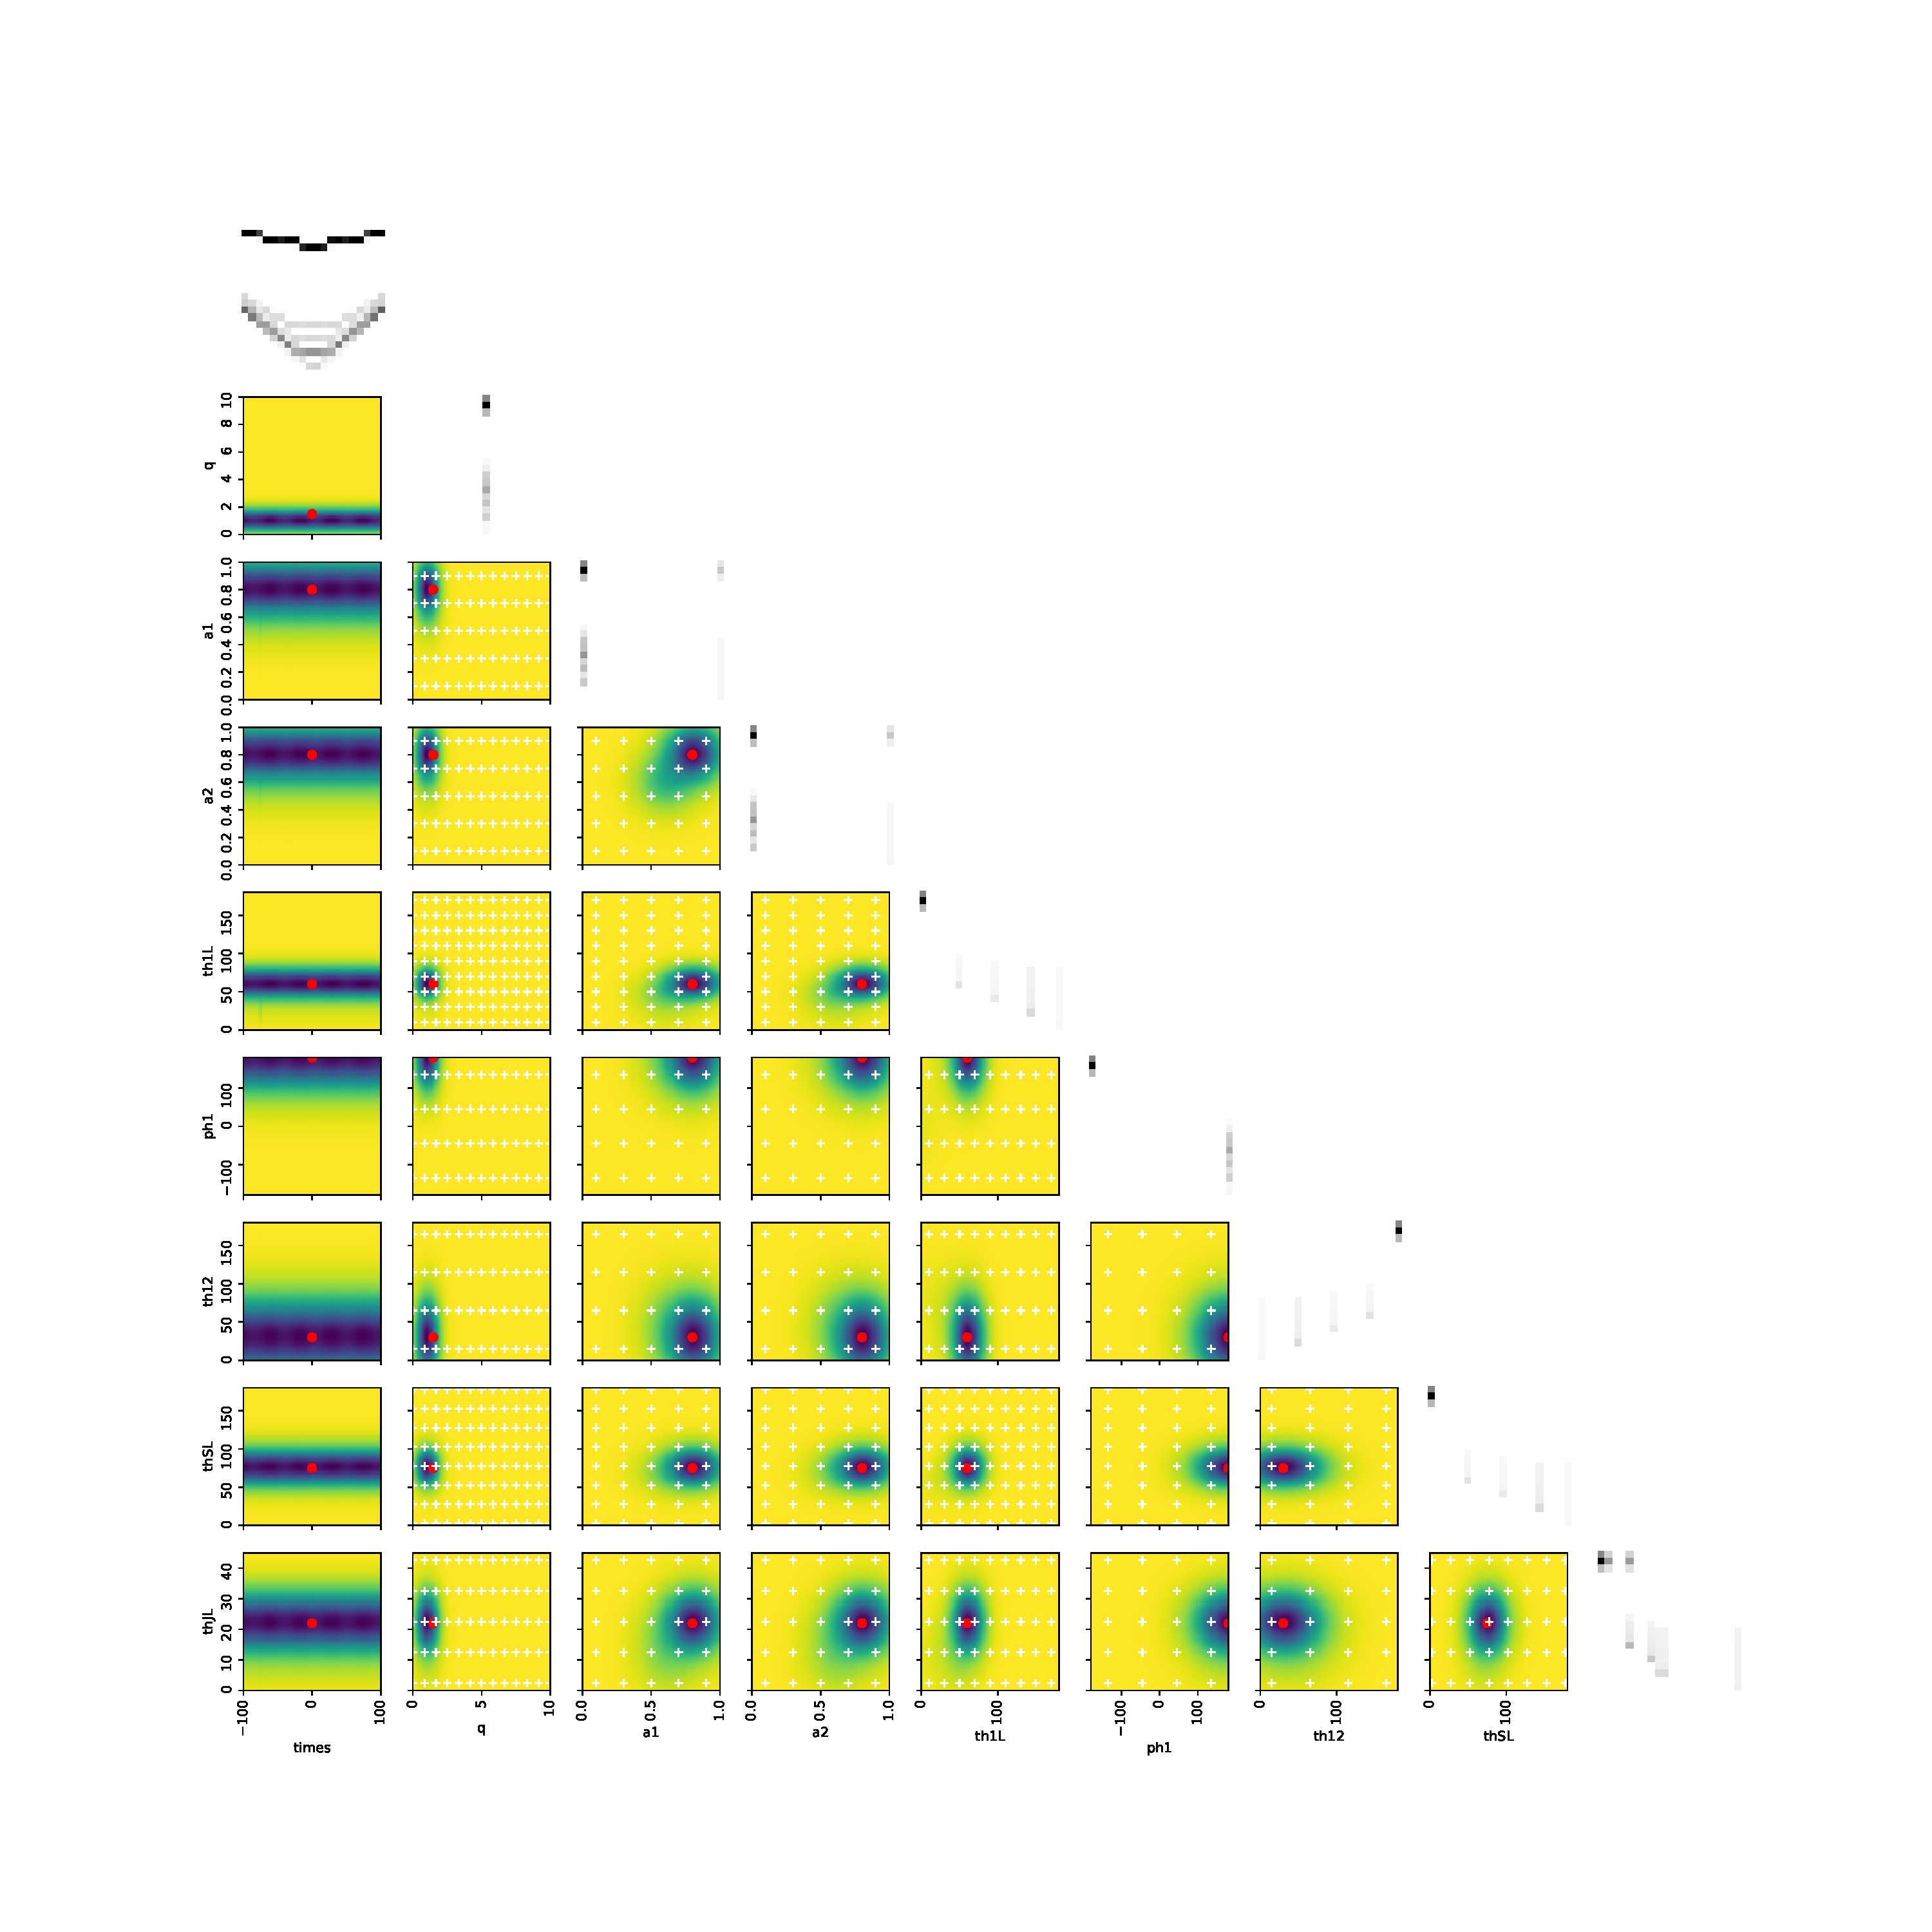
\includegraphics[scale=0.35]{figures/spacings.pdf}
    \caption{A corner plot of a `hyperslice' the parameter space of the numerical relativity waveforms centred on $(t=0,  q=1.5,    a_1=0.8,    a_2=0.8,   \theta_{1L}=60. ,  \phi_1 = 180. ,   \theta_{12} = 30. ,   \theta_{SL} = 75. ,   \theta_{JL} = 22. )$, showing the variation in the magnitude of the Gaussian process uncertainty over the parameter space in the colorplot, and the optimal spacing as implied by the width of the covariance function. The plots above each column are designed to provide a guide to the density of samples throughout the parameter space in that dimension, while the red point represents the point of intersection of the various planes. The Gaussian process used to produce these uncertainty estimates was trained off entire waveforms, including time domain information, but represents a series of slices which intersect at $(t=0,  q=1.5,    a_1=0.8,    a_2=0.8,   \theta_{1L}=60. ,  \phi_1 = 180. ,   \theta_{12} = 30. ,   \theta_{SL} = 75. ,   \theta_{JL} = 22. )$}
  \label{fig:optimal-spacings}
\end{figure}

The magnitude of the Gaussian process error provides a means of
detecting regions of the parameter-space which are poorly understood,
and regions of high uncertainty should then be targeted for future
simulations in order to improve the validity of the surrogate function
across the entire parameter space. The values of $\lambda_{ab}$ define
a metric on the parameter space, and thus a suggested spacing for
these new waveforms, which should be sampled at intervals of
$\log(\lambda_{ab})$, for $\lambda_{ab} \in \Lambda$, in regions with
high uncertainty or regions outwith the parameter-space region defined
by the original training data. Figure \ref{fig:optimal-spacings} shows an
9-dimensional slice in the parameter space of the BBH waveforms from a
Gaussian process trained off ten waveforms. We can see that even with
a small number of waveforms it is possible to provide some estimate of
the correct grid sampling scale-length required to complete the
model\footnote{For simplicity a hypercube lattice is illustrated in
  figure \ref{fig:optimal-spacings}, however, more efficient lattice patterns
  exist to which the scale-length can be applied.}.

In order to demonstrate that the parameter spacing is reasonably
independent of the number of waveforms used in training the GP the
model was generated with a differing number of training waveforms, and
trained. The scale length for each parameter is found to be
consistently similar, as can be seen in figure \ref{fig:convergence}.

\begin{figure}
  \centering
  \includegraphics[width=\textwidth]{figures/convergence.pdf}
  \caption{The difference in the scale-lengths of the trained Gaussian process given 10, 29, 72, 164, and 324 waveforms, compared to the GP trained from 10 waveforms.}
  \label{fig:convergence}
\end{figure}

Having established the optimal spacing of future waveforms we must
then turn to the question of the optimal order in which they should be
created. Sampling the entire parameter space at the suggested density
would require in excess of 250,000 waveforms, which is an unachievably
large quantity of data.

In other fields which exploit Gaussian processes the choice of future
sample locations can be made using techniques from Bayesian
optimisation. In these fields the Gaussian process is often emulating
the behaviour of a complicated function surface, and the desired
outcome is finding an optimum on this surface, for example, if a GP is
used to model the distribution of pollutants in a lake, with the aim
of identifying the source of the pollution we may want to find the
region with the maximum amount of pollutant. 

In the case of gravitational waveform modelling we are not terribly
interested in the location of the function's maximum, but instead have
the objective of achieving the greatest quantity of knowledge possible
in the shortest possible period of time (or equivalently, with the
smallest number of function evaluations). In this case the choice of
future samples might be made to minimise the mean-squared error of the
model.

Using methods based-on the use of testing data requires some of the
available training data to be set-aside, and not used to train the
Gaussian process. Given the small number of samples available, and the
large volume of the parameter space this is likely to have a
considerable impact on the predictive capability of the model. Other
options are available, such as comparing the output to an analytical
model, for example \texttt{IMRPhenomP}, but these approaches suffer
from the incomplete understanding of the uncertainties in these
models.

One possible approach is to simply use the metric defined on the
parameter space by the Gaussian process to determine the location
which is geometrically furthest from any pre-existing training point
in the parameter space. A search of this type can be done efficiently
using voronoi tesselations to rapidly indentify points in the
parameter space which are most distant from any other point. This
approach is clearly \emph{exploration}-driven, where the parameter
space is sampled as widely as possible to get an overview of the
entire underlying function.

An alternative approach is to again use the grid spacing to identify
the closest location to the pre-existing samples which has an
uncertainty greater than some pre-defined threshold in the Gaussian
process model. This approach would fill-in ``holes'' in the parameter
space, working outwards from the existing samples.

A third approach is to allow this planning stage to be informed by the
population distribution of observed signals, and to attempt to improve
the model in order to produce the highest quality waveforms in the
regions of parameter space which are known to represent actualy BBH
systems, that is, which have parameters comparable to those seen in
previous observations.



In the last year I've developed additionally developed a working
protoype of multiple-input, multiple-output Gaussian process
regression in Python, although due to the considerable computational
resources required I have yet to apply this to real-world
data. However, this approach should allow the production of a Gaussian
process surrogate model which is capable of producing both
polarisations of the gravitational waveform for a BBH event. A number
of computational improvements could be made, including parallelising
the training process, which may make this possible.

I am currently in the process of writing-up the initial stages of this
work (the method of using a trained Gaussian process surrogate for
waveform placement) into a paper.

\section{Minke: Producing MDCs for gravitational wave transient analysis}
\label{sec:mink-prod-mdcs}

In order to characterise the efficiency of any gravitational wave
analysis algorithm it must be tested on injected signals---simulated
signals with known parameters, and hence a known shape---which are
inserted into either simulated noise, or timeseries containing real
noise from the detector. By determining the number of these injected
signals which are detected by an algorithm it is possible to determine
the detection efficiency of the method; additionally, this method
allows a controlled method of determining the quietest events the
algorithm is capable of detecting in the noise environment, and hence
of calculating the sensitive distance of the detector and analysis to
a physical system producing a waveform with those parameters. These
tests are known as ``Mock Data Challenges'' (MDCs).

So that consistent results can be produced between the various
different search pipelines it is necessary to generate these
injections via an independent method; previous methods for doing this
within the LSC's burst group have been difficult to maintain or
ad-hoc; ``Minke'' is an attempt to produce an extensible and pythonic
framework for producing burst signal sets, either for use in MDCs, or
for other purposes, such as training machine learning classifiers.

The majority of the initial development on Minke was carried out in
the first six months of my PhD, however I have continued its
development over the last year, with major early achievements being
the implementation and testing of supernova numerical relativity
waveform support, where supernova waveforms which are pre-calculated
by numerical relativity simulations can be injected into detector
data, and the review of the code prior to the pulication of the O1
Burst Search paper\cite{2017PhRvD..95d2003A}, which made use of MDC
sets produced by Minke. Verion 1.0 of ``Minke'' was released on 14
September 2016\footnote{``Minke'' is open source, and both the
  source-code and releases are available on Github at
  \www{http://www.github.com/transientunatic/minke}.}.
During the same period I have been a co-author on a short-author list
paper, and the lead author on a paper composing the write-up of my
MSci project.

I had initially planned development to continue in the direction of
adding support for numerical relativity BBH waveforms to the package,
however this proved difficult due to the lack of a firm standard for
the storage of these waveforms (this standard was finally agreed upon
in March 2017 \cite{2017arXiv170301076S}, and so adding support for
these waveforms has become a short-term goal in the future. Instead I
have focussed further development on adding support for numerical
models such as accretion disk instabilities to the package, and the
ability to generate data which can be used to generate hardware
injections in the detectors. At the time of writing neither of these
new features had been fully reviewed, however review of at least the
hardware injection feature is likely to be required prior to the
publication of a future joint O1/O2 supernova search paper.


\section{Estimating beaming angles from sGRBs}
\label{sec:estim-beam-angl}

\sidebar{

  \begin{tikzpicture}
      % Y
  \node[latent]  (theta)   {$\theta$}; %

  % input distributions
  \node[obs, above = 1.2 of theta] (Rbns)   {$R_{\mathrm{bns}}$}; %
  
  \node[latent, left = of Rbns]  (eff)   {$\epsilon$}; %
  \node[obs, right = of Rbns] (Rgrb) {$R_{\mathrm{grb}}$};
  % eff hyperparameters
  \node[const, above=1.2 of eff, xshift=-0.5cm] (mw) {$h_1$} ; %
  \node[const, above=1.2 of eff, xshift=0.5cm]  (aw) {$h_2$} ; %
  % Rbns hyperparameters
  %\node[const, above=1.2 of Rbns, xshift=-0.5cm] (mx) {$\mu_x$} ; %
  %\node[const, above=1.2 of Rbns, xshift=0.5cm]  (ax) {$\alpha_x$} ; %
   % Factors
  \factor[above=of eff] {eff-f} {left:$\mathcal{D}$} {mw,aw} {eff} ; %
  \edge[-] {eff, Rbns} {theta};
  \edge[-] {Rgrb} {theta};
\end{tikzpicture}
\captionof{figure}{A graphical representation of the hierarchical model used to infer the beaming angle of soft gamma ray bursts from the observed binary neutron star coalesence rate. \label{fig:grb-graph-model}}
}
I have been working in collaboration with James Clark at Georgia
Institute of Technology on developing a method for estimating the
lower-limit on the beaming angle of soft gamma ray bursts (sGRBs)
which result from binary neutron star (BNS) mergers.

This is made possible thanks to knowledge of the posterior probability
distribution on the rate of BNS mergers, which can be determined from
the number of such events which are observed by Advanced LIGO
(although, at the time of writing, this number was zero), and
knowledge of the rate of observed soft gamma ray bursts. A
hierarchical Bayesian analysis can then be used to infer the
probability distribution on the ``opening angle'' of the sGRB.

We can model the observed distribution of gamma ray bursts given
knowledge of the rate of binary neutron star (BNS) mergers as
\begin{equation}
  \label{eq:grb-rate}
  \mathcal{R}_{\mathrm{grb}} = \epsilon \mathcal{R}_{\mathrm{bns}} \left\langle 1 - \cos\theta \right\rangle,
\end{equation}
with $\mathcal{R}_{\mathrm{grb}}$ the observed rate of gamma ray
bursts, $\mathcal{R}_{\mathrm{bns}}$ the observed rate of binary
neutron star coalescences, $\epsilon$ the efficiency at which a BNS
produces a GRB, and $\theta$ the beaming angle. Since two of these
quantities are observable, we can infer $\theta$ by placing a prior on
$\epsilon$, producing a model as depicted in figure
\ref{fig:grb-graph-model}, where $\mathcal{D}(h_1, h_2)$ represents
some prior distribution with two hyperparameters.

\begin{figure}
  \centering
  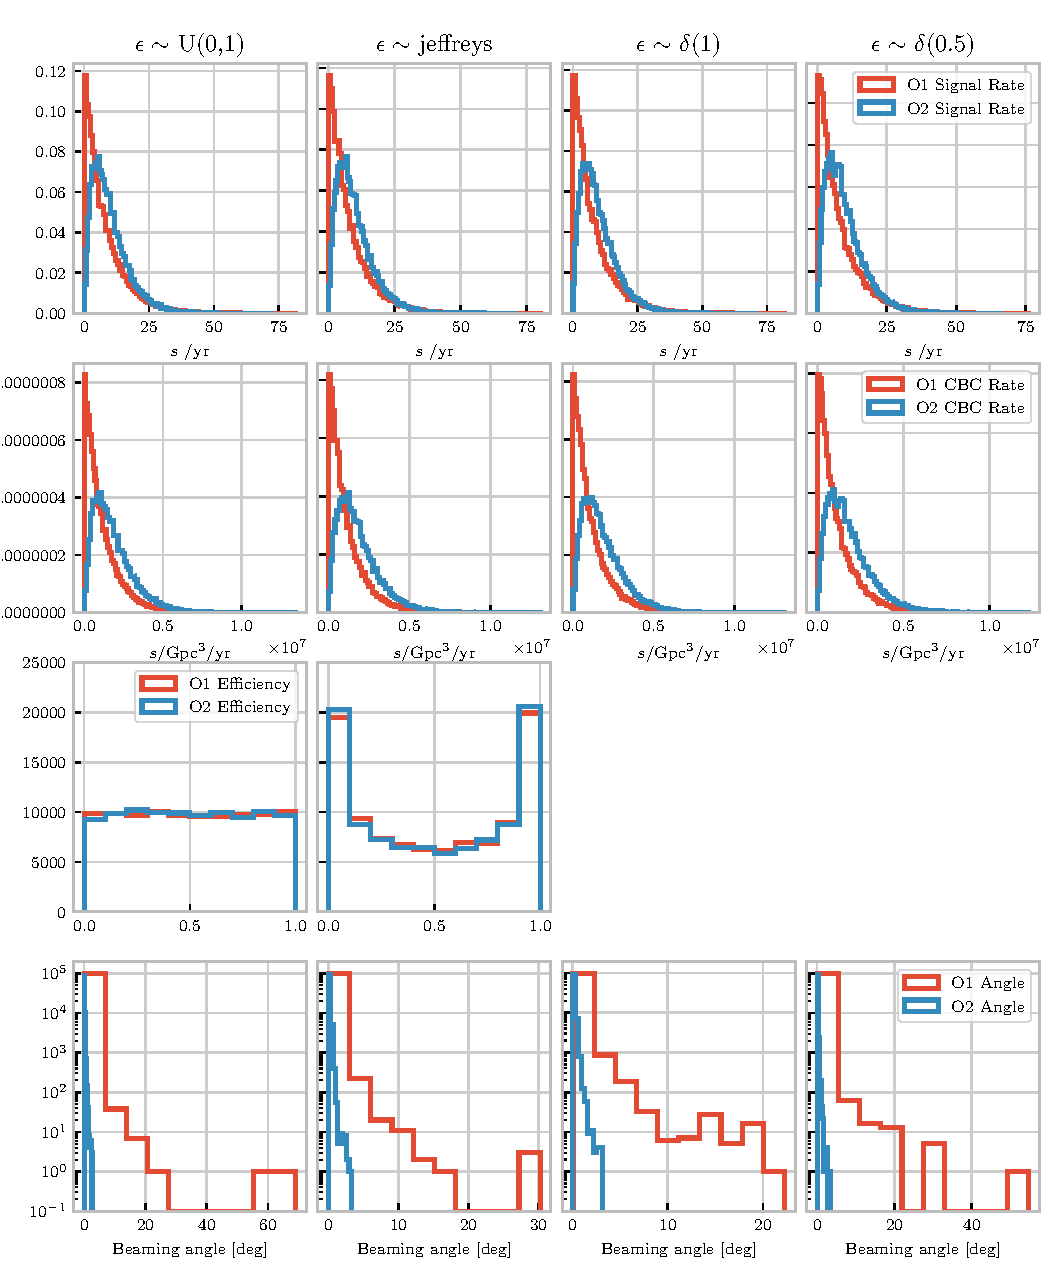
\includegraphics{figures/grbbeamingpymc.pdf}
  \caption{Distributions in the modelling of the GRB beaming angle
    given two observing scenarios; the first aLIGO observing run (O1)
    in which no BNS events were seen, and a speculative, longer second
    observing run (O2) in which one event is seen. Each column
    represents evaluation of the model with a different prior, which
    is specified at the top of the column. Between the top two rows an
    additional conversion is made between the observed signal rate and
    the actual BNS rate.}
  \label{fig:grb-distributions}
\end{figure}

The distribution on $\theta$ can then be inferred using an MCMC
process to sample the posterior. Results for an evaluation of such a
model are shown in figure \ref{fig:grb-distributions}.


%
% A little more detail here would not go amiss
% 

\section{Filter Modeling for glitch tracing in Advanced LIGO}
\label{sec:glitchtracing}

During the course of my long-term attachment at the LIGO site at
Livingston, Louisiana I have been working on developing a system for
modelling the digital signal processing system employed during data
acquisition and detector control at the site. When one of the filters
in this system becomes unstable it can produce a ``glitch'', a
transient noise event in the data from a sensor, or, in the worst
cases, in the DARM read-out channel, which is used to calculate the
gravitational wave strain observed by the detector.

The majority of the digital signal processing system is designed using
Simulink, and the entire system consists a few hundred models which
work in parallel, and which combine multiple input signals. As a
result, tracing the source of a signal which produces a glitch is
non-trivial, and the structure of the signal processing chain acts to
obfuscate the origin of glitch-producing faults.

The signal processing system can be modelled as a directed graph,
allowing graph theoretic algorithms to be used to traverse the system,
and trace the processing of a signal across numerous Simulink models
in order to identify the cause of filter instabilities. My work at
LIGO thus far has mostly revolved around development of a Python
codebase which is capable of parsing Simulink models and filter
definition files in order to run such an analysis.


\appendices

\chapter{Outline of future work}
\label{part:future}
%\chapterprecis{}
\input{tex/5-future}
\backmatter

\newgeometry{left=3cm}

\bibliographystyle{unsrt}
\bibliography{bibliography/introduction,bibliography/relativity,bibliography/detectors,bibliography/gw150914,bibliography/sources,bibliography/analysis,bibliography/gaussian}

% The glossary
\newglossaryentry{gravitational wave}{
  name = {gravitational wave},
  description = {A gravitational wave is a propogating perturbation of spacetime.}
}

\newglossaryentry{GW150914}{
  name = {GW150914},
  description = {The first gravitational wave event to be observed. The observation was made by the two \gls{LIGO} detectors in the United States of America, located at Hanford, Washington; and Livingston, Louisiana}
}

\newglossaryentry{VIRGO}{
  name = {VIRGO},
  description = {
    A gravitational wave detector in Italy.
  }
}

\newglossaryentry{LIGO}{
  name = LIGO,
  description = {
    The Laser Interferometer Gravitational-wave Observatory is a
    joint project of California Institute of Technology (CalTech) and
    the Massechusets Institute of Technology (MIT), in which laser
    interferometers of a similar design to the Michelson
    interferometer, famous for its use in disproving the existence of
    the ``luminous aether'', are used to detect small length
    perturbations over distances of 4km. }
}

\newglossaryentry{DetChar}{
  name = detector characterisation,
  description = {DetChar, or detector characterisation, is the process of analysing the noise sources and calibration of the detector, as well as identifying ``glitches'', transient noise events which can interfere with burst searches, and ``lines'', sources of noise which exist in a narrow frequency band which can interfere with long-integration time searches.}
}

\newglossaryentry{burst}{
  name = burst,
  description = {A burst is a short-lived, transient gravitational wave event.}
}

\newglossaryentry{chirp mass}{
  name = {chirp mass, $\mathcal{M}$},
  description = {
    The chirp mass of a binary system is defined as 
    \[ \mathcal{M} = \frac{ (m_1 m_2)^{3/5} }{(m_1 + m_2)^{1/5} } \]
    for $m_1$ and $m_2$ the masses of the two components of the binary,
    and determines the amplitude and the frequency evolution of a
    chirp from a coalescence%
  }}

\newglossaryentry{SNR}{
  name = {signal-to-noise ratio, SNR},
  description = {
    The ratio of signal power to noise power in a given signal. For a
    gravitational wave detector it is defined
    \[ \rho^2 = \int_0^\infty \frac{ 4 \left| h(f) \right|^2
    }{S_n(f)} \dd{f} \] for $h(f)$ the strain of the signal in the frequency
    domain, and $S_n$ is the power spectral density of the detector%
  }
}

\newglossaryentry{characteristic strain}{
  name = characteristic strain,
  description = {
    The characteristic strain is designed to take into account the change of a signal's frequency when it is integrated. It is defined
    \[h^2~c(f) = 4 f^2 \abs{h(f)}^2 \] for $h(f)$ the strain of the
    signal in the frequency domain, and $f$ the frequency%
  } }

\newglossaryentry{finesse}{
  name = finesse,
  description = {
The number of times a beam reflects between ends of a Fabry-Perot interferometer.
  } }

%%% Local Variables: 
%%% mode: latex
%%% TeX-master: "../document"
%%% End: 

%\newglossaryentry{cbc}{
  name = {compact binary coalescence},
  description = {
    The collision and merging of two dense, degenerate stellar
    remnants. The typical remnants considered in CBC searches are
    neutrin stars and black holes, although the range of compact
    objects extends to white dwarfs, and possibly exotic remnants,
    such as quark and boson stars
  }
}

\glsaddall
\useglossarystyle{altlist}
\printglossaries

\end{document}
